% Options for packages loaded elsewhere
\PassOptionsToPackage{unicode}{hyperref}
\PassOptionsToPackage{hyphens}{url}
\PassOptionsToPackage{dvipsnames,svgnames,x11names}{xcolor}
%
\documentclass[
  11pt,
  a4paper,
]{book}
\usepackage{amsmath,amssymb}
\usepackage{lmodern}
\usepackage{setspace}
\usepackage{iftex}
\ifPDFTeX
  \usepackage[T1]{fontenc}
  \usepackage[utf8]{inputenc}
  \usepackage{textcomp} % provide euro and other symbols
\else % if luatex or xetex
  \usepackage{unicode-math}
  \defaultfontfeatures{Scale=MatchLowercase}
  \defaultfontfeatures[\rmfamily]{Ligatures=TeX,Scale=1}
  \setmonofont[Scale=0.8]{Consolas}
\fi
% Use upquote if available, for straight quotes in verbatim environments
\IfFileExists{upquote.sty}{\usepackage{upquote}}{}
\IfFileExists{microtype.sty}{% use microtype if available
  \usepackage[]{microtype}
  \UseMicrotypeSet[protrusion]{basicmath} % disable protrusion for tt fonts
}{}
\makeatletter
\@ifundefined{KOMAClassName}{% if non-KOMA class
  \IfFileExists{parskip.sty}{%
    \usepackage{parskip}
  }{% else
    \setlength{\parindent}{0pt}
    \setlength{\parskip}{6pt plus 2pt minus 1pt}}
}{% if KOMA class
  \KOMAoptions{parskip=half}}
\makeatother
\usepackage{xcolor}
\usepackage[lmargin=1in,rmargin=1in,tmargin=1in,bmargin=1in]{geometry}
\usepackage{color}
\usepackage{fancyvrb}
\newcommand{\VerbBar}{|}
\newcommand{\VERB}{\Verb[commandchars=\\\{\}]}
\DefineVerbatimEnvironment{Highlighting}{Verbatim}{commandchars=\\\{\}}
% Add ',fontsize=\small' for more characters per line
\usepackage{framed}
\definecolor{shadecolor}{RGB}{248,248,248}
\newenvironment{Shaded}{\begin{snugshade}}{\end{snugshade}}
\newcommand{\AlertTok}[1]{\textcolor[rgb]{0.94,0.16,0.16}{#1}}
\newcommand{\AnnotationTok}[1]{\textcolor[rgb]{0.56,0.35,0.01}{\textbf{\textit{#1}}}}
\newcommand{\AttributeTok}[1]{\textcolor[rgb]{0.77,0.63,0.00}{#1}}
\newcommand{\BaseNTok}[1]{\textcolor[rgb]{0.00,0.00,0.81}{#1}}
\newcommand{\BuiltInTok}[1]{#1}
\newcommand{\CharTok}[1]{\textcolor[rgb]{0.31,0.60,0.02}{#1}}
\newcommand{\CommentTok}[1]{\textcolor[rgb]{0.56,0.35,0.01}{\textit{#1}}}
\newcommand{\CommentVarTok}[1]{\textcolor[rgb]{0.56,0.35,0.01}{\textbf{\textit{#1}}}}
\newcommand{\ConstantTok}[1]{\textcolor[rgb]{0.00,0.00,0.00}{#1}}
\newcommand{\ControlFlowTok}[1]{\textcolor[rgb]{0.13,0.29,0.53}{\textbf{#1}}}
\newcommand{\DataTypeTok}[1]{\textcolor[rgb]{0.13,0.29,0.53}{#1}}
\newcommand{\DecValTok}[1]{\textcolor[rgb]{0.00,0.00,0.81}{#1}}
\newcommand{\DocumentationTok}[1]{\textcolor[rgb]{0.56,0.35,0.01}{\textbf{\textit{#1}}}}
\newcommand{\ErrorTok}[1]{\textcolor[rgb]{0.64,0.00,0.00}{\textbf{#1}}}
\newcommand{\ExtensionTok}[1]{#1}
\newcommand{\FloatTok}[1]{\textcolor[rgb]{0.00,0.00,0.81}{#1}}
\newcommand{\FunctionTok}[1]{\textcolor[rgb]{0.00,0.00,0.00}{#1}}
\newcommand{\ImportTok}[1]{#1}
\newcommand{\InformationTok}[1]{\textcolor[rgb]{0.56,0.35,0.01}{\textbf{\textit{#1}}}}
\newcommand{\KeywordTok}[1]{\textcolor[rgb]{0.13,0.29,0.53}{\textbf{#1}}}
\newcommand{\NormalTok}[1]{#1}
\newcommand{\OperatorTok}[1]{\textcolor[rgb]{0.81,0.36,0.00}{\textbf{#1}}}
\newcommand{\OtherTok}[1]{\textcolor[rgb]{0.56,0.35,0.01}{#1}}
\newcommand{\PreprocessorTok}[1]{\textcolor[rgb]{0.56,0.35,0.01}{\textit{#1}}}
\newcommand{\RegionMarkerTok}[1]{#1}
\newcommand{\SpecialCharTok}[1]{\textcolor[rgb]{0.00,0.00,0.00}{#1}}
\newcommand{\SpecialStringTok}[1]{\textcolor[rgb]{0.31,0.60,0.02}{#1}}
\newcommand{\StringTok}[1]{\textcolor[rgb]{0.31,0.60,0.02}{#1}}
\newcommand{\VariableTok}[1]{\textcolor[rgb]{0.00,0.00,0.00}{#1}}
\newcommand{\VerbatimStringTok}[1]{\textcolor[rgb]{0.31,0.60,0.02}{#1}}
\newcommand{\WarningTok}[1]{\textcolor[rgb]{0.56,0.35,0.01}{\textbf{\textit{#1}}}}
\usepackage{longtable,booktabs,array}
\usepackage{calc} % for calculating minipage widths
% Correct order of tables after \paragraph or \subparagraph
\usepackage{etoolbox}
\makeatletter
\patchcmd\longtable{\par}{\if@noskipsec\mbox{}\fi\par}{}{}
\makeatother
% Allow footnotes in longtable head/foot
\IfFileExists{footnotehyper.sty}{\usepackage{footnotehyper}}{\usepackage{footnote}}
\makesavenoteenv{longtable}
\usepackage{graphicx}
\makeatletter
\def\maxwidth{\ifdim\Gin@nat@width>\linewidth\linewidth\else\Gin@nat@width\fi}
\def\maxheight{\ifdim\Gin@nat@height>\textheight\textheight\else\Gin@nat@height\fi}
\makeatother
% Scale images if necessary, so that they will not overflow the page
% margins by default, and it is still possible to overwrite the defaults
% using explicit options in \includegraphics[width, height, ...]{}
\setkeys{Gin}{width=\maxwidth,height=\maxheight,keepaspectratio}
% Set default figure placement to htbp
\makeatletter
\def\fps@figure{htbp}
\makeatother
\setlength{\emergencystretch}{3em} % prevent overfull lines
\providecommand{\tightlist}{%
  \setlength{\itemsep}{0pt}\setlength{\parskip}{0pt}}
\setcounter{secnumdepth}{5}
\usepackage{booktabs}
\usepackage{fontspec}
\usepackage{pdfpages}
\usepackage{amsthm}
\makeatletter
\def\thm@space@setup{%
  \thm@preskip=8pt plus 2pt minus 4pt
  \thm@postskip=\thm@preskip
}
\makeatother
\let\oldmaketitle\maketitle
\AtBeginDocument{\let\maketitle\relax}
\ifLuaTeX
  \usepackage{selnolig}  % disable illegal ligatures
\fi
\IfFileExists{bookmark.sty}{\usepackage{bookmark}}{\usepackage{hyperref}}
\IfFileExists{xurl.sty}{\usepackage{xurl}}{} % add URL line breaks if available
\urlstyle{same} % disable monospaced font for URLs
\hypersetup{
  pdftitle={H2 Data Science Practical Series},
  colorlinks=true,
  linkcolor={blue},
  filecolor={Maroon},
  citecolor={Blue},
  urlcolor={blue},
  pdfcreator={LaTeX via pandoc}}

\title{H2 Data Science Practical Series}
\author{}
\date{\vspace{-2.5em}}

\begin{document}
\maketitle

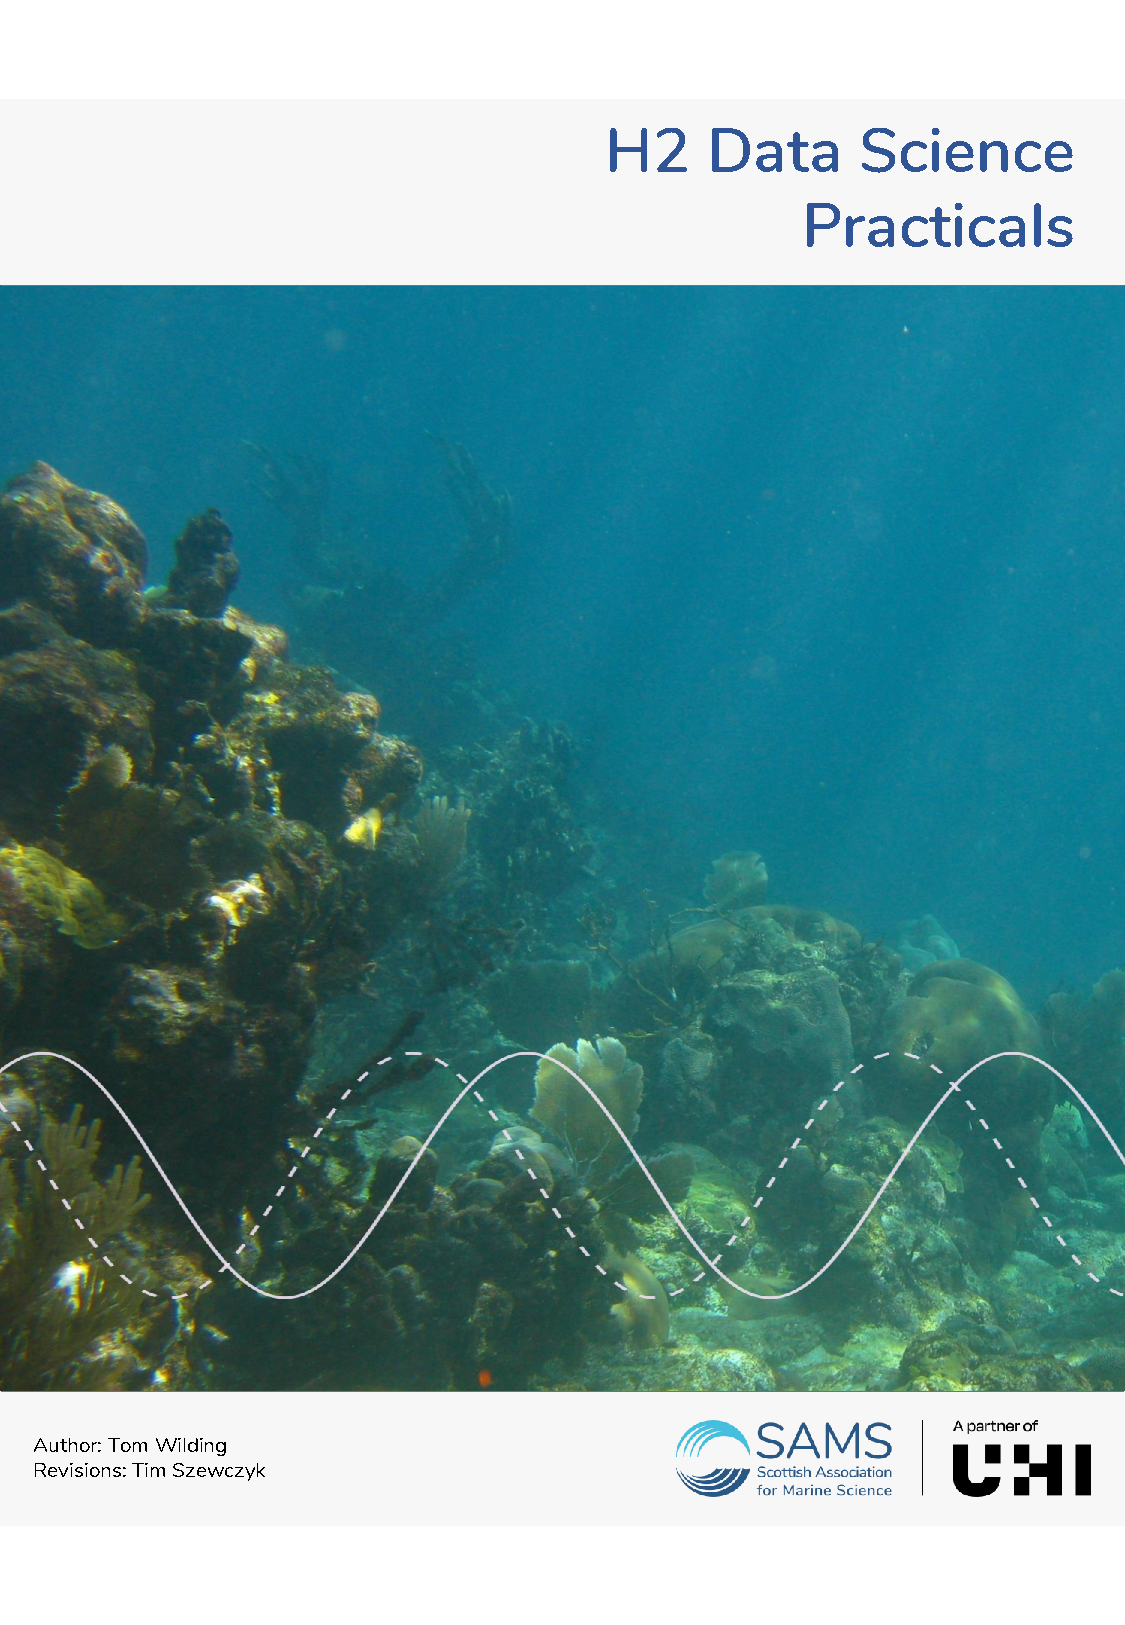
\includepdf[pages={1}, scale=1]{figs/cover.pdf}

\let\maketitle\oldmaketitle


{
\hypersetup{linkcolor=}
\setcounter{tocdepth}{0}
\tableofcontents
}
\setstretch{1}
\hypertarget{overview}{%
\chapter*{Overview}\label{overview}}
\addcontentsline{toc}{chapter}{Overview}

\hypertarget{practical-sessions}{%
\section{Practical sessions}\label{practical-sessions}}

In these practicals, you will practice applying the data science concepts you learn throughout the H2 Data Science course. The questions you answer by hand are useful for learning and revision, while producing appropriate graphics and correctly describing results are essential parts of the scientific process. Expertise in these core skills is essential to do well in future courses and scientific projects. H2 Data Science is, therefore, one of the most important courses you'll take!

In each practical, you will either generate your own data or process and analyse data sets that I have either obtained or generated to illustrate particular points. They are stored in labelled Excel spreadsheets under a variety of named worksheets.

Each session is 2.5h, during which you will work through a series of coding exercises and questions. These are not assessed or marked, but some of them appear in the assessments. You should complete all the material in each practical. My recommendation, particularly for those not comfortable with R, is that you read through the practical before the class.

Throughout the sessions, we will alternate between individual work and short re-caps as a class. If you find yourself racing ahead, all well and good. If you find yourself falling behind, then try some additional study ahead of the next session.

\hypertarget{assessments}{%
\section{Assessments}\label{assessments}}

During this time slot throughout the semester, there will be six practical sessions and three assessments (see the schedule on Brightspace). All three assessments are via Brightspace and consist of multiple choice, single fill-in-the-blank, and slightly more expansive answers. They are `open Brightspace' but timed, so you will need to understand the material and be comfortable working in R to do well in these assessments. You are welcome to bring a hard copy of this booklet with annotations if you wish.

\begin{center}\rule{0.5\linewidth}{0.5pt}\end{center}

\hypertarget{R_intro}{%
\section{Getting started in R}\label{R_intro}}

R is a statistical language and computing platform that is widely used in the sciences. It is free and open source. We will be using it extensively in this course, so I recommend you review your notes and course material from last year to prepare for this course.

There are also fantastic resources available online. In addition to those listed in the module handbook, there are courses such as those from \href{https://swcarpentry.github.io/r-novice-gapminder/}{Software Carpentry} or \href{https://swirlstats.com/}{Swirl}. You should access these resources in your own time to complement, revise, and reinforce the concepts you'll be learning during this course.

Try to avoid copying and pasting code where possible during these practicals. R is best learned through your fingers, and working through errors, though frustrating, is an essential skill.

\hypertarget{rstudio-project}{%
\subsection{RStudio Project}\label{rstudio-project}}

Working in a Project within RStudio is the best way to avoid working directory complications.

Open RStudio, go to `file' then `New project'. Name and save your project (e.g., `H2\_DataScience.Rproj') in a convenient location. OneDrive works, though occasionally gives sync errors with hidden files if you use multiple machines.

Next, in the same folder as your .Rproj, create a folder called \emph{data} and a folder called \emph{code}.

Download the files in \emph{Practicals \textgreater{} data} on Brightspace and move them into your \emph{data} folder.

Your files should be visible under the `Files' tab in R Studio, together with your new project.

The code in the practicals assumes this setup. I recommend creating a separate R script (.R) or R Markdown file (.Rmd) for each practical session, saved within the \emph{code} folder.

Each time you open your .Rproj, the working directory will be set to the enclosing folder. The working directory is shown at the top of the Console pane, and you can check it with \texttt{getwd()}.

\hypertarget{rstudio-settings}{%
\subsection{RStudio Settings}\label{rstudio-settings}}

You can adjust many settings in RStudio via Tools \textgreater{} Global options. In the Appearance tab in the popup box, you can set the theme (e.g., if you prefer a dark theme), font size, etc. The Code tab has many nice features as well (e.g., rainbow parentheses under Display).

\hypertarget{r-packages-and-libraries}{%
\subsection{R packages and libraries}\label{r-packages-and-libraries}}

R packages are collections of functions, custom data structures, and datasets that are developed by the userbase. A new installation of R includes many useful default packages, visible on the `Packages' tab in RStudio. There are many additional packages available from the official CRAN repository or less officially from GitHub. If you find yourself re-using custom functions across projects, you can even create your own personal package.

To install a package from CRAN, use the function \texttt{install.packages("packageName")}. This downloads the package files to your computer. Each time you open R, you will need to load that package to use it with \texttt{library(packageName)}.

Installing from other package sources is slightly more complicated, so see me if you have a need.

You can get an overview of a package with \texttt{?packageName}, and then see a list of all of the functions by scrolling to the bottom of the help page and clicking the ``index'' link.

The help for each function is available with \texttt{?functionName}, and you can see the underlying code with \texttt{functionName} without parentheses.

\hypertarget{EDA}{%
\chapter{Displaying and summarising data}\label{EDA}}

Statistics can be divided into two broad categories - descriptive statistics and inferential statistics. In this practical session we will focus on descriptive stats and, in particular, how to appropriately display and summarise data. You should already be aware of several techniques for displaying data. These techniques are primarily graphical and include bar charts, histograms and graphs. When and how to use these different techniques is one focus of today's practical.

There are two purposes for visualizing data.

First, the best way to get a `gut' feel for your dataset is to look at it graphically. Examining data graphically enables you to identify any outliers (i.e., suspicious observations which could be errors). It will also help you to select the most appropriate inferential statistical model (more on this through the course).

Second, visualizations are used to impart information as clearly as possible to `the reader' (i.e., drawing the reader's attention to the most interesting aspects of your data). Graphics that are confusing, either through a lack of detail (e.g.~no labels) or that contain too much information will fail in this central objective.

As you create graphics, keep in mind that they may be viewed on different machines or printed in grey scale. Importantly, some colour combinations may be difficult for colour-blind or visually impaired readers. Colour scales such as those available from \href{https://colorbrewer2.org}{ColorBrewer} or \href{https://cran.r-project.org/web/packages/viridis/vignettes/intro-to-viridis.html}{viridis} are designed with this in mind.

R has established best practices to make your meaning clear. Just like any language, you\textbar can\textbar write\textbar with\textbar your\textbar own\textbar system, but it's easier for everyone to use standard conventions. A \href{https://style.tidyverse.org/syntax.html}{full style guide} is available if you're interested.

A few key points:

\begin{itemize}
\tightlist
\item
  Use \texttt{\textless{}-} to \emph{assign} a value to an object. You may see \texttt{=}, which works, but is not preferred.
\item
  Use spaces to make your code legible: \texttt{a\ \textless{}-\ 10}; \texttt{mean(x,\ na.rm=T)}; \texttt{c(1,\ 2,\ 3)}.
\item
  Avoid spaces in column or file names (in general) as these are a pain to work with.
\item
  Use names for objects that are short, but descriptive.
\item
  Limit the length of a line of code to about 80 characters.
\item
  Usually, variables should be nouns and functions should be verbs.
\item
  Use \texttt{\#} to write a comment which R will ignore.
\item
  Run the line of code where your cursor is (or everything you've selected) with ctrl+r
\end{itemize}

\begin{center}\rule{0.5\linewidth}{0.5pt}\end{center}

\hypertarget{basic-data-exploration}{%
\section{Basic data exploration}\label{basic-data-exploration}}

We will mostly be working with dataframes. A dataframe is a 2D rectangular structure with columns and rows. In a tidy dataset, each row represents an `observation' and each column represents a `variable'. R (and often packages) contains several built-in dataframes.

The dataframe \texttt{cars} gives the max speeds and stopping distances for cars built in the early 20th century. We are going to use this dataset as a starting point to demonstrate a few basic concepts in relation to R programming and statistical analysis.

\begin{Shaded}
\begin{Highlighting}[]
\CommentTok{\# functions for basic details of objects}
\FunctionTok{str}\NormalTok{(cars)}
\FunctionTok{class}\NormalTok{(cars)}
\FunctionTok{names}\NormalTok{(cars)}
\FunctionTok{head}\NormalTok{(cars)}
\end{Highlighting}
\end{Shaded}

\begin{Shaded}
\begin{Highlighting}[]
\FunctionTok{head}\NormalTok{(cars, }\DecValTok{2}\NormalTok{)}
\end{Highlighting}
\end{Shaded}

\begin{verbatim}
##   speed dist
## 1     4    2
## 2     4   10
\end{verbatim}

\begin{Shaded}
\begin{Highlighting}[]
\FunctionTok{tail}\NormalTok{(cars, }\DecValTok{2}\NormalTok{)}
\end{Highlighting}
\end{Shaded}

\begin{verbatim}
##    speed dist
## 49    24  120
## 50    25   85
\end{verbatim}

\begin{Shaded}
\begin{Highlighting}[]
\CommentTok{\# what are the last 10 rows?}
\end{Highlighting}
\end{Shaded}

There are several ways to access subsets of a dataframe:

\begin{itemize}
\tightlist
\item
  Use \texttt{.\$columnName} or \texttt{.{[}{[}"columnName"{]}{]}} to extract a single column
\item
  Use \texttt{.{[}rows,columns{]}} to extract a block
\end{itemize}

\begin{Shaded}
\begin{Highlighting}[]
\NormalTok{cars}\SpecialCharTok{$}\NormalTok{speed}
\NormalTok{cars[[}\StringTok{"speed"}\NormalTok{]]}
\end{Highlighting}
\end{Shaded}

\begin{Shaded}
\begin{Highlighting}[]
\NormalTok{cars[}\DecValTok{1}\NormalTok{, }\DecValTok{1}\NormalTok{] }\CommentTok{\# row 1, column 1}
\end{Highlighting}
\end{Shaded}

\begin{verbatim}
## [1] 4
\end{verbatim}

\begin{Shaded}
\begin{Highlighting}[]
\NormalTok{cars[}\DecValTok{1}\SpecialCharTok{:}\DecValTok{5}\NormalTok{, }\DecValTok{1}\NormalTok{]}
\end{Highlighting}
\end{Shaded}

\begin{verbatim}
## [1] 4 4 7 7 8
\end{verbatim}

\begin{Shaded}
\begin{Highlighting}[]
\NormalTok{cars[}\DecValTok{1}\SpecialCharTok{:}\DecValTok{3}\NormalTok{, ] }\CommentTok{\# leaving the columns blank returns all columns}
\end{Highlighting}
\end{Shaded}

\begin{verbatim}
##   speed dist
## 1     4    2
## 2     4   10
## 3     7    4
\end{verbatim}

We can also change column names. We'll make a copy of the dataframe to do that.

Rearranging and duplicating columns is also easy.

\begin{Shaded}
\begin{Highlighting}[]
\FunctionTok{head}\NormalTok{(cars2, }\DecValTok{2}\NormalTok{) }
\end{Highlighting}
\end{Shaded}

\begin{verbatim}
##   speed_mph dist_ft
## 1         4       2
## 2         4      10
\end{verbatim}

\begin{Shaded}
\begin{Highlighting}[]
\NormalTok{cars2}\SpecialCharTok{$}\NormalTok{speed\_mph }
\end{Highlighting}
\end{Shaded}

\begin{verbatim}
##  [1]  4  4  7  7  8  9 10 10 10 11 11 12 12 12 12 13 13 13 13 14 14 14 14 15 15
## [26] 15 16 16 17 17 17 18 18 18 18 19 19 19 20 20 20 20 20 22 23 24 24 24 24 25
\end{verbatim}

\begin{Shaded}
\begin{Highlighting}[]
\NormalTok{cars2 }\OtherTok{\textless{}{-}}\NormalTok{ cars2[, }\DecValTok{2}\SpecialCharTok{:}\DecValTok{1}\NormalTok{] }
\FunctionTok{head}\NormalTok{(cars2, }\DecValTok{2}\NormalTok{) }
\end{Highlighting}
\end{Shaded}

\begin{verbatim}
##   dist_ft speed_mph
## 1       2         4
## 2      10         4
\end{verbatim}

\begin{Shaded}
\begin{Highlighting}[]
\NormalTok{cars3 }\OtherTok{\textless{}{-}}\NormalTok{ cars2[, }\FunctionTok{c}\NormalTok{(}\DecValTok{2}\NormalTok{, }\DecValTok{1}\NormalTok{, }\DecValTok{1}\NormalTok{)] }\CommentTok{\# duplicate a column}
\FunctionTok{head}\NormalTok{(cars3, }\DecValTok{2}\NormalTok{)}
\end{Highlighting}
\end{Shaded}

\begin{verbatim}
##   speed_mph dist_ft dist_ft.1
## 1         4       2         2
## 2         4      10        10
\end{verbatim}

\begin{Shaded}
\begin{Highlighting}[]
\NormalTok{cars3 }\OtherTok{\textless{}{-}}\NormalTok{ cars3[, }\FunctionTok{c}\NormalTok{(}\DecValTok{2}\NormalTok{, }\DecValTok{1}\NormalTok{)] }\CommentTok{\# remove the duplicated column}
\FunctionTok{head}\NormalTok{(cars3, }\DecValTok{2}\NormalTok{)}
\end{Highlighting}
\end{Shaded}

\begin{verbatim}
##   dist_ft speed_mph
## 1       2         4
## 2      10         4
\end{verbatim}

\begin{Shaded}
\begin{Highlighting}[]
\NormalTok{cars3}\SpecialCharTok{$}\NormalTok{dist\_x\_speed }\OtherTok{\textless{}{-}}\NormalTok{ cars3}\SpecialCharTok{$}\NormalTok{dist\_ft }\SpecialCharTok{*}\NormalTok{ cars3}\SpecialCharTok{$}\NormalTok{speed\_mph }\CommentTok{\# create a new column}
\FunctionTok{head}\NormalTok{(cars3, }\DecValTok{2}\NormalTok{)}
\end{Highlighting}
\end{Shaded}

\begin{verbatim}
##   dist_ft speed_mph dist_x_speed
## 1       2         4            8
## 2      10         4           40
\end{verbatim}

\begin{Shaded}
\begin{Highlighting}[]
\FunctionTok{rm}\NormalTok{(cars3) }\CommentTok{\# remove the dataframe \textquotesingle{}cars3\textquotesingle{}}
\end{Highlighting}
\end{Shaded}

You can also subset based on criteria. Say we only want rows where the speed is \(>\) 20 mph:

\begin{Shaded}
\begin{Highlighting}[]
\NormalTok{a }\OtherTok{\textless{}{-}} \FunctionTok{which}\NormalTok{(cars2}\SpecialCharTok{$}\NormalTok{speed\_mph }\SpecialCharTok{\textgreater{}} \DecValTok{20}\NormalTok{) }
\FunctionTok{str}\NormalTok{(a)}
\end{Highlighting}
\end{Shaded}

\begin{verbatim}
##  int [1:7] 44 45 46 47 48 49 50
\end{verbatim}

\begin{Shaded}
\begin{Highlighting}[]
\NormalTok{cars\_fast }\OtherTok{\textless{}{-}}\NormalTok{ cars2[a, ] }\CommentTok{\# or: cars2[which(cars2$speed\_mph \textgreater{} 20), ]}
\FunctionTok{class}\NormalTok{(cars\_fast) }
\end{Highlighting}
\end{Shaded}

\begin{verbatim}
## [1] "data.frame"
\end{verbatim}

\begin{Shaded}
\begin{Highlighting}[]
\FunctionTok{ncol}\NormalTok{(cars\_fast)  }\CommentTok{\# and how many *rows* are there?}
\end{Highlighting}
\end{Shaded}

\begin{verbatim}
## [1] 2
\end{verbatim}

\begin{Shaded}
\begin{Highlighting}[]
\FunctionTok{head}\NormalTok{(cars\_fast, }\DecValTok{2}\NormalTok{)}
\end{Highlighting}
\end{Shaded}

\begin{verbatim}
##    dist_ft speed_mph
## 44      66        22
## 45      54        23
\end{verbatim}

When you import data, you should check for missing values. These are represented as \texttt{NA}.

We can check each element of a vector using \texttt{is.na()}, which will return \texttt{FALSE} if an element \emph{is not} \texttt{NA}, and \texttt{TRUE} if an element \emph{is} \texttt{NA}.

\begin{Shaded}
\begin{Highlighting}[]
\FunctionTok{is.na}\NormalTok{(cars2}\SpecialCharTok{$}\NormalTok{speed\_mph)}
\end{Highlighting}
\end{Shaded}

R converts a logical vector (i.e., \texttt{TRUE}/\texttt{FALSE}) to numeric (i.e., \texttt{1}/\texttt{0}) automatically. This is handy, but dangerous if you don't realize it.

\begin{Shaded}
\begin{Highlighting}[]
\FunctionTok{sum}\NormalTok{(}\FunctionTok{is.na}\NormalTok{(cars2}\SpecialCharTok{$}\NormalTok{speed\_mph))}
\end{Highlighting}
\end{Shaded}

\begin{verbatim}
## [1] 0
\end{verbatim}

\begin{Shaded}
\begin{Highlighting}[]
\NormalTok{carsNA }\OtherTok{\textless{}{-}}\NormalTok{ cars2}
\NormalTok{carsNA[}\FunctionTok{c}\NormalTok{(}\DecValTok{2}\NormalTok{, }\DecValTok{4}\NormalTok{, }\DecValTok{5}\NormalTok{, }\DecValTok{10}\NormalTok{), }\DecValTok{1}\NormalTok{] }\OtherTok{\textless{}{-}} \ConstantTok{NA}
\FunctionTok{sum}\NormalTok{(}\FunctionTok{is.na}\NormalTok{(carsNA}\SpecialCharTok{$}\NormalTok{dist\_ft))}
\end{Highlighting}
\end{Shaded}

\begin{verbatim}
## [1] 4
\end{verbatim}

Another very useful check is \texttt{summary()}:

\begin{Shaded}
\begin{Highlighting}[]
\FunctionTok{summary}\NormalTok{(cars)}
\end{Highlighting}
\end{Shaded}

\begin{verbatim}
##      speed           dist       
##  Min.   : 4.0   Min.   :  2.00  
##  1st Qu.:12.0   1st Qu.: 26.00  
##  Median :15.0   Median : 36.00  
##  Mean   :15.4   Mean   : 42.98  
##  3rd Qu.:19.0   3rd Qu.: 56.00  
##  Max.   :25.0   Max.   :120.00
\end{verbatim}

\begin{Shaded}
\begin{Highlighting}[]
\FunctionTok{summary}\NormalTok{(carsNA)}
\end{Highlighting}
\end{Shaded}

Once you have assured yourself that your dataframe looks sensible, that it contains the data you expect, and that you know what the data-types are, you can start to explore and summarise your data.

There are many graphical methods for data exploration and it is important to select the appropriate method. This will be determined by the nature of the data and what you wish to communicate to the reader.

\begin{center}\rule{0.5\linewidth}{0.5pt}\end{center}

\hypertarget{graphical-methods-for-displaying-data}{%
\section{Graphical methods for displaying data}\label{graphical-methods-for-displaying-data}}

Always keep in mind that the primary reason for data visualization is to impart information concisely and accurately to your reader.

Graphics must be clear, concise and easy to understand. Brightspace contains some examples of bad graphics (`Learning resources\textgreater Lecture support material\textgreater Introduction (Lectures 1-3)\textgreater Graphics').

\begin{figure}
\centerline{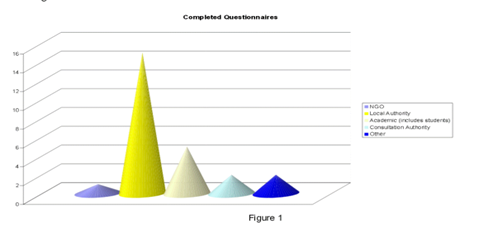
\includegraphics[width=0.5\textwidth]{figs/bad_fig_1.png}}
\caption{An example of a terrible graphic, as published in a Scottish government report.}
\label{fig:bad1}
\end{figure}

In addition to poor design choices for effective communication (Fig. \ref{fig:bad1}), graphics can also be deliberately misleading (Fig. \ref{fig:bad2}).

\begin{figure}
\centerline{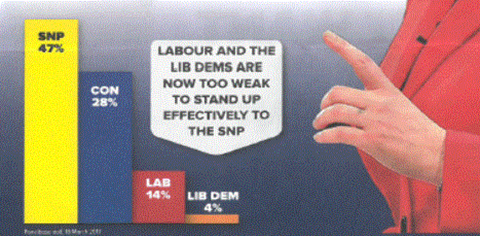
\includegraphics[width=0.5\textwidth]{figs/bad_fig_2.png}}
\caption{A misleading graphic. What type of plot is this and how is it misleading?}
\label{fig:bad2}
\end{figure}

\hypertarget{scatter-plot}{%
\subsection{Scatter plot}\label{scatter-plot}}

The scatter plot is used where you are plotting two continuous variables against each other. It can be used to check whether outliers are present in your data. This is the plot to use if you are doing a correlation analysis and you need to show the raw data to your reader.

\begin{Shaded}
\begin{Highlighting}[]
\CommentTok{\# plot(reponse \textasciitilde{} predictor, data = dataframe)}
\FunctionTok{plot}\NormalTok{(dist\_ft }\SpecialCharTok{\textasciitilde{}}\NormalTok{ speed\_mph,}
  \AttributeTok{data =}\NormalTok{ cars2, }\AttributeTok{xlab =} \StringTok{"Speed (mph)"}\NormalTok{, }\AttributeTok{ylab =} \StringTok{"Distance (ft)"}\NormalTok{,}
  \AttributeTok{main =} \StringTok{"Default symbol"}\NormalTok{)}
\FunctionTok{plot}\NormalTok{(dist\_ft }\SpecialCharTok{\textasciitilde{}}\NormalTok{ speed\_mph,}
  \AttributeTok{data =}\NormalTok{ cars2, }\AttributeTok{xlab =} \StringTok{"Speed (mph)"}\NormalTok{, }\AttributeTok{ylab =} \StringTok{"Distance (ft)"}\NormalTok{,}
  \AttributeTok{pch =} \DecValTok{2}\NormalTok{, }\AttributeTok{main =} \StringTok{"Setting \textquotesingle{}pch=2\textquotesingle{}"}\NormalTok{)}
\CommentTok{\# you can check out more symbols and their respective numbers using this plot:}
\FunctionTok{plot}\NormalTok{(}\DecValTok{1}\SpecialCharTok{:}\DecValTok{20}\NormalTok{, }\AttributeTok{pch =} \FunctionTok{c}\NormalTok{(}\DecValTok{1}\SpecialCharTok{:}\DecValTok{20}\NormalTok{), }\AttributeTok{main =} \StringTok{"\textquotesingle{}pch\textquotesingle{} symbols 1 to 20"}\NormalTok{)}
\end{Highlighting}
\end{Shaded}

\begin{center}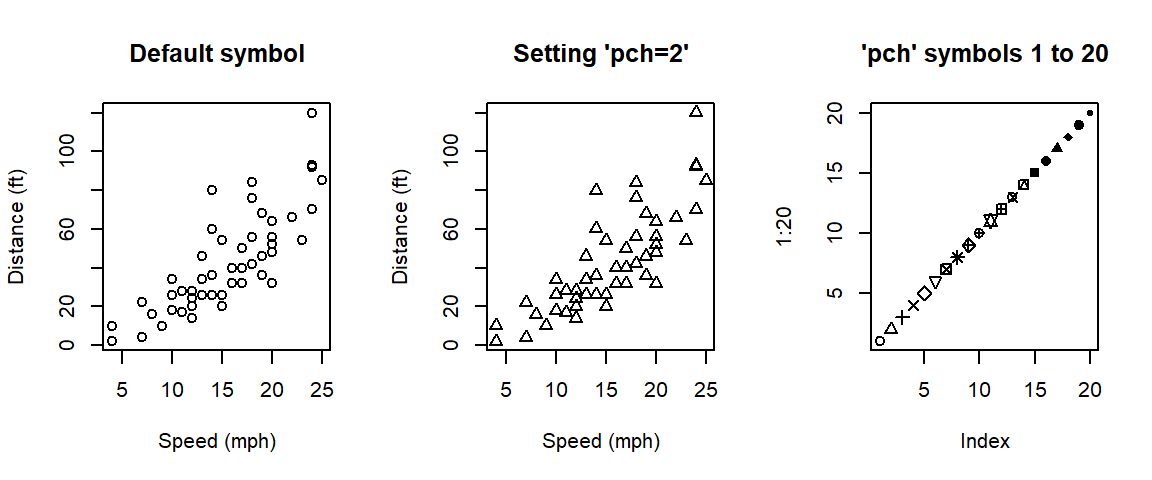
\includegraphics[width=1\linewidth,height=1\textheight]{_main_files/figure-latex/unnamed-chunk-12-1} \end{center}

\emph{Q1. Search the \texttt{plot} help page for `title', then add an appropriate title to your plot.}

\emph{Q2. \texttt{?points} opens the help page for points, search the help page for `pch' and change the symbol of your plot}

\emph{Q3. In relation to the cars dataset, plot stopping distance by speed, using indexing to show only those cars where speed\_mph\textgreater20}

\begin{Shaded}
\begin{Highlighting}[]
\FunctionTok{plot}\NormalTok{(dist\_ft }\SpecialCharTok{\textasciitilde{}}\NormalTok{ speed\_mph, }\AttributeTok{data =}\NormalTok{ cars2[cars2}\SpecialCharTok{$}\NormalTok{speed\_mph }\SpecialCharTok{\textgreater{}} \DecValTok{20}\NormalTok{, ], }
     \AttributeTok{xlab =} \StringTok{"Speed, mph"}\NormalTok{, }\AttributeTok{ylab =} \StringTok{"Distance, ft"}\NormalTok{, }\AttributeTok{pch =} \DecValTok{2}\NormalTok{)}
\end{Highlighting}
\end{Shaded}

\begin{center}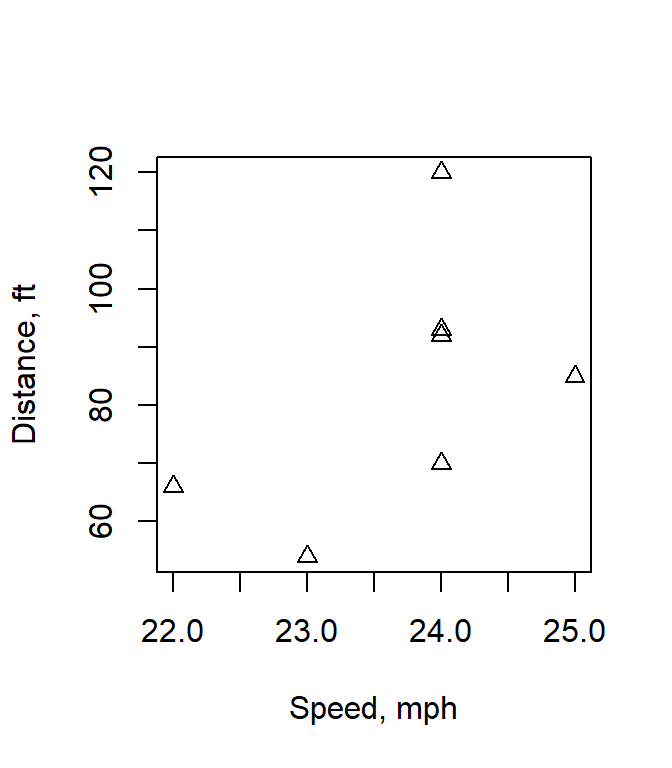
\includegraphics[width=0.4\linewidth,height=0.4\textheight]{_main_files/figure-latex/unnamed-chunk-14-1} \end{center}

\hypertarget{boxplots}{%
\subsection{Boxplots}\label{boxplots}}

Boxplots are used to summarise a continuous variable by levels of a factor. We will use the \texttt{mtcars} dataset to illustrate this.

Explore the dataframe using the code you've already covered. Which variables are categorical, which are continuous (or might be)?

\begin{Shaded}
\begin{Highlighting}[]
\FunctionTok{head}\NormalTok{(mtcars, }\DecValTok{2}\NormalTok{)}
\end{Highlighting}
\end{Shaded}

\begin{verbatim}
##               mpg cyl disp  hp drat    wt  qsec vs am gear carb
## Mazda RX4      21   6  160 110  3.9 2.620 16.46  0  1    4    4
## Mazda RX4 Wag  21   6  160 110  3.9 2.875 17.02  0  1    4    4
\end{verbatim}

\begin{Shaded}
\begin{Highlighting}[]
\FunctionTok{boxplot}\NormalTok{(mpg }\SpecialCharTok{\textasciitilde{}}\NormalTok{ cyl, }\AttributeTok{data =}\NormalTok{ mtcars)}
\end{Highlighting}
\end{Shaded}

\begin{figure}

{\centering 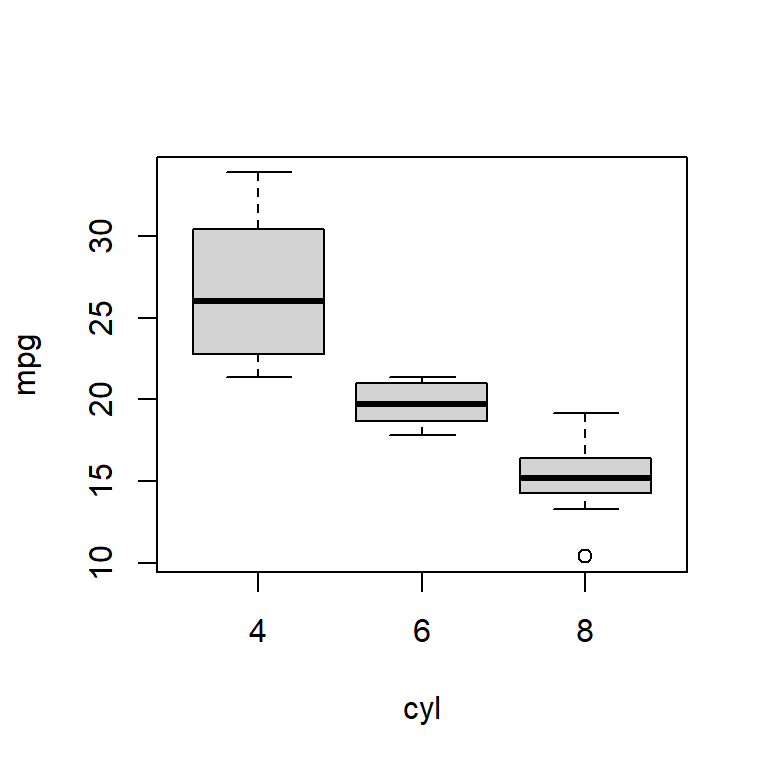
\includegraphics[width=0.5\linewidth,height=0.5\textheight]{_main_files/figure-latex/mplcyl-plot-1} 

}

\caption{Boxplot showing miles per litre vs. number of carburetors}\label{fig:mplcyl-plot}
\end{figure}

\begin{Shaded}
\begin{Highlighting}[]
\NormalTok{?boxplot}
\CommentTok{\# See examples at bottom of the help page}
\CommentTok{\# Produce a boxplot with axes labels and a title}
\end{Highlighting}
\end{Shaded}

Reproduce the plot shown in Fig. \ref{fig:mplcyl-plot} (assume 1 gallon = 4.5 L). Remember you can learn about these data with \texttt{?mtcars}. You will need to generate a new variable (miles per litre) and label your boxplot appropriately. You can limit the extent of the y-axis by adding the argument \texttt{ylim\ =\ c(a,\ b)} where \texttt{a} and \texttt{b} are the limits you want (e.g., \texttt{ylim\ =\ c(0,\ 100)}).

\emph{Q4. Use \texttt{?boxplot} to investigate what the box and whiskers in the boxplot acutally represent. Check you can reproduce the upper and lower adjacent values manually (see formula sheet)}

\hypertarget{line-plots}{%
\subsection{Line plots}\label{line-plots}}

Line plots are most often seen in time-series plots with time (e.g.~days or years etc) on the x-axis and the response on the y-axis. Line plots typically involve joining points with a line. The line can be straight or curved. Whatever the line is (which will be your choice), it indicates that you have made assumptions about the value of the response variable between successive measurements.

We will examine these plots using the dataset \texttt{lynx}, which consists of the number of Canadian lynx pelts sold per year between 1821 - 1934. It is a `classic' dataset as it shows a cyclical `boom-and-bust' lynx population (demonstrating predator-prey interactions).

First, we will create a variable \texttt{Year}.

\begin{Shaded}
\begin{Highlighting}[]
\FunctionTok{str}\NormalTok{(lynx)}
\end{Highlighting}
\end{Shaded}

\begin{verbatim}
##  Time-Series [1:114] from 1821 to 1934: 269 321 585 871 1475 ...
\end{verbatim}

\begin{Shaded}
\begin{Highlighting}[]
\FunctionTok{class}\NormalTok{(lynx) }\CommentTok{\# ts = time{-}series}
\NormalTok{lynx2 }\OtherTok{\textless{}{-}} \FunctionTok{as.data.frame}\NormalTok{(lynx) }
\FunctionTok{class}\NormalTok{(lynx2) }
\FunctionTok{head}\NormalTok{(lynx2, }\DecValTok{2}\NormalTok{) }
\NormalTok{lynx2}\SpecialCharTok{$}\NormalTok{Year }\OtherTok{\textless{}{-}} \FunctionTok{seq}\NormalTok{(}\AttributeTok{from =} \DecValTok{1821}\NormalTok{, }\AttributeTok{to =} \DecValTok{1934}\NormalTok{, }\AttributeTok{by =} \DecValTok{1}\NormalTok{)}
\end{Highlighting}
\end{Shaded}

In R, we use \emph{functions} to perform actions on \emph{objects} . Functions have arguments, taking the form \texttt{functionName(arg1=...,\ arg2=...)}. If you do not name the arguments, the function will assume that you are listing the arguments in order. See the help file with \texttt{?functionName} to see the argument order.

\emph{Q5. Using \texttt{seq()}, write a piece of code which generates odd numbers between 1 and 20 with and without specifying \texttt{from}, \texttt{to}, and \texttt{by}.}

\begin{Shaded}
\begin{Highlighting}[]
\CommentTok{\# change the name of the 1st column to \textquotesingle{}Trappings\textquotesingle{}}
\FunctionTok{names}\NormalTok{(lynx2)[}\DecValTok{1}\NormalTok{] }\OtherTok{\textless{}{-}} \StringTok{"Trappings"}
\FunctionTok{str}\NormalTok{(lynx2)}
\NormalTok{lynx2}\SpecialCharTok{$}\NormalTok{Trappings }\OtherTok{\textless{}{-}} \FunctionTok{as.numeric}\NormalTok{(lynx2}\SpecialCharTok{$}\NormalTok{Trappings) }\CommentTok{\# Time{-}Series is complicated.}
\FunctionTok{str}\NormalTok{(lynx2)}
\end{Highlighting}
\end{Shaded}

Use \texttt{?plot} to investigate options for plotting. Find the \texttt{type=} argument for plotting both the points and a connecting line. This might be the best option in this case. Why? Remind yourself the purpose of graphics.

\emph{Q6. Using the R plot function, produce a line plot of the Trappings data, as per Figure} \ref{fig:lynx-plot}\emph{.}

\begin{figure}

{\centering 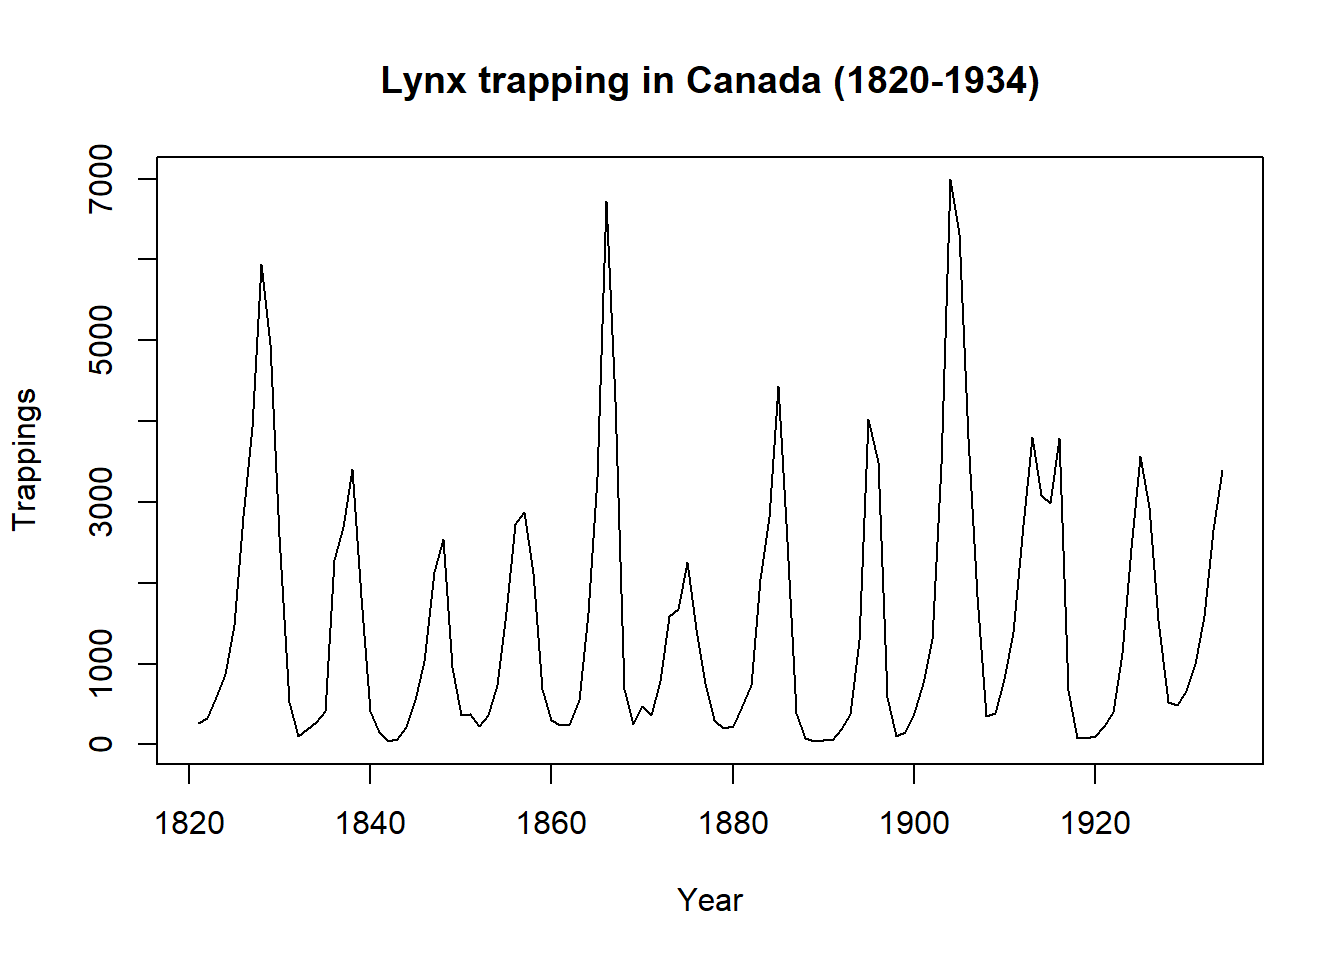
\includegraphics[width=0.5\linewidth,height=0.5\textheight]{_main_files/figure-latex/lynx-plot-1} 

}

\caption{The number of lynx trapped in Canada (1820-1934)}\label{fig:lynx-plot}
\end{figure}

Change the plot to show only the years up to 1900, then plot the Trappings on the log scale.

\hypertarget{histograms}{%
\subsection{Histograms}\label{histograms}}

Histograms are used to illustrate the distribution of continuous data. Histograms are often erroneously used to plot discrete data. In histograms the bars are adjacent (no gap) and this indicates that there is a continuum (i.e.~that the data are not discrete).

\begin{Shaded}
\begin{Highlighting}[]
\CommentTok{\# this gives very different information.}
\FunctionTok{hist}\NormalTok{(lynx2}\SpecialCharTok{$}\NormalTok{Trappings, }\AttributeTok{main =} \StringTok{"Lynx trapping"}\NormalTok{, }\AttributeTok{xlab =} \StringTok{"Trapped lynx per year"}\NormalTok{)}
\end{Highlighting}
\end{Shaded}

\begin{figure}

{\centering 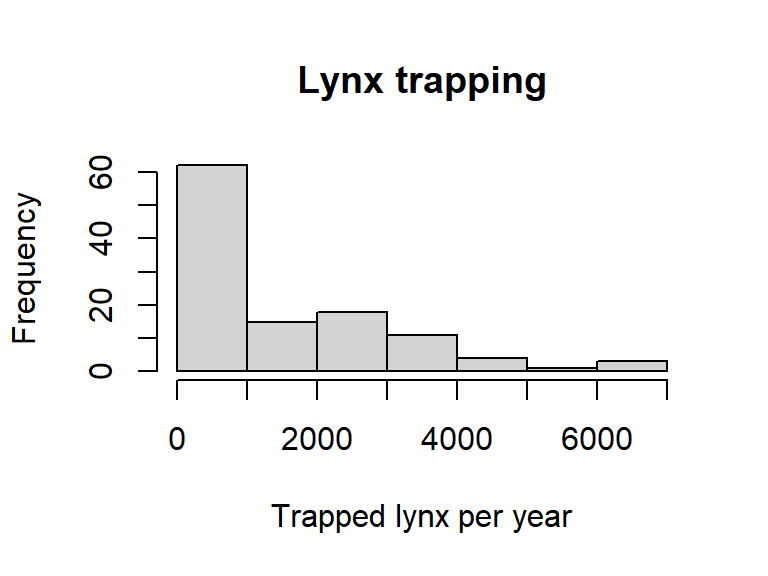
\includegraphics[width=0.5\linewidth,height=0.5\textheight]{_main_files/figure-latex/lynx-hist-default-1} 

}

\caption{Lynx pelts per year with default settings.}\label{fig:lynx-hist-default}
\end{figure}

Which range of values was most common across years?

Be aware that histograms can be quite sensitive to the bins that you use.

\begin{Shaded}
\begin{Highlighting}[]
\FunctionTok{par}\NormalTok{(}\AttributeTok{mfrow=}\FunctionTok{c}\NormalTok{(}\DecValTok{1}\NormalTok{,}\DecValTok{2}\NormalTok{)) }\CommentTok{\# panels for the plotting window}
\CommentTok{\# R takes the number of breaks as a suggestion}
\FunctionTok{hist}\NormalTok{(lynx2}\SpecialCharTok{$}\NormalTok{Trappings, }\AttributeTok{main =} \StringTok{"Lynx trapping"}\NormalTok{, }\AttributeTok{xlab =} \StringTok{"Trapped lynx per year"}\NormalTok{,}
     \AttributeTok{breaks =} \DecValTok{5}\NormalTok{)}
\CommentTok{\# this forces R to plot according to the defined breaks}
\FunctionTok{hist}\NormalTok{(lynx2}\SpecialCharTok{$}\NormalTok{Trappings,}
     \AttributeTok{main =} \StringTok{"Lynx trapping"}\NormalTok{, }\AttributeTok{xlab =} \StringTok{"Trapped lynx per year"}\NormalTok{,}
     \AttributeTok{breaks =} \FunctionTok{c}\NormalTok{(}\DecValTok{0}\NormalTok{, }\DecValTok{500}\NormalTok{, }\DecValTok{1000}\NormalTok{, }\DecValTok{2000}\NormalTok{, }\DecValTok{5000}\NormalTok{, }\DecValTok{10000}\NormalTok{))}
\end{Highlighting}
\end{Shaded}

\begin{figure}

{\centering 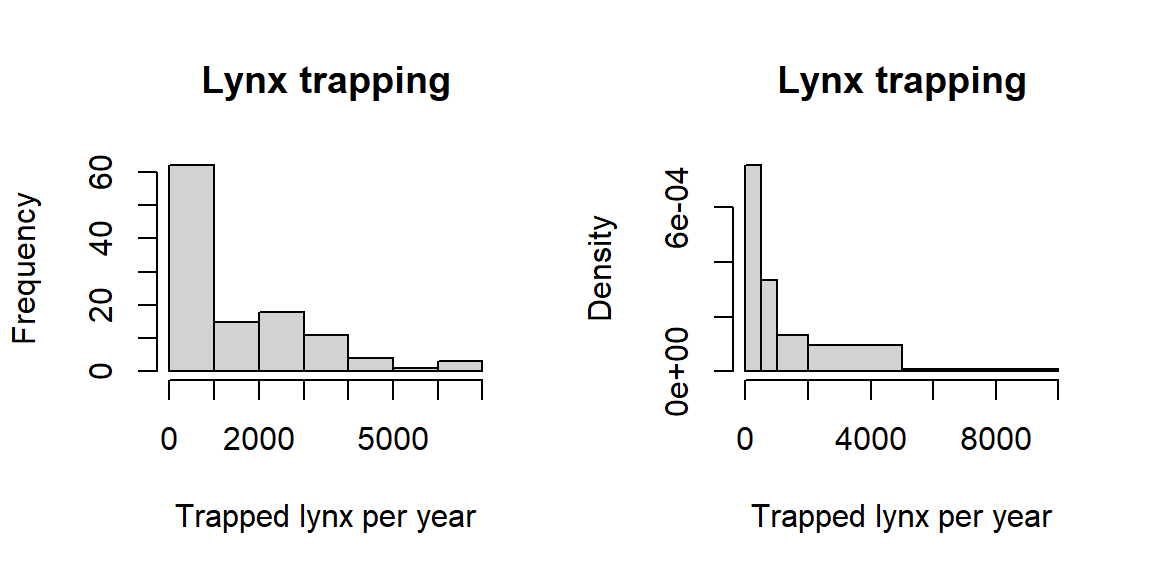
\includegraphics[width=0.8\linewidth,height=0.8\textheight]{_main_files/figure-latex/lynx-hist-b1-1} 

}

\caption{Lynx pelts per year with breaks=5 (left) and a vector of breaks (right).}\label{fig:lynx-hist-b1}
\end{figure}

\begin{Shaded}
\begin{Highlighting}[]
\FunctionTok{par}\NormalTok{(}\AttributeTok{mfrow =} \FunctionTok{c}\NormalTok{(}\DecValTok{2}\NormalTok{, }\DecValTok{2}\NormalTok{)) }\CommentTok{\# plot panels (2 rows x 2 columns)}
\FunctionTok{par}\NormalTok{(}\AttributeTok{mar =} \FunctionTok{rep}\NormalTok{(}\DecValTok{2}\NormalTok{, }\DecValTok{4}\NormalTok{)) }\CommentTok{\# change the plot margins}
\FunctionTok{hist}\NormalTok{(lynx2}\SpecialCharTok{$}\NormalTok{Trappings, }\AttributeTok{main =} \StringTok{"Plot 1"}\NormalTok{, }\AttributeTok{xlab =} \StringTok{"Trapped lynx per year"}\NormalTok{, }
     \AttributeTok{breaks =} \FunctionTok{seq}\NormalTok{(}\AttributeTok{from =} \DecValTok{0}\NormalTok{, }\AttributeTok{to =} \DecValTok{10000}\NormalTok{, }\AttributeTok{by =} \DecValTok{100}\NormalTok{))}
\FunctionTok{hist}\NormalTok{(lynx2}\SpecialCharTok{$}\NormalTok{Trappings, }\AttributeTok{main =} \StringTok{"Plot 2"}\NormalTok{, }\AttributeTok{xlab =} \StringTok{"Trapped lynx per year"}\NormalTok{, }
     \AttributeTok{breaks =} \FunctionTok{seq}\NormalTok{(}\AttributeTok{from =} \DecValTok{0}\NormalTok{, }\AttributeTok{to =} \DecValTok{10000}\NormalTok{, }\AttributeTok{by =} \DecValTok{500}\NormalTok{))}
\FunctionTok{hist}\NormalTok{(lynx2}\SpecialCharTok{$}\NormalTok{Trappings, }\AttributeTok{main =} \StringTok{"Plot 3"}\NormalTok{, }\AttributeTok{xlab =} \StringTok{"Trapped lynx per year"}\NormalTok{, }
     \AttributeTok{breaks =} \FunctionTok{seq}\NormalTok{(}\AttributeTok{from =} \DecValTok{0}\NormalTok{, }\AttributeTok{to =} \DecValTok{10000}\NormalTok{, }\AttributeTok{by =} \DecValTok{1000}\NormalTok{))}
\FunctionTok{hist}\NormalTok{(lynx2}\SpecialCharTok{$}\NormalTok{Trappings, }\AttributeTok{main =} \StringTok{"Plot 4"}\NormalTok{, }\AttributeTok{xlab =} \StringTok{"Trapped lynx per year"}\NormalTok{, }
     \AttributeTok{breaks =} \FunctionTok{seq}\NormalTok{(}\AttributeTok{from =} \DecValTok{0}\NormalTok{, }\AttributeTok{to =} \DecValTok{10000}\NormalTok{, }\AttributeTok{by =} \DecValTok{2000}\NormalTok{))}
\end{Highlighting}
\end{Shaded}

\begin{center}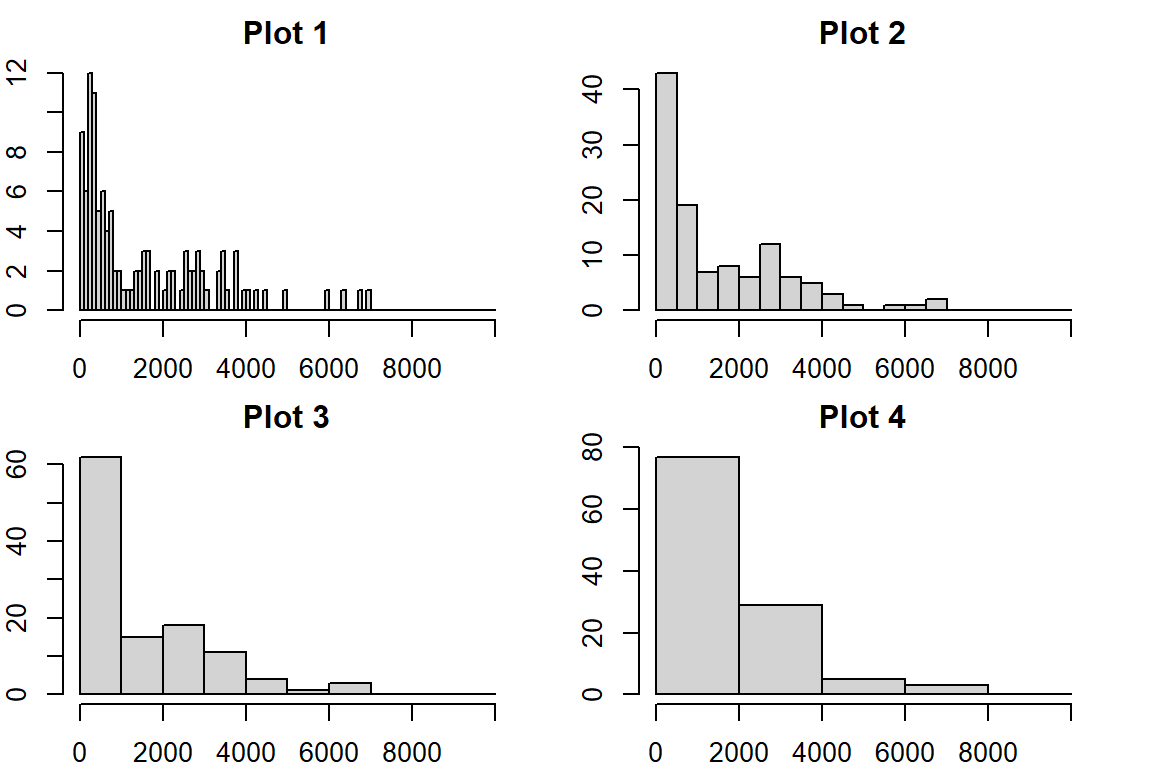
\includegraphics[width=0.8\linewidth,height=0.8\textheight]{_main_files/figure-latex/lynx-hist-panels-1} \end{center}

\begin{Shaded}
\begin{Highlighting}[]
\FunctionTok{par}\NormalTok{(}\AttributeTok{mfrow =} \FunctionTok{c}\NormalTok{(}\DecValTok{1}\NormalTok{, }\DecValTok{1}\NormalTok{)) }\CommentTok{\# reset the par setting.}
\end{Highlighting}
\end{Shaded}

Which of these plots is the most useful? There is no definitive answer to this, but Plot 1 is very busy and Plot 4 fails to show relevant detail near 0; Plot 2 or 3 communicate the patterns in the data most clearly.

As a general guideline, 5-15 breaks usually works well in a histogram.

\hypertarget{bar-graphs}{%
\subsection{Bar graphs}\label{bar-graphs}}

When you create a \texttt{data.frame} it defaults to naming the rows 1\ldots n, where n is the number of rows. \textbf{It is better practice to store relevant information in a column}, but you may occasionally come across a \texttt{data.frame} with row names. Converting between data types may lose this information.

Bar graphs are used to plot counts of categorical or discrete variables. We'll be using the \texttt{islands} dataset.

Working with data involves a lot of time spent tidying the datasets: cleaning, checking, and reshaping into useful formats. We will cover a more modern set of methods for this later in the course using the \emph{tidyverse} package. For now, we'll stay with base R. First, we need to tidy the \texttt{islands} data.

\begin{Shaded}
\begin{Highlighting}[]
\FunctionTok{str}\NormalTok{(islands) }
\FunctionTok{class}\NormalTok{(islands) }\CommentTok{\# this is a named numeric vector}
\FunctionTok{head}\NormalTok{(islands)}

\CommentTok{\# convert to a dataframe}
\NormalTok{islands.df }\OtherTok{\textless{}{-}} \FunctionTok{as.data.frame}\NormalTok{(islands) }
\FunctionTok{head}\NormalTok{(islands.df, }\DecValTok{2}\NormalTok{)}
\end{Highlighting}
\end{Shaded}

\begin{Shaded}
\begin{Highlighting}[]
\CommentTok{\# put the row names into a new column}
\NormalTok{islands.df}\SpecialCharTok{$}\NormalTok{LandMass }\OtherTok{\textless{}{-}} \FunctionTok{row.names}\NormalTok{(islands.df) }
\FunctionTok{head}\NormalTok{(islands.df, }\DecValTok{2}\NormalTok{)}
\end{Highlighting}
\end{Shaded}

\begin{verbatim}
##            islands   LandMass
## Africa       11506     Africa
## Antarctica    5500 Antarctica
\end{verbatim}

\begin{Shaded}
\begin{Highlighting}[]
\CommentTok{\# set row names to the row number}
\FunctionTok{row.names}\NormalTok{(islands.df) }\OtherTok{\textless{}{-}} \DecValTok{1}\SpecialCharTok{:}\FunctionTok{nrow}\NormalTok{(islands.df) }
\FunctionTok{names}\NormalTok{(islands.df)[}\DecValTok{1}\NormalTok{] }\OtherTok{\textless{}{-}} \StringTok{"Area"} 
\FunctionTok{head}\NormalTok{(islands.df, }\DecValTok{2}\NormalTok{) }
\end{Highlighting}
\end{Shaded}

\begin{verbatim}
##    Area   LandMass
## 1 11506     Africa
## 2  5500 Antarctica
\end{verbatim}

\begin{Shaded}
\begin{Highlighting}[]
\CommentTok{\# reorder by area}
\NormalTok{islands.df }\OtherTok{\textless{}{-}}\NormalTok{ islands.df[}\FunctionTok{order}\NormalTok{(islands.df}\SpecialCharTok{$}\NormalTok{Area, }\AttributeTok{decreasing =} \ConstantTok{TRUE}\NormalTok{), ]}
\FunctionTok{head}\NormalTok{(islands.df, }\DecValTok{3}\NormalTok{)}
\end{Highlighting}
\end{Shaded}

\begin{verbatim}
##     Area      LandMass
## 3  16988          Asia
## 1  11506        Africa
## 35  9390 North America
\end{verbatim}

We can use the function \texttt{barplot()} to plot the vector of island areas.

\begin{Shaded}
\begin{Highlighting}[]
\FunctionTok{par}\NormalTok{(}\AttributeTok{mar =} \FunctionTok{c}\NormalTok{(}\DecValTok{4}\NormalTok{, }\DecValTok{0}\NormalTok{, }\DecValTok{0}\NormalTok{, }\DecValTok{0}\NormalTok{)) }\CommentTok{\# change the margin sizes}
\FunctionTok{barplot}\NormalTok{(islands.df}\SpecialCharTok{$}\NormalTok{Area)}
\end{Highlighting}
\end{Shaded}

\begin{figure}

{\centering 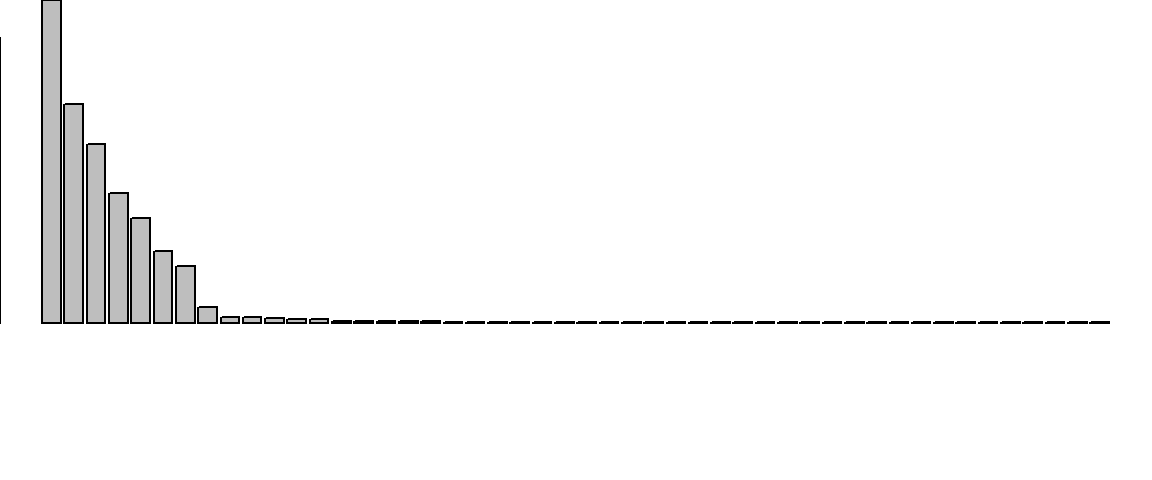
\includegraphics[width=0.8\linewidth,height=0.8\textheight]{_main_files/figure-latex/island-1-1} 

}

\caption{Island areas with barplot defaults}\label{fig:island-1}
\end{figure}

The whole dataset includes a lot of very small areas, so let's cut it down to just the 10 largest. Since the dataset is already sorted, we can take rows \texttt{1:10}.

\begin{Shaded}
\begin{Highlighting}[]
\FunctionTok{barplot}\NormalTok{(islands.df}\SpecialCharTok{$}\NormalTok{Area[}\DecValTok{1}\SpecialCharTok{:}\DecValTok{10}\NormalTok{])}
\end{Highlighting}
\end{Shaded}

\begin{figure}

{\centering 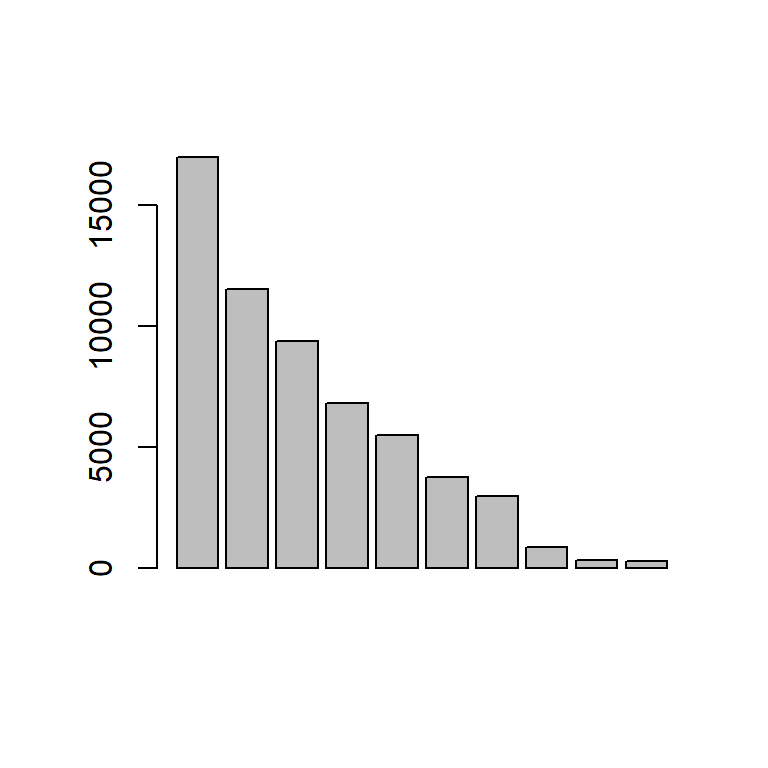
\includegraphics[width=0.5\linewidth,height=0.5\textheight]{_main_files/figure-latex/island-2-1} 

}

\caption{Top 10 island areas}\label{fig:island-2}
\end{figure}

And the next step is to add some names to the x-axis\ldots{}

\begin{Shaded}
\begin{Highlighting}[]
\FunctionTok{barplot}\NormalTok{(islands.df}\SpecialCharTok{$}\NormalTok{Area[}\DecValTok{1}\SpecialCharTok{:}\DecValTok{10}\NormalTok{], }\AttributeTok{names =}\NormalTok{ islands.df}\SpecialCharTok{$}\NormalTok{LandMass[}\DecValTok{1}\SpecialCharTok{:}\DecValTok{10}\NormalTok{])}
\end{Highlighting}
\end{Shaded}

\begin{figure}

{\centering 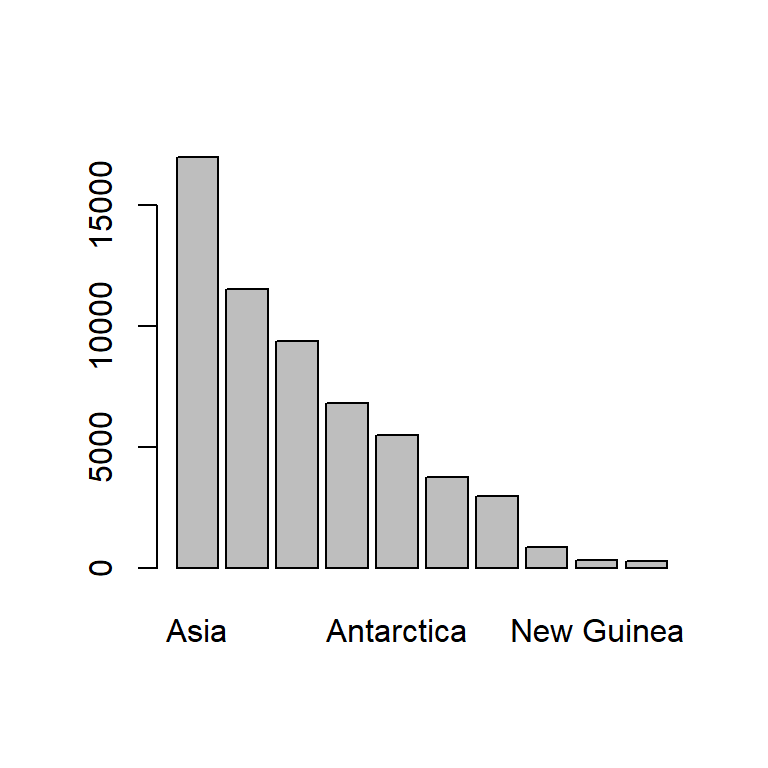
\includegraphics[width=0.5\linewidth,height=0.5\textheight]{_main_files/figure-latex/island-3-1} 

}

\caption{Top 10 island areas with names}\label{fig:island-3}
\end{figure}

Which of course are unreadable. The \texttt{las} argument (\texttt{?par}) controls how the axis labels relate to the axis line, so we can try adjusting that\ldots{}

\begin{Shaded}
\begin{Highlighting}[]
\FunctionTok{barplot}\NormalTok{(islands.df}\SpecialCharTok{$}\NormalTok{Area[}\DecValTok{1}\SpecialCharTok{:}\DecValTok{10}\NormalTok{], }\AttributeTok{names =}\NormalTok{ islands.df}\SpecialCharTok{$}\NormalTok{LandMass[}\DecValTok{1}\SpecialCharTok{:}\DecValTok{10}\NormalTok{], }\AttributeTok{las=}\DecValTok{3}\NormalTok{)}
\end{Highlighting}
\end{Shaded}

\begin{figure}

{\centering 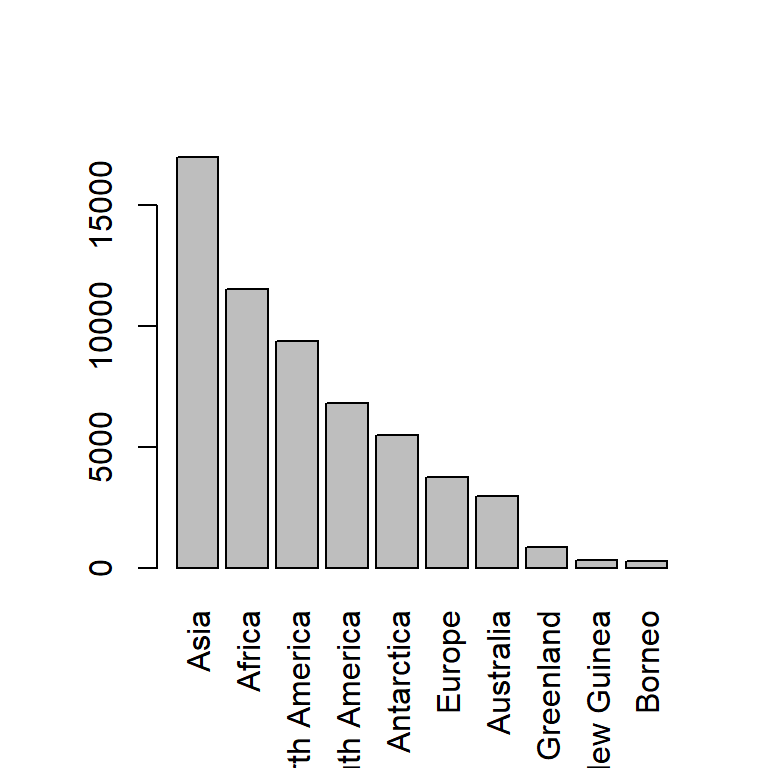
\includegraphics[width=0.5\linewidth,height=0.5\textheight]{_main_files/figure-latex/island-4-1} 

}

\caption{Top 10 island areas with names rotated}\label{fig:island-4}
\end{figure}

Maybe we just need to make the bars horizontal. To do this, we should adjust the margins again with \texttt{par(mar=...))}, set \texttt{horiz=TRUE}, and \texttt{las=1}, and use \texttt{{[}10:1{]}} so the largest is on top.

\begin{Shaded}
\begin{Highlighting}[]
\FunctionTok{par}\NormalTok{(}\AttributeTok{mar =} \FunctionTok{c}\NormalTok{(}\DecValTok{4}\NormalTok{, }\DecValTok{10}\NormalTok{, }\DecValTok{0}\NormalTok{, }\DecValTok{0}\NormalTok{))}
\FunctionTok{barplot}\NormalTok{(islands.df}\SpecialCharTok{$}\NormalTok{Area[}\DecValTok{10}\SpecialCharTok{:}\DecValTok{1}\NormalTok{], }\AttributeTok{names =}\NormalTok{ islands.df}\SpecialCharTok{$}\NormalTok{LandMass[}\DecValTok{10}\SpecialCharTok{:}\DecValTok{1}\NormalTok{], }
        \AttributeTok{horiz =} \ConstantTok{TRUE}\NormalTok{, }\AttributeTok{las =} \DecValTok{1}\NormalTok{, }\AttributeTok{xlab =} \StringTok{"Area (km2)"}\NormalTok{)}
\end{Highlighting}
\end{Shaded}

\begin{figure}

{\centering 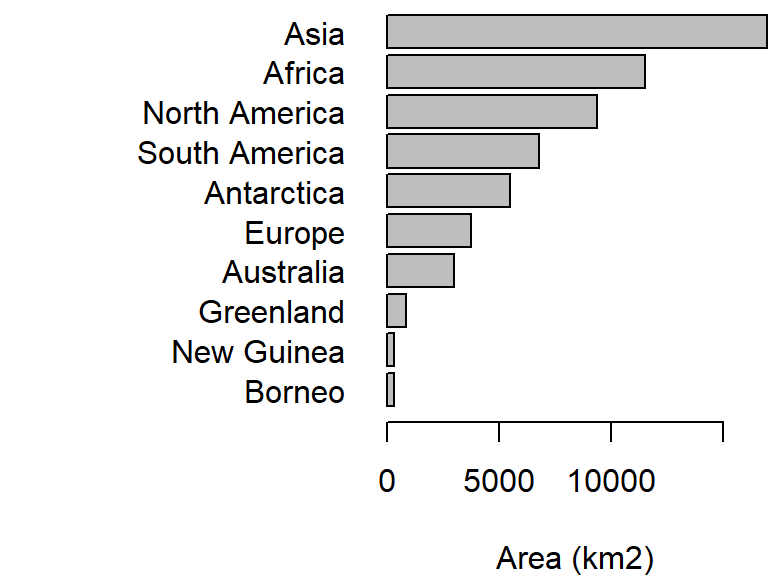
\includegraphics[width=0.5\linewidth,height=0.5\textheight]{_main_files/figure-latex/island-5-1} 

}

\caption{Finally! Did you know Antarctica is bigger than Europe?}\label{fig:island-5}
\end{figure}

As you may have noticed, visualization is an iterative process with lots of trial and error until you find a plot that communicates the message within the data well. There are several packages (e.g., \texttt{ggplot2}) that make these sort of adjustments and explorations less opaque than all of the options in \texttt{par()}.

\begin{center}\rule{0.5\linewidth}{0.5pt}\end{center}

\hypertarget{summary-statistics}{%
\section{Summary statistics}\label{summary-statistics}}

You will often need to summarise your data before you present it. Data summaries are usually contained in tables and they can replace graphics in certain situations, for example, where the data is relatively simple with a well understood distribution. There are numerous different types of summary statistics. Here we are concerned with central tendency and variability.

\emph{Q8. What are the three main measures of central tendency?}

\emph{Q9. What are three measures of variability?}

Different measures of central tendency and variability all have pros and cons and you need to be able to apply the most appropriate method to your data. Another summary statistic that you might include is sample size. R is very good at producing summary statistics, and there are myriad ways to produce them. We'll return to the \texttt{cars} dataset.

\begin{Shaded}
\begin{Highlighting}[]
\FunctionTok{summary}\NormalTok{(cars2) }
\end{Highlighting}
\end{Shaded}

\begin{verbatim}
##     dist_ft         speed_mph   
##  Min.   :  2.00   Min.   : 4.0  
##  1st Qu.: 26.00   1st Qu.:12.0  
##  Median : 36.00   Median :15.0  
##  Mean   : 42.98   Mean   :15.4  
##  3rd Qu.: 56.00   3rd Qu.:19.0  
##  Max.   :120.00   Max.   :25.0
\end{verbatim}

\begin{Shaded}
\begin{Highlighting}[]
\FunctionTok{summary}\NormalTok{(cars2[cars2}\SpecialCharTok{$}\NormalTok{speed\_mph }\SpecialCharTok{\textgreater{}} \DecValTok{20}\NormalTok{, ]) }
\end{Highlighting}
\end{Shaded}

\begin{Shaded}
\begin{Highlighting}[]
\CommentTok{\# There are several ways to access a column in a dataframe}
\FunctionTok{summary}\NormalTok{(cars2}\SpecialCharTok{$}\NormalTok{speed\_mph) }
\FunctionTok{summary}\NormalTok{(cars2[, }\DecValTok{2}\NormalTok{])}
\FunctionTok{summary}\NormalTok{(cars2[, }\StringTok{"speed\_mph"}\NormalTok{])}
\FunctionTok{summary}\NormalTok{(cars2[, }\FunctionTok{c}\NormalTok{(}\StringTok{"speed\_mph"}\NormalTok{, }\StringTok{"dist\_ft"}\NormalTok{)])}
\end{Highlighting}
\end{Shaded}

Often you'll wish to summarise your data across levels of certain factor. For example, levels of a certain treatment that you are applying. More complex summaries can be made using the \texttt{dplyr} package. We'll go into more detail later on some of the very powerful ways this package (and its friends in the \emph{tidyverse}) can be used.

First, you'll need to install it. The \emph{tidyverse} is a collection of packages. Install all of them with \texttt{install.packages("tidyverse")} (see Section @ref\{R\_intro\}).

We'll use the built-in dataset \texttt{InsectSprays}. Viewing your raw data can be an important check as well. You can open a spreadsheet-styled viewer in R using \texttt{View(YourDataFrame)}.

\begin{Shaded}
\begin{Highlighting}[]
\FunctionTok{str}\NormalTok{(InsectSprays)}
\end{Highlighting}
\end{Shaded}

\begin{verbatim}
## 'data.frame':    72 obs. of  2 variables:
##  $ count: num  10 7 20 14 14 12 10 23 17 20 ...
##  $ spray: Factor w/ 6 levels "A","B","C","D",..: 1 1 1 1 1 1 1 1 1 1 ...
\end{verbatim}

\begin{Shaded}
\begin{Highlighting}[]
\FunctionTok{glimpse}\NormalTok{(InsectSprays) }\CommentTok{\# glimpse() is loaded with tidyverse}
\end{Highlighting}
\end{Shaded}

\begin{verbatim}
## Rows: 72
## Columns: 2
## $ count <dbl> 10, 7, 20, 14, 14, 12, 10, 23, 17, 20, 14, 13, 11, 17, 21, 11, 1~
## $ spray <fct> A, A, A, A, A, A, A, A, A, A, A, A, B, B, B, B, B, B, B, B, B, B~
\end{verbatim}

\begin{Shaded}
\begin{Highlighting}[]
\CommentTok{\# spray is the categorical predictor; count is the response}
\FunctionTok{View}\NormalTok{(InsectSprays)}
\end{Highlighting}
\end{Shaded}

To do more complex summaries, we're going to string together a series of functions. This can be done in a nested format (e.g., \texttt{fun1(fun2(fun3(dataset)))}), but this gets unwieldy very quickly.

So, let's introduce the \emph{pipe} operator \texttt{\textbar{}\textgreater{}}. This takes the output from one function and feeds it as the first input of the next (e.g., \texttt{dataset\ \textbar{}\textgreater{}\ fun3()\ \textbar{}\textgreater{}\ fun2()\ \textbar{}\textgreater{}\ fun1()}), making code much more legible. Many functions in the \emph{tidyverse} are built for piping.

\begin{Shaded}
\begin{Highlighting}[]
\NormalTok{?}\StringTok{\textasciigrave{}}\AttributeTok{|\textgreater{}}\StringTok{\textasciigrave{}}
\end{Highlighting}
\end{Shaded}

\begin{Shaded}
\begin{Highlighting}[]
\CommentTok{\# use group\_by() with the grouping column name(s)}
\NormalTok{spray\_summaries }\OtherTok{\textless{}{-}}\NormalTok{ InsectSprays }\SpecialCharTok{|\textgreater{}}
  \FunctionTok{group\_by}\NormalTok{(spray) }\SpecialCharTok{|\textgreater{}}
  \FunctionTok{summarise}\NormalTok{(}\AttributeTok{count\_mean =} \FunctionTok{mean}\NormalTok{(count))}
\NormalTok{spray\_summaries}
\end{Highlighting}
\end{Shaded}

\begin{Shaded}
\begin{Highlighting}[]
\CommentTok{\# it is very easy to calculate any number of summary statistics}
\NormalTok{InsectSprays }\SpecialCharTok{|\textgreater{}}
  \FunctionTok{group\_by}\NormalTok{(spray) }\SpecialCharTok{|\textgreater{}}
  \FunctionTok{summarise}\NormalTok{(}\AttributeTok{mean =} \FunctionTok{mean}\NormalTok{(count) }\SpecialCharTok{|\textgreater{}} \FunctionTok{round}\NormalTok{(}\DecValTok{2}\NormalTok{),}
            \AttributeTok{median =} \FunctionTok{median}\NormalTok{(count),}
            \AttributeTok{max =} \FunctionTok{max}\NormalTok{(count),}
            \AttributeTok{sd =} \FunctionTok{sd}\NormalTok{(count) }\SpecialCharTok{|\textgreater{}} \FunctionTok{round}\NormalTok{(}\DecValTok{2}\NormalTok{),}
            \AttributeTok{N =} \FunctionTok{n}\NormalTok{(),}
            \AttributeTok{N\_over\_10 =} \FunctionTok{sum}\NormalTok{(count }\SpecialCharTok{\textgreater{}} \DecValTok{10}\NormalTok{))}
\end{Highlighting}
\end{Shaded}

\begin{verbatim}
## # A tibble: 6 x 7
##   spray  mean median   max    sd     N N_over_10
##   <fct> <dbl>  <dbl> <dbl> <dbl> <int>     <int>
## 1 A     14.5    14      23  4.72    12         9
## 2 B     15.3    16.5    21  4.27    12        11
## 3 C      2.08    1.5     7  1.98    12         0
## 4 D      4.92    5      12  2.5     12         1
## 5 E      3.5     3       6  1.73    12         0
## 6 F     16.7    15      26  6.21    12        10
\end{verbatim}

\hypertarget{which-measure-of-central-tendency-to-use}{%
\subsection{Which measure of central tendency to use}\label{which-measure-of-central-tendency-to-use}}

The choice of which measure of central tendency to use depends on the nature of the data and objectives of your research. However, there are some general rules. We will use datasets that you downloaded from Brightspace (Practicals \textgreater{} data). Remember to put these into the \emph{data} folder in your working directory (or modify the file paths in the code accordingly).

\begin{Shaded}
\begin{Highlighting}[]
\FunctionTok{library}\NormalTok{(readxl) }\CommentTok{\# installed with tidyverse, but not loaded in library(tidyverse)}
\CommentTok{\# this will load the \textquotesingle{}Scallop \%fat\textquotesingle{}data sheet from the xlsx spreadsheet.}
\NormalTok{scallop\_df }\OtherTok{\textless{}{-}} \FunctionTok{read\_excel}\NormalTok{(}\StringTok{"data/practical\_1.xlsx"}\NormalTok{, }\AttributeTok{sheet =} \StringTok{"Scallop \%fat"}\NormalTok{)}
\FunctionTok{str}\NormalTok{(scallop\_df)}
\end{Highlighting}
\end{Shaded}

\begin{verbatim}
## tibble [49 x 1] (S3: tbl_df/tbl/data.frame)
##  $ Scallop % fat: num [1:49] 22.5 24.1 18.2 32.5 17.4 23.6 21.5 22.2 27.6 22.2 ...
\end{verbatim}

\begin{Shaded}
\begin{Highlighting}[]
\CommentTok{\# avoid spaces and symbols in column names. It\textquotesingle{}s a pain.}
\FunctionTok{names}\NormalTok{(scallop\_df) }\OtherTok{\textless{}{-}} \StringTok{"fat\_pct"}
\end{Highlighting}
\end{Shaded}

\emph{Q10. Check the data using the methods above. Does it look OK to you?}

\emph{Q11. Are these data likely to be continuous or discontinuous?}

\emph{Q12. Create a plot to visualize the distribution of these data.}

\emph{Q13. Do you spot any issues?}

\begin{Shaded}
\begin{Highlighting}[]
\FunctionTok{hist}\NormalTok{(scallop\_df}\SpecialCharTok{$}\NormalTok{fat\_pct, }\AttributeTok{main =} \ConstantTok{NULL}\NormalTok{) }\CommentTok{\# (what does \textquotesingle{}main = NULL\textquotesingle{} do?)}
\end{Highlighting}
\end{Shaded}

\begin{center}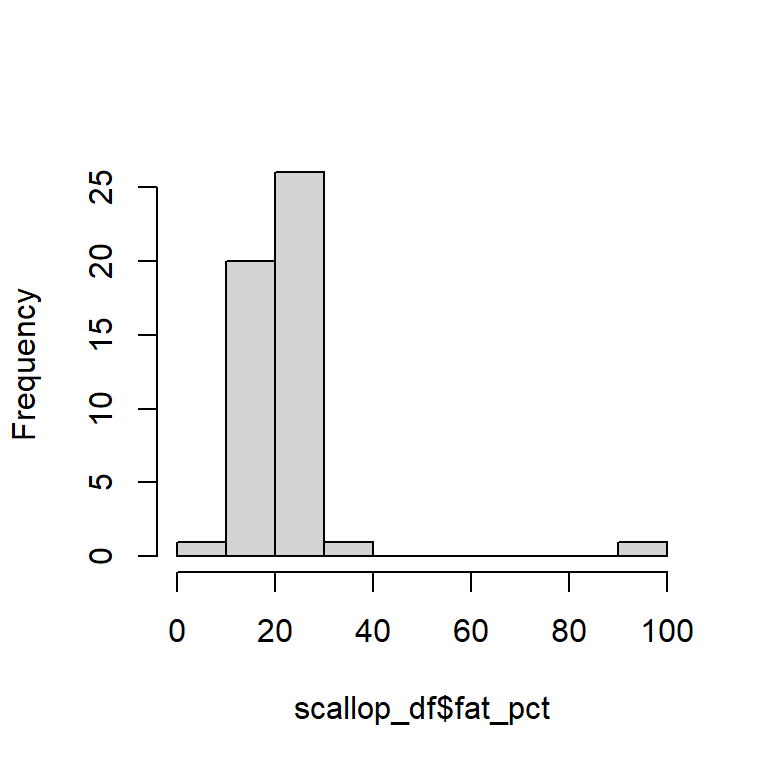
\includegraphics[width=0.5\linewidth,height=0.5\textheight]{_main_files/figure-latex/unnamed-chunk-32-1} \end{center}

You should have spotted a potential outlier. Data entry errors are very common, and a check against the original data sheet shows that the decimal was typed in the wrong place. The following code helps you ID which data entry is in error. We can now search for the `odd' observation i.e.~determine in which row the outlier is located.

\begin{Shaded}
\begin{Highlighting}[]
\FunctionTok{which}\NormalTok{(scallop\_df}\SpecialCharTok{$}\NormalTok{fat\_pct }\SpecialCharTok{\textgreater{}} \DecValTok{50}\NormalTok{) }
\end{Highlighting}
\end{Shaded}

\begin{verbatim}
## [1] 36
\end{verbatim}

\begin{Shaded}
\begin{Highlighting}[]
\NormalTok{scallop\_df}\SpecialCharTok{$}\NormalTok{fat\_pct[}\DecValTok{35}\SpecialCharTok{:}\DecValTok{37}\NormalTok{] }\CommentTok{\# row 36 is 99, but should be 9.9}
\end{Highlighting}
\end{Shaded}

\begin{verbatim}
## [1] 22.8 99.0 12.9
\end{verbatim}

\begin{Shaded}
\begin{Highlighting}[]
\NormalTok{scallop\_df }\OtherTok{\textless{}{-}}\NormalTok{ scallop\_df[, }\FunctionTok{c}\NormalTok{(}\DecValTok{1}\NormalTok{, }\DecValTok{1}\NormalTok{)] }\CommentTok{\# duplicate column}
\FunctionTok{names}\NormalTok{(scallop\_df) }\OtherTok{\textless{}{-}} \FunctionTok{c}\NormalTok{(}\StringTok{"fat\_pct\_orig"}\NormalTok{, }\StringTok{"fat\_pct\_corr"}\NormalTok{)}
\FunctionTok{head}\NormalTok{(scallop\_df, }\DecValTok{2}\NormalTok{)}
\end{Highlighting}
\end{Shaded}

\begin{verbatim}
## # A tibble: 2 x 2
##   fat_pct_orig fat_pct_corr
##          <dbl>        <dbl>
## 1         22.5         22.5
## 2         24.1         24.1
\end{verbatim}

\begin{Shaded}
\begin{Highlighting}[]
\CommentTok{\# there are many ways to \textquotesingle{}fix\textquotesingle{} the outlier in R.}
\CommentTok{\# You need to correct the outlier in row 36 of column \textquotesingle{}fat\_pct\_corr\textquotesingle{}}
\NormalTok{scallop\_df}\SpecialCharTok{$}\NormalTok{fat\_pct\_corr[}\DecValTok{36}\NormalTok{] }\OtherTok{\textless{}{-}} \FloatTok{9.9}
\FunctionTok{which}\NormalTok{(scallop\_df}\SpecialCharTok{$}\NormalTok{fat\_pct\_corr }\SpecialCharTok{\textgreater{}} \DecValTok{90}\NormalTok{) }
\CommentTok{\# integer(0) {-} this means that no elements in fat\_pct\_corr contain values \textgreater{}90}
\end{Highlighting}
\end{Shaded}

Now summarise \texttt{scallop\_df} using some of the methods above.

\emph{Q14. Create a histogram for the corrected column. How does it differ from the original column with the error?}

\emph{Q15. Calculate mean, variance, median, interquartile range, minimum, maximum and range for both fat\_pct\_orig and fat\_pct\_corr.}

\emph{Q16. Suppose the outlier was even bigger (i.e.~you typo was even worse). Adjust your data, multiplying the erroneous data item by 10; copy the `\_orig' column and change row 36 in that column to 999.}

\emph{Q17. Calculate the same summary statistics.}

\emph{Q18. Which measures of central tendency and variability are most `robust' against this outlier?}

Or look individually instead of calculating many metrics at once with \texttt{dplyr} functions:

\begin{Shaded}
\begin{Highlighting}[]
\FunctionTok{summary}\NormalTok{(scallop\_df}\SpecialCharTok{$}\NormalTok{fat\_pct\_corr)}
\end{Highlighting}
\end{Shaded}

\begin{verbatim}
##    Min. 1st Qu.  Median    Mean 3rd Qu.    Max. 
##    8.50   16.90   20.60   19.56   22.50   32.50
\end{verbatim}

\begin{Shaded}
\begin{Highlighting}[]
\FunctionTok{var}\NormalTok{(scallop\_df}\SpecialCharTok{$}\NormalTok{fat\_pct\_corr)}
\end{Highlighting}
\end{Shaded}

\begin{verbatim}
## [1] 22.79836
\end{verbatim}

\begin{Shaded}
\begin{Highlighting}[]
\FunctionTok{IQR}\NormalTok{(scallop\_df}\SpecialCharTok{$}\NormalTok{fat\_pct\_corr)}
\end{Highlighting}
\end{Shaded}

\begin{verbatim}
## [1] 5.6
\end{verbatim}

R is excellent at generating well formatted tables such as shown in Table \ref{tab:scallop-table}. What is missing from from Table \ref{tab:scallop-table}?

\begin{table}

\caption{\label{tab:scallop-table}Summary statistics with and without an outlier. Note which summary stats are most influenced by the outlier.}
\centering
\begin{tabular}[t]{lrrrrr}
\toprule
Column & Mean & Median & Standard deviation & Range & Interquartile range\\
\midrule
fat\_pct\_corr & 19.6 & 20.6 & 4.77 & 24.0 & 5.6\\
fat\_pct\_orig & 21.4 & 20.6 & 12.20 & 90.5 & 5.3\\
\bottomrule
\end{tabular}
\end{table}

\emph{Q19. How would the patterns seen in Table \ref{tab:scallop-table} influence your choice if you were required to summarise data that you thought might contain data that you weren't sure about? The three measure of central tendency are influenced to different extents by the `shape' of the data they are used to describe.}

\begin{Shaded}
\begin{Highlighting}[]
\NormalTok{hake\_df }\OtherTok{\textless{}{-}} \FunctionTok{read\_excel}\NormalTok{(}\StringTok{"data/practical\_1.xlsx"}\NormalTok{, }\AttributeTok{sheet =} \StringTok{"Hake"}\NormalTok{)}
\FunctionTok{str}\NormalTok{(hake\_df) }\CommentTok{\# once again, column names made for excel}
\end{Highlighting}
\end{Shaded}

\begin{verbatim}
## tibble [499 x 2] (S3: tbl_df/tbl/data.frame)
##  $ Year            : num [1:499] 1 1 1 1 1 1 1 1 1 1 ...
##  $ Hake length (mm): num [1:499] 190 219 181 148 206 204 168 197 178 211 ...
\end{verbatim}

\emph{Q20. What type of variable is \texttt{length}?}

\emph{Q21. Select an appropriate graphical method and display these data.}

\emph{Q22. In your own time, use the \texttt{dplyr} functions to summarise the hake data by year.}

\begin{Shaded}
\begin{Highlighting}[]
\NormalTok{hake\_df}\SpecialCharTok{$}\NormalTok{Year }\OtherTok{\textless{}{-}} \FunctionTok{as.factor}\NormalTok{(hake\_df}\SpecialCharTok{$}\NormalTok{Year) }\CommentTok{\# Treat as categorical, not numeric}
\FunctionTok{names}\NormalTok{(hake\_df) }\OtherTok{\textless{}{-}} \FunctionTok{c}\NormalTok{(}\StringTok{"Year"}\NormalTok{, }\StringTok{"Length"}\NormalTok{) }\CommentTok{\# simplify the column names}
\end{Highlighting}
\end{Shaded}

\begin{table}

\caption{\label{tab:hake-table}Summary of hake data.}
\centering
\begin{tabular}[t]{lr}
\toprule
Year & Mean length (cm)\\
\midrule
1 & 201.8\\
2 & 497.0\\
3 & 988.9\\
\bottomrule
\end{tabular}
\end{table}

Try to re-create Table \ref{tab:hake-table}.

The following `settling velocity' data relates to the settling velocity of salmon faecal material. Shona Magill generated these data.

\begin{Shaded}
\begin{Highlighting}[]
\FunctionTok{library}\NormalTok{(readxl)}
\NormalTok{fishPoo\_df }\OtherTok{\textless{}{-}} \FunctionTok{read\_excel}\NormalTok{(}\StringTok{"data/practical\_1.xlsx"}\NormalTok{, }\AttributeTok{sheet =} \StringTok{"Settling velocity"}\NormalTok{)}
\FunctionTok{str}\NormalTok{(fishPoo\_df)}
\end{Highlighting}
\end{Shaded}

\begin{verbatim}
## tibble [200 x 1] (S3: tbl_df/tbl/data.frame)
##  $ Settling velocity (mm s-1): num [1:200] 2.06 1.03 1.56 1.88 1.16 0.76 1.26 1.13 1.23 1.31 ...
\end{verbatim}

\emph{Q23. Produce a histogram of the settling velocity. Is it left or right skewed?}

\emph{Q24. Which measures of central tendency and variability are most appropriate?}

\emph{Q25. Sketch the distribution and indicate the relative positions of the mean and median.}

\emph{Q26. Generate a new column of the log-transformed settling velocity data and plot these data.}

\emph{Q27. What measures of central tendency and variability could be applied to the log-transformed data? Selecting the preferable measure of central tendency and variability in a dataset is not necessarily straightforward.}

Table 1.3 gives some indication of what issues you might consider.

\begin{table}

\caption{\label{tab:metric-table}Appropriate measures of central tendency and variability according to the underlying data distribution.}
\centering
\begin{tabular}[t]{lll}
\toprule
Data distribution & Central tendency metric & Variability metric\\
\midrule
Continuous,
unimodal,
symmetrical & Mean & Variance or sd\\
Continuous, skewed & Median & Interquartile range\\
Continuous,
multimodal & None; state modes & None; summarise by
group\\
Discontinuous & None; data-dependent & Range?\\
\bottomrule
\end{tabular}
\end{table}

\begin{center}\rule{0.5\linewidth}{0.5pt}\end{center}

\hypertarget{conclusions}{%
\section{Conclusions}\label{conclusions}}

Visualizing and summarising data are the critical first steps in the data analysis and reporting workflow. We use graphical methods to firstly explore our own data. Once we have made sense of it we select the most appropriate method to convey that understanding to our readers. We may help that communication by summarising data in the most appropriate way taking into account the distribution of the data and the presence of outliers.

\hypertarget{bin_pois}{%
\chapter{Binomial \& Poisson distributions}\label{bin_pois}}

The role of statisticians is often to determine the probability of events, or a series of events, occurring in nature given our current understanding of the processes that are involved (normally on the basis of previous data). This requires a mathematical description of a theoretical relationship. We refer to this as a statistical model. Statistical models are like any model (e.g.~a model aeroplane) in that they can be a useful simplification of reality. However, as George Box said, `all models are wrong but some are useful'. We will come back to this concept again and again throughout this course.

Two models, the binomial and Poisson distributions, often provide excellent approximations of real-world events. This means that they can be used to determine the likelihood of events or series of events given certain `reasonable' assumptions. In terms of planning, e.g.~in the insurance industry, this is extremely useful.

Examples of the questions addressed using the binomial and Poisson models include:

\begin{itemize}
\tightlist
\item
  How likely is it that four hurricanes hit the US in a single season based on historic data?
\item
  How likely is it that a `50-year' wave will hit in the next ten years? A 50 year wave is one of such size that it only occurs, on average, once in 50 years.
\item
  Is a river flooding now more than it used to? Is there a change in flooding frequency?
\item
  What proportion of clutches of fish eggs will contain all males?
\end{itemize}

This practical gives you the opportunity to practice using these distributions by hand and to use R to check that you get the answers correct. In the first part of this class you will conduct a number of short exercises to familiarise yourselves with the necessary commands in R to study probability using the binomial and Poisson distributions.

\begin{center}\rule{0.5\linewidth}{0.5pt}\end{center}

\hypertarget{the-binomial-distribution}{%
\section{The Binomial distribution}\label{the-binomial-distribution}}

\hypertarget{bernoulli-trials}{%
\subsection{Bernoulli trials}\label{bernoulli-trials}}

A Bernoulli trial is a single event with a \emph{binary} outcome (i.e., a success or a failure). Binary outcomes include:

\begin{itemize}
\tightlist
\item
  Alive / dead
\item
  Male / female
\item
  Pregnant / not pregnant
\item
  Guilty/ not guilty
\item
  Heads/tails
\item
  Win/lose
\end{itemize}

Things that can have more than two outcomes can be re-coded into two categories. This concept can be extended to numerous situations, such as:

\begin{itemize}
\tightlist
\item
  Income greater than £100,000 vs.~less than £100,000
\item
  Flower colour (blue vs.~not blue; red vs.~not red)
\end{itemize}

Each Bernoulli trial, by definition, is independent of all previous trials.

\emph{Q28. If you tossed a fair coin 99 times and each time it landed heads (and you weren't cheating), what is the probability of obtaining a head on the next toss of the coin?}

This is a different question from asking whether 100 heads or (99 heads + 1 tails) is more likely in a throw of 100 coins. This is different because these events are independent.

\hypertarget{the-binomial-distribution-1}{%
\subsection{The binomial distribution}\label{the-binomial-distribution-1}}

The binomial distribution is a discrete probability distribution that applies to a series of Bernoulli trials. For example, if you had 10 eggs under a (big) chicken and they were all female, you might wonder how likely this was by chance. If this kept happening, you might question whether something was somehow making the eggs female. Here, the outcome can be female or male, and the trial size is 10 (each egg is a `trial' with a binary outcome). You may question the assumption that the ratio female to male was 50:50 and favour an alternative hypothesis that the ratio was more female: less male. The binomial distribution allows you to quantify the probability of getting 10 females from 10 eggs (or any other number of females) for any given probability \(P(female)\). That is, we are not restricted to 50:50.

You need to know two things to use the binomial distribution. These are:

\begin{itemize}
\tightlist
\item
  the number of trials (\(n\), or sometimes \(k\))
\item
  probability of success (\(p\))
\end{itemize}

From \emph{p}, we can calculate the probability of failure as \(q = (1-p)\), since the two probabilities must sum to 1.

The distribution of a binomially distributed variable \(y\) is specified \(y \sim Binom(n,p)\). We denote \(P(x)\) as the probability of getting \(x\) successes where \(x\) is an integer \(0:n\).

The \textbf{mean of a binomial distribution} is \(n*p\). This gives you the \emph{expected} outcome. For example, if \(P(female)=0.5\) and \(n=10\) eggs the expected number of females is \(10*0.5=5\).

\hypertarget{binomial-distributions-by-hand}{%
\subsection{Binomial distributions by hand}\label{binomial-distributions-by-hand}}

Wongles always lay two eggs in a clutch but 50\% of the eggs are infertile and don't hatch. We are interested in the proportions that we can expect to hatch from one clutch (two eggs)

\emph{Q29. What is the event here?}

\emph{Q30. What is the probability of success?}

\emph{Q31. What is the number of trials?}

\emph{Q32. How many possible outcomes are there and what are they?}

\emph{Q33. Write down the model specification in the standard notation (with parameters)}

\emph{Q34. Calculate the expected proportions of clutches of eggs that contain two fertile, two infertile and one of each using the quadratic equation approach (i.e.~expand} \((p+q)^2\)\emph{).}

Often we are faced more than two events and the quadratic expansion approach you used above is no longer convenient. In such circumstances you use the binomial expression.

\emph{Q35. Copy down the binomial probability mass function (from \ref{appendix}) and use it as an alternative method for calculating the fertility proportions for two eggs (as per the quadratic equation approach).}

Oozle birds are much more sensible than Wongles and always have broods of eight offspring and all of them hatch. We are interested in modelling the probabilities of the proportion of male and female offspring in broods of eight eggs.

\emph{Q36. What is the Bernoulli event here (you are looking for something which has two mutually exclusive outcomes)?}

\emph{Q37. What are the theoretical limits to your outcomes (i.e, max numbers of each).}

\emph{Q38. What are the possible outcomes, and what is the total number of possible outcomes?}

\emph{Q39. Write down, in the standard manner, the model for Oozle egg gender (starting with} \(y \sim Binom(n,p)\)\emph{).}

We will assume that the probability (\(p\)) of any offspring being female is 0.5 and being male (\(q\)) is 0.5. For the extreme cases where all offspring are one sex, we can use simple probability theory: the probability of getting \(n\) females in a brood of size \(n\) is equal to \(p^n\).

\emph{Q40. Calculate the probability of obtaining eight male offspring.}

\emph{Q41. What is the mean number of females you would expect in Oozle broods?}

It gets more complicated when you want to know the probability of getting, say, 1 male and 7 females from your clutch of eight eggs.

\emph{Q42. Given that} \(p=q\)\emph{, what shape would expect the distribution to be?}

\emph{Q43. Use the Binomial expression (by hand) to calculate the probability of obtaining 0, 1, 2, 3, 4, 5, 6, 7 and 8 male offspring (note that the distribution is symmetrical).}

It is much easier, of course, to do this using R.

\hypertarget{binomial-distributions-in-r}{%
\subsection{Binomial distributions in R}\label{binomial-distributions-in-r}}

You can get probabilities for specific outcomes from a massive array of theoretical probability distributions from R. The binomial is just one of them and is implemented here.

\begin{Shaded}
\begin{Highlighting}[]
\NormalTok{num\_female }\OtherTok{\textless{}{-}} \DecValTok{4} \CommentTok{\# note that 4 is assigned to the variable called num\_female}
\NormalTok{num\_trials }\OtherTok{\textless{}{-}} \DecValTok{8}
\NormalTok{p\_female }\OtherTok{\textless{}{-}} \FloatTok{0.5}
\CommentTok{\# for a single probability: y\textasciitilde{}Binom(n=8, p=0.5) determine P(y\_i=4)}
\FunctionTok{paste0}\NormalTok{(}\StringTok{"P("}\NormalTok{, num\_female, }\StringTok{" female | "}\NormalTok{, num\_trials, }\StringTok{" eggs) = "}\NormalTok{,}
       \FunctionTok{dbinom}\NormalTok{(num\_female, num\_trials, p\_female))}
\end{Highlighting}
\end{Shaded}

\begin{verbatim}
## [1] "P(4 female | 8 eggs) = 0.2734375"
\end{verbatim}

\begin{Shaded}
\begin{Highlighting}[]
\FunctionTok{dbinom}\NormalTok{(}\DecValTok{4}\NormalTok{, }\DecValTok{8}\NormalTok{, }\FloatTok{0.5}\NormalTok{)}
\end{Highlighting}
\end{Shaded}

Often we want to know cumulative probabilities. This allows us to answer the question, for example, of what is the probability of obtaining \textless{} 4 females in a brood of 8 eggs. Here, \textless4 equates to the cumulative probability P(0) + P(1) + P(2) + P(3).

\begin{Shaded}
\begin{Highlighting}[]
\CommentTok{\# pbinom gives the cumulative probability}
\FunctionTok{paste}\NormalTok{(}\StringTok{"The cumulative probability is"}\NormalTok{, }
      \FunctionTok{max}\NormalTok{(}\FunctionTok{pbinom}\NormalTok{(}\DecValTok{0}\SpecialCharTok{:}\NormalTok{num\_female }\SpecialCharTok{{-}} \DecValTok{1}\NormalTok{, num\_trials, p\_female)))}
\end{Highlighting}
\end{Shaded}

\begin{verbatim}
## [1] "The cumulative probability is 0.36328125"
\end{verbatim}

\emph{Q44. Why do we parameterise \texttt{pbinom()} with \texttt{num\_female-1} rather than \texttt{num\_female}?}

\emph{Q45. Would this change if the question was} \(P( \leq 4)\)\emph{?}

\emph{Q46. Take the 'max'out of the above line and run again. You should see 5 cumulative probabilities. Why is the first cumulative probability zero?}

\emph{Q47. Calculate P(\textless{} 4 females \textbar{} 8 eggs) using \texttt{dbinom()} instead of \texttt{pbinom()}.}

\begin{Shaded}
\begin{Highlighting}[]
\CommentTok{\# You can check what R is doing by running parts of code:}
\DecValTok{0}\SpecialCharTok{:}\NormalTok{num\_female }\SpecialCharTok{{-}} \DecValTok{1} \CommentTok{\# is this what you expected?}
\end{Highlighting}
\end{Shaded}

\begin{verbatim}
## [1] -1  0  1  2  3
\end{verbatim}

\begin{Shaded}
\begin{Highlighting}[]
\DecValTok{0}\SpecialCharTok{:}\NormalTok{(num\_female }\SpecialCharTok{{-}} \DecValTok{1}\NormalTok{) }\CommentTok{\# this is actually what we want.}
\end{Highlighting}
\end{Shaded}

\begin{verbatim}
## [1] 0 1 2 3
\end{verbatim}

\begin{Shaded}
\begin{Highlighting}[]
\CommentTok{\# Correct the code above. Why did this bug have no effect?}
\end{Highlighting}
\end{Shaded}

\emph{Q48. What is the probability of getting 3 females?}

\emph{Q49. What is the probability of getting 8 females?}

\emph{Q50. What cumulative probabilities would you need to consider to answer the question `What is the probability of getting fewer than three females?'}

\emph{Q51. Write down the model that describes this random process (number of females per eight eggs). Your answer should be like this: }\(y \sim Binom(n, p)\)\emph{.}

\emph{Q52. What is the probability of getting \textless{} 4 females?}

\emph{Q53. What is the probability of getting \(\leq\) 4 females?}

\emph{Q54. What is the probability of getting \textgreater{} than 8 females?}

\emph{Q55. What is the probability of getting \(\geq\) than 2 females?}

Let's visualise these distributions in order to better understand them.

\begin{Shaded}
\begin{Highlighting}[]
\CommentTok{\# Run this, then explore values of p\_female}
\CommentTok{\# Note: \textquotesingle{}success\textquotesingle{} and \textquotesingle{}failure\textquotesingle{} is arbitrary. Just make sure you\textquotesingle{}re calculating}
\CommentTok{\# what you think. How would you calculate the probabilities for males instead?}
\NormalTok{num\_female }\OtherTok{\textless{}{-}} \FunctionTok{seq}\NormalTok{(}\DecValTok{0}\NormalTok{, }\DecValTok{8}\NormalTok{) }
\NormalTok{p\_female }\OtherTok{\textless{}{-}} \FloatTok{0.5} \CommentTok{\# what are the limits of p\_female?}
\NormalTok{prFemale\_df }\OtherTok{\textless{}{-}} \FunctionTok{data.frame}\NormalTok{(}\AttributeTok{num\_female =}\NormalTok{ num\_female, }
                          \AttributeTok{prob =} \FunctionTok{dbinom}\NormalTok{(num\_female, }\FunctionTok{max}\NormalTok{(num\_female), p\_female)) }
\NormalTok{prFemale\_df }
\end{Highlighting}
\end{Shaded}

\begin{verbatim}
##   num_female       prob
## 1          0 0.00390625
## 2          1 0.03125000
## 3          2 0.10937500
## 4          3 0.21875000
## 5          4 0.27343750
## 6          5 0.21875000
## 7          6 0.10937500
## 8          7 0.03125000
## 9          8 0.00390625
\end{verbatim}

\begin{Shaded}
\begin{Highlighting}[]
\FunctionTok{barplot}\NormalTok{(prFemale\_df}\SpecialCharTok{$}\NormalTok{prob, }\AttributeTok{names =}\NormalTok{ prFemale\_df}\SpecialCharTok{$}\NormalTok{num\_female, }
        \AttributeTok{xlab =} \StringTok{"Number of females"}\NormalTok{, }\AttributeTok{ylab =} \StringTok{"Probability"}\NormalTok{)}
\end{Highlighting}
\end{Shaded}

\begin{center}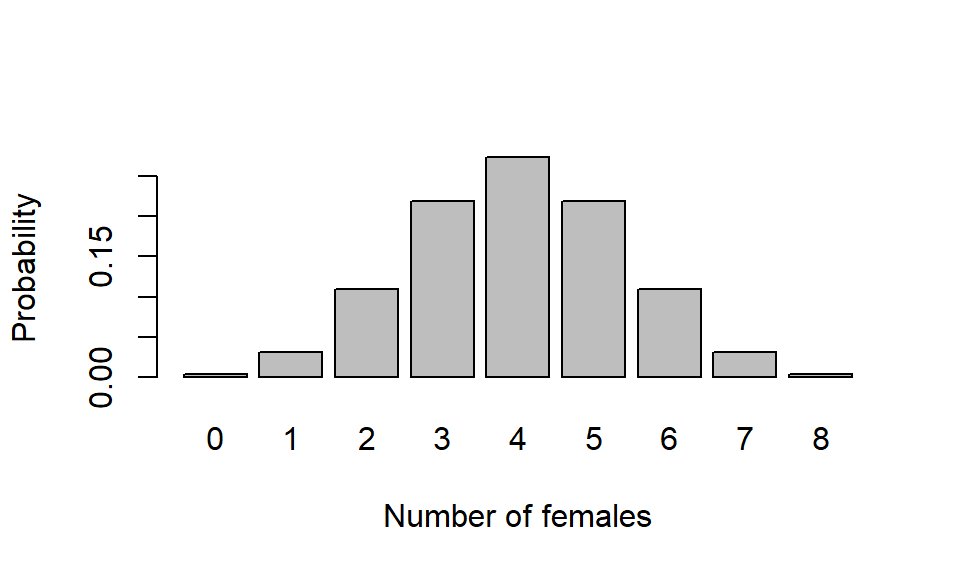
\includegraphics[width=0.5\linewidth,height=0.5\textheight]{_main_files/figure-latex/unnamed-chunk-43-1} \end{center}

\begin{Shaded}
\begin{Highlighting}[]
\NormalTok{prFemale\_df}\SpecialCharTok{$}\NormalTok{cumul\_prob }\OtherTok{\textless{}{-}} \FunctionTok{cumsum}\NormalTok{(prFemale\_df}\SpecialCharTok{$}\NormalTok{prob)}
\FunctionTok{barplot}\NormalTok{(prFemale\_df}\SpecialCharTok{$}\NormalTok{cumul\_prob, }\AttributeTok{names =}\NormalTok{ prFemale\_df}\SpecialCharTok{$}\NormalTok{num\_female, }
        \AttributeTok{xlab =} \StringTok{"Enter the correct label!"}\NormalTok{, }\AttributeTok{ylab =} \StringTok{"Enter the correct label!"}\NormalTok{)}
\end{Highlighting}
\end{Shaded}

\begin{center}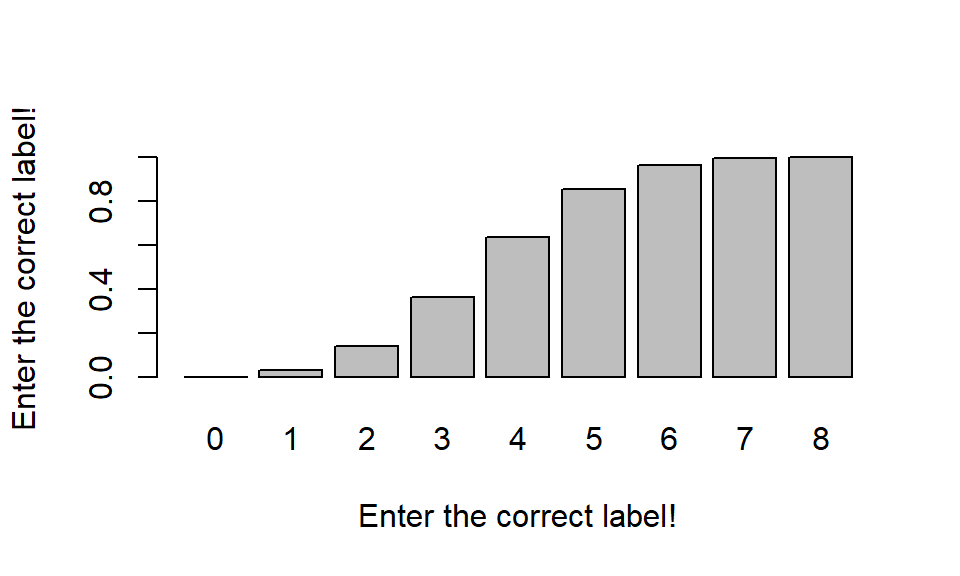
\includegraphics[width=0.5\linewidth,height=0.5\textheight]{_main_files/figure-latex/unnamed-chunk-44-1} \end{center}

Try re-plotting so that the two panels appear side by side (hint: \texttt{par(mfrow=c(...))}).

Note \(P(y_i=x)\) is read as `the probability that a random observation \(y_i\) equals \(x\)'. Sometimes this includes conditions: \(P(y_i=x|n,p)\), which is read as the probability that \(y_i\) equals \(x\) given \(n\) and \(p\). You may instead see \(P()\), \(Pr()\), \(p()\), or \(Prob()\). The interpretation of \(P(y_i=8\ |\ n=8,\ p=0.5)\) is that the probability of 8 female offspring is 0.00391. So, if we have 500 broods, each with 8 eggs, we expect \(500 * 0.00391 = 1.95 \approx 2\) broods to be all female.

\emph{Q56. Why is a bargraph the appropriate plot here?}

\emph{Q57. What do you notice about the shape of the distribution when \(p=q=0.5\)?}

\emph{Q58. Re-run the analysis with the probability of female as 0.8. Plot the results.}

\emph{Q59. What is the shape of the distribution now?}

\begin{center}\rule{0.5\linewidth}{0.5pt}\end{center}

\hypertarget{the-poisson-distribution}{%
\section{The Poisson distribution}\label{the-poisson-distribution}}

The Poisson distribution is another probability distribution that describes discrete events that occur in space and/or time. The Poisson distribution is used to model (predict) the distribution of events that are rare, random, and independent. This can include events like earthquakes, storms, or the number of bends arriving at the SAMS recompression facility.

The Poisson distribution takes a single parameter: the mean. If a variable is Poisson distributed, its variance will equal its mean. This is a diagnostic feature of the distribution. The Poisson distribution is a discrete probability distribution, but its parameter, the mean, is continuous (similar to continuous \(p\) for the discrete binomial distribution).

The Poisson formula is simple - copy it from \ref{appendix} into here:
\newline
\newline
\newline
\newline
\newline
\newline
\newline
\(\bar{y}\) is the mean, \(x\) is the outcome of interest, \(e\) is Euler's number, and \(!\) is factorial.

\hypertarget{poisson-distributions-by-hand}{%
\subsection{Poisson distributions by hand}\label{poisson-distributions-by-hand}}

These problems usually start by asking you to calculate the mean number of observations made per unit of space or time. This is the Poisson parameter, and is referred to as the \emph{rate} or as \emph{lambda} (\(\lambda\)). The unit could be spatial (e.g., per \(m^2\)) or temporal (e.g., per hour or day).

Consider randomly throwing 1\(m^2\) quadrat- on a sandy beach covered in worm casts, as illustrated in Fig. \ref{fig:worm-casts}. You then count the number of casts in each quadrat.

\begin{figure}
\centerline{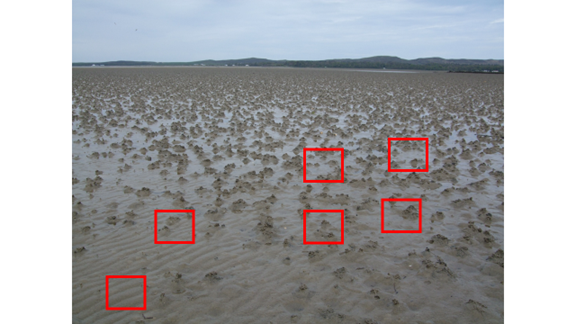
\includegraphics[width=0.5\textwidth]{figs/worm_casts.png}}
\caption{Worm casts on a sandy beach with 1x1 m quadrats.}
\label{fig:worm-casts}
\end{figure}

From these data you can calculate the mean number of observations per unit.

The code below generates a dataframe from which you can determine that the mean number of worms per quadrat is 1.41. We wish to predict the proportion of quadrats that would contain 0, 1, 2, 3, 4, and 5 worms, assuming that the worms are independently distributed across space (i.e., random: one worm's location has no effect on another worm's location, and there is no relevant environmental variation).

We thus wish to determine the probability of observing our data assuming that the worms casts are randomly distributed. To do this, we need to know the probability of observing each count (zero to infinity), given the mean count per quadrat.

\begin{Shaded}
\begin{Highlighting}[]
\CommentTok{\# num\_worms is the number of worms per quadrat}
\CommentTok{\# num\_quadrats is numbers of quadrats observed containing that number of worms}
\CommentTok{\# this dataset is summarised. Raw data might have columns: quadrat\_id, num\_worms}
\NormalTok{worm\_df }\OtherTok{\textless{}{-}} \FunctionTok{data.frame}\NormalTok{(}\AttributeTok{num\_worms =} \FunctionTok{c}\NormalTok{(}\DecValTok{0}\NormalTok{, }\DecValTok{1}\NormalTok{, }\DecValTok{2}\NormalTok{, }\DecValTok{3}\NormalTok{, }\DecValTok{4}\NormalTok{, }\DecValTok{5}\NormalTok{, }\DecValTok{6}\NormalTok{),}
                      \AttributeTok{num\_quadrats =} \FunctionTok{c}\NormalTok{(}\DecValTok{35}\NormalTok{, }\DecValTok{28}\NormalTok{, }\DecValTok{15}\NormalTok{, }\DecValTok{10}\NormalTok{, }\DecValTok{7}\NormalTok{, }\DecValTok{5}\NormalTok{, }\DecValTok{0}\NormalTok{))}
\NormalTok{worm\_df }\CommentTok{\# display dataframe}
\end{Highlighting}
\end{Shaded}

\begin{verbatim}
##   num_worms num_quadrats
## 1         0           35
## 2         1           28
## 3         2           15
## 4         3           10
## 5         4            7
## 6         5            5
## 7         6            0
\end{verbatim}

As the number of worms per quadrat is low compared to the number of worms that could exist within a quadrat we consider these are rare events and hence can be (reasonably) described by a Poisson distribution (assuming they are independent).

From just the mean we are able to calculate the expected frequency of observing different number of worms in any quadrat (assuming the model assumptions are met - remind yourself what these assumptions are). The number of worms per quadrat (\(y\)) is discrete; it can only take integers greater or equal to zero.

Probability questions often includes terms such as \(P(y_i \leq a)\). That is, the probability that an observation \(i\) of the random variable \(y\) is less than or equal to \(a\). For example, in this context you might get asked for \(P(y_i \leq 1)\) which asks what is the probability of a random quadrat being thrown (\(y_i\)) containing less or equal to 1 worm cast (\(a\), an integer value). To be fully complete, we might even write \(P(y_i \leq 1 | \lambda)\), which acknowledges that we know the (sample) mean.

So, if you are interested in predicting the probability of obtaining 1 or fewer worms per quadrat, you would start your calculation by writing \(P(y_i = 0) + P(y_i=1) = \dots\).

\emph{Q60. Use the Poisson formula to calculate the expected frequency of 0, 1 \& 2 worms per quadrat.}

\emph{Q61. What calculation would you need to conduct to determine }\(P(y_i \geq 1)\)\emph{?}

Again, calculating Poisson distributed variables in R is easier than doing it by hand, but you must be sure of what you are actually asking (hence bothering with the hand calculations).

\hypertarget{poisson-distributions-in-r}{%
\subsection{Poisson distributions in R}\label{poisson-distributions-in-r}}

You can determine the expected probabilities for each worm count per quadrat once you have determined the mean count of worms per quadrat. Since we have a summarised dataset (i.e., the number of observations \texttt{num\_quadrats} for each number of worms \texttt{num\_worms}, rather than the raw data with a row for each quadrat), we need to do some basic calculations. The mean number of worms per quadrat = (total number of worms) / (total number of quadrats).

\begin{Shaded}
\begin{Highlighting}[]
\FunctionTok{sum}\NormalTok{(worm\_df}\SpecialCharTok{$}\NormalTok{num\_quadrats) }\CommentTok{\# total number of quadrats}
\end{Highlighting}
\end{Shaded}

\begin{verbatim}
## [1] 100
\end{verbatim}

\begin{Shaded}
\begin{Highlighting}[]
\NormalTok{lambda\_worms }\OtherTok{\textless{}{-}} \FunctionTok{with}\NormalTok{(worm\_df, }\FunctionTok{sum}\NormalTok{(num\_worms }\SpecialCharTok{*}\NormalTok{ num\_quadrats) }\SpecialCharTok{/} \FunctionTok{sum}\NormalTok{(num\_quadrats))}
\FunctionTok{paste}\NormalTok{(}\StringTok{"The mean is"}\NormalTok{, lambda\_worms, }\StringTok{"worms per quadrat"}\NormalTok{)}
\end{Highlighting}
\end{Shaded}

\begin{verbatim}
## [1] "The mean is 1.41 worms per quadrat"
\end{verbatim}

Interpreting typical questions: taking \(P(y_i \leq a)\), when \(a=5\) and you are asked to determine \(P(y_i \leq 5)\), what you are being asked is ``What is the probability of a random quadrat (\(y_i\)) containing five or fewer worms?''. In order to determine this, you need to know the mean number per quadrat. When the mean number is 1.41 worms per quadrat, \(P(y_i \leq 5) = 0.997\) (3 sf). This means that, if your data are Poisson distributed, it is highly likely that there will be fewer than five worms in your quadrat if \(\lambda = 1.41\).

\emph{Q62. If the mean number of worms was 3 per quadrat, would you be more or less likely to get five worms in your quadrat?}

Needless to say, you can use R to calculate Poisson probabilities. Starting with a simple example:

\begin{Shaded}
\begin{Highlighting}[]
\CommentTok{\# ?dpois }
\CommentTok{\# for questions like \textquotesingle{}determine P(y\_i=a | lambda)\textquotesingle{}}
\NormalTok{a }\OtherTok{\textless{}{-}} \DecValTok{5} 
\NormalTok{lambda }\OtherTok{\textless{}{-}} \FloatTok{1.41} 
\FunctionTok{dpois}\NormalTok{(a, lambda) }\CommentTok{\# probability of observing \textquotesingle{}a\textquotesingle{} worms per quadrat: dpois()}
\end{Highlighting}
\end{Shaded}

\begin{verbatim}
## [1] 0.01133859
\end{verbatim}

\begin{Shaded}
\begin{Highlighting}[]
\FunctionTok{ppois}\NormalTok{(a, lambda) }\CommentTok{\# probability of observing \textgreater{}= \textquotesingle{}a\textquotesingle{} worms: ppois()}
\end{Highlighting}
\end{Shaded}

\begin{verbatim}
## [1] 0.9966869
\end{verbatim}

\begin{Shaded}
\begin{Highlighting}[]
\DocumentationTok{\#\# ppois(0:a, lambda) \# what does 0:a mean? What\textquotesingle{}s another way to do this?}
\FunctionTok{signif}\NormalTok{(}\FunctionTok{ppois}\NormalTok{(}\DecValTok{0}\SpecialCharTok{:}\NormalTok{a, lambda), }\DecValTok{3}\NormalTok{) }\CommentTok{\# round with ?signif}
\end{Highlighting}
\end{Shaded}

\begin{verbatim}
## [1] 0.244 0.588 0.831 0.945 0.985 0.997
\end{verbatim}

\begin{Shaded}
\begin{Highlighting}[]
\FunctionTok{barplot}\NormalTok{(}\FunctionTok{dpois}\NormalTok{(}\DecValTok{0}\SpecialCharTok{:}\NormalTok{a, lambda),}
        \AttributeTok{ylab =} \StringTok{"Probability"}\NormalTok{, }\AttributeTok{xlab =} \StringTok{"Number of worms"}\NormalTok{,}
        \AttributeTok{space =} \FloatTok{0.2}\NormalTok{, }\AttributeTok{ylim =} \FunctionTok{c}\NormalTok{(}\DecValTok{0}\NormalTok{, }\FloatTok{0.5}\NormalTok{), }\AttributeTok{names.arg =} \DecValTok{0}\SpecialCharTok{:}\NormalTok{a)}
\end{Highlighting}
\end{Shaded}

\begin{center}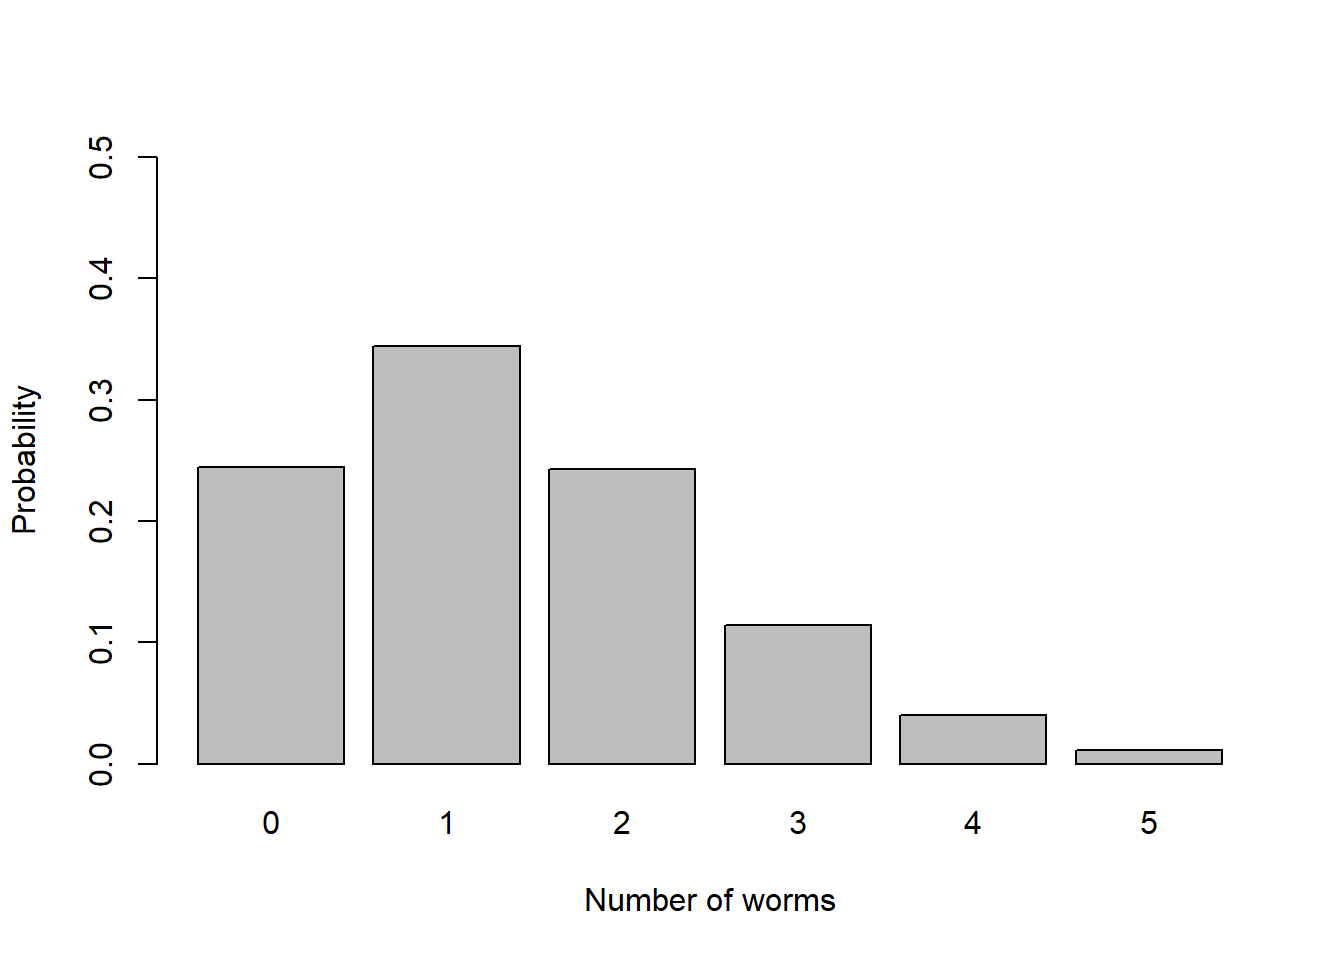
\includegraphics[width=0.5\linewidth,height=0.5\textheight]{_main_files/figure-latex/unnamed-chunk-49-1} \end{center}

Now change the plot so that the cumulative probabilities are plotted. You will need to change the code to use \texttt{ppois()} instead of \texttt{dpois()}, as well as the y-axis limits (\texttt{ylim}).

\begin{Shaded}
\begin{Highlighting}[]
\CommentTok{\# create new columns in worm\_df for the probabilities}
\NormalTok{worm\_df}\SpecialCharTok{$}\NormalTok{prob }\OtherTok{\textless{}{-}} \FunctionTok{dpois}\NormalTok{(worm\_df}\SpecialCharTok{$}\NormalTok{num\_worms, lambda)}
\NormalTok{worm\_df}\SpecialCharTok{$}\NormalTok{cumul\_prob }\OtherTok{\textless{}{-}} \FunctionTok{cumsum}\NormalTok{(worm\_df}\SpecialCharTok{$}\NormalTok{prob)}
\end{Highlighting}
\end{Shaded}

\begin{Shaded}
\begin{Highlighting}[]
\CommentTok{\# Make Table 2.1. Use packageName::function() instead of loading with library()}
\NormalTok{knitr}\SpecialCharTok{::}\FunctionTok{kable}\NormalTok{(worm\_df, }\AttributeTok{digits=}\DecValTok{5}\NormalTok{,}
             \AttributeTok{caption =} \StringTok{\textquotesingle{}Worm cast observations and expected probabilities.\textquotesingle{}}\NormalTok{) }
\end{Highlighting}
\end{Shaded}

\begin{table}

\caption{\label{tab:worm-table}Worm cast observations and expected probabilities.}
\centering
\begin{tabular}[t]{r|r|r|r}
\hline
num\_worms & num\_quadrats & prob & cumul\_prob\\
\hline
0 & 35 & 0.24414 & 0.24414\\
\hline
1 & 28 & 0.34424 & 0.58839\\
\hline
2 & 15 & 0.24269 & 0.83108\\
\hline
3 & 10 & 0.11406 & 0.94514\\
\hline
4 & 7 & 0.04021 & 0.98535\\
\hline
5 & 5 & 0.01134 & 0.99669\\
\hline
6 & 0 & 0.00266 & 0.99935\\
\hline
\end{tabular}
\end{table}

\emph{Q64. Format the probabilities in the table to 3 significant figures.}

If individual probability values (not cumulative probability) are multiplied by the total number of quadrats thrown (100), we generate the expected frequency distribution for comparison with the observed results above.

\emph{Q65. Write the appropriate code to add a column(called \texttt{num\_quadrats\_expected}) to `worm\_df' that is the expected number of quadrats (given that 100 quadrats was the total thrown).}

This expected number is the number of quadrats that you would expect to contain 0,1,\ldots,5 worms, given that the mean density of worms is 1.41. The number of worms per quadrat is a discrete variable, yet you can have non-integer `expectations' (i.e.~means).

\emph{Q66. Add another column that is the difference in the Expected number of quadrats and \texttt{num\_quadrats\_expected}.}

\emph{Q67. Produce a bar graph of this difference.}

\begin{center}\rule{0.5\linewidth}{0.5pt}\end{center}

\hypertarget{the-poisson-approximation-of-the-binomial-model}{%
\section{The Poisson approximation of the binomial model}\label{the-poisson-approximation-of-the-binomial-model}}

Where the number of trials is large and the probability of success is small, the Poisson distribution can be used as an approximation of the binomial distribution. Under these circumstances you can calculate the mean of a variable that has a binomial distribution (number of trials x probability of success; \(n*p\)) and use that as an estimate of \(\lambda\) in the Poisson model. The reason why you may wish to do this is because the Poisson model is much easier to use than the binomial model when \(n\) is large.

There are several rules of thumb that apply here. Some say that when \(p<0.1\), the Poisson approximation may be preferable to the binomial, other texts state that \(n\) should be \textgreater{} 50 and \(p<0.05\) (so \(n * p = \lambda = 2.5\)) whilst others state \(n>100\) and \(n*p<10\). The point is that as \(n\) increases and \(p\) decreases, the approximation gets better.

There are an infinite number of ways of multiplying two numbers together to get 5. Call our numbers \(p\) and \(k\). For example, when \(p=0.5\), \(n=10\) OR when \(p=0.05\), \(n=100\), \(n*p=5\). We can use this to illustrate the Poisson approximation of the binomial distribution.

\begin{Shaded}
\begin{Highlighting}[]
\CommentTok{\# generate dataframe with probability for 0:16 \textquotesingle{}successes\textquotesingle{} from different }
\CommentTok{\# distributions but where mean is 5.}
\CommentTok{\# note that in y \textasciitilde{} Binom(10,0.5), probability of \textgreater{}10 successes is zero.}
\CommentTok{\# We\textquotesingle{}re going to leverage the power of the tidyverse here}
\FunctionTok{library}\NormalTok{(tidyverse)}
\NormalTok{y\_seq }\OtherTok{\textless{}{-}} \DecValTok{0}\SpecialCharTok{:}\DecValTok{16}
\NormalTok{binom\_df }\OtherTok{\textless{}{-}} \FunctionTok{tibble}\NormalTok{(}\AttributeTok{y=}\FunctionTok{rep}\NormalTok{(y\_seq, }\AttributeTok{times=}\DecValTok{3}\NormalTok{), }\CommentTok{\# ?rep}
                   \AttributeTok{n=}\FunctionTok{rep}\NormalTok{(}\FunctionTok{c}\NormalTok{(}\DecValTok{10}\NormalTok{, }\DecValTok{20}\NormalTok{, }\DecValTok{100}\NormalTok{), }\AttributeTok{each=}\FunctionTok{length}\NormalTok{(y\_seq)),}
                   \AttributeTok{p=}\FunctionTok{rep}\NormalTok{(}\FunctionTok{c}\NormalTok{(}\FloatTok{0.5}\NormalTok{, }\FloatTok{0.25}\NormalTok{, }\FloatTok{0.05}\NormalTok{), }\AttributeTok{each=}\FunctionTok{length}\NormalTok{(y\_seq))) }\SpecialCharTok{|\textgreater{}}
    \FunctionTok{mutate}\NormalTok{(}\AttributeTok{mean=}\NormalTok{n}\SpecialCharTok{*}\NormalTok{p,}
           \AttributeTok{prob=}\FunctionTok{dbinom}\NormalTok{(y\_seq, n, p),}
           \AttributeTok{label=}\FunctionTok{paste0}\NormalTok{(}\StringTok{"y \textasciitilde{} Binom("}\NormalTok{, n, }\StringTok{", "}\NormalTok{, p, }\StringTok{")"}\NormalTok{))}
\NormalTok{pois\_df }\OtherTok{\textless{}{-}} \FunctionTok{tibble}\NormalTok{(}\AttributeTok{y=}\NormalTok{y\_seq,}
                  \AttributeTok{n=}\ConstantTok{NA}\NormalTok{, }
                  \AttributeTok{p=}\ConstantTok{NA}\NormalTok{,}
                  \AttributeTok{mean=}\DecValTok{5}\NormalTok{) }\SpecialCharTok{|\textgreater{}}
    \FunctionTok{mutate}\NormalTok{(}\AttributeTok{prob=}\FunctionTok{dpois}\NormalTok{(y\_seq, mean),}
           \AttributeTok{label=}\FunctionTok{paste0}\NormalTok{(}\StringTok{"y \textasciitilde{} Pois("}\NormalTok{, mean, }\StringTok{")"}\NormalTok{))}
\NormalTok{PDF\_df }\OtherTok{\textless{}{-}} \FunctionTok{bind\_rows}\NormalTok{(binom\_df, pois\_df) }\SpecialCharTok{|\textgreater{}}
  \FunctionTok{mutate}\NormalTok{(}\AttributeTok{label=}\FunctionTok{factor}\NormalTok{(label, }\AttributeTok{levels=}\FunctionTok{unique}\NormalTok{(label)))}
\end{Highlighting}
\end{Shaded}

\begin{Shaded}
\begin{Highlighting}[]
\FunctionTok{head}\NormalTok{(binom\_df, }\DecValTok{2}\NormalTok{)}
\end{Highlighting}
\end{Shaded}

\begin{verbatim}
## # A tibble: 2 x 6
##       y     n     p  mean     prob label             
##   <int> <dbl> <dbl> <dbl>    <dbl> <chr>             
## 1     0    10   0.5     5 0.000977 y ~ Binom(10, 0.5)
## 2     1    10   0.5     5 0.00977  y ~ Binom(10, 0.5)
\end{verbatim}

\begin{Shaded}
\begin{Highlighting}[]
\FunctionTok{head}\NormalTok{(pois\_df, }\DecValTok{2}\NormalTok{)}
\end{Highlighting}
\end{Shaded}

\begin{verbatim}
## # A tibble: 2 x 6
##       y n     p      mean    prob label      
##   <int> <lgl> <lgl> <dbl>   <dbl> <chr>      
## 1     0 NA    NA        5 0.00674 y ~ Pois(5)
## 2     1 NA    NA        5 0.0337  y ~ Pois(5)
\end{verbatim}

\begin{Shaded}
\begin{Highlighting}[]
\FunctionTok{ggplot}\NormalTok{(PDF\_df, }\FunctionTok{aes}\NormalTok{(y, prob, }\AttributeTok{fill=}\NormalTok{label)) }\SpecialCharTok{+}  \CommentTok{\# ggplot(data, aes(xVar, yVar))}
  \FunctionTok{geom\_bar}\NormalTok{(}\AttributeTok{stat=}\StringTok{"identity"}\NormalTok{, }\AttributeTok{position=}\StringTok{"dodge"}\NormalTok{, }\AttributeTok{colour=}\StringTok{"grey30"}\NormalTok{) }\SpecialCharTok{+}  \CommentTok{\# ?geom\_bar}
  \FunctionTok{scale\_fill\_brewer}\NormalTok{(}\StringTok{"Distribution"}\NormalTok{, }\AttributeTok{palette=}\StringTok{"Purples"}\NormalTok{) }\SpecialCharTok{+} \CommentTok{\# from colorbrewer2.org}
  \FunctionTok{labs}\NormalTok{(}\AttributeTok{x=}\StringTok{"Number of successes with mean = 5"}\NormalTok{, }\AttributeTok{y=}\StringTok{"Probability"}\NormalTok{) }\SpecialCharTok{+}
  \FunctionTok{theme\_classic}\NormalTok{() }\SpecialCharTok{+} \FunctionTok{theme}\NormalTok{(}\AttributeTok{legend.position=}\FunctionTok{c}\NormalTok{(}\FloatTok{0.85}\NormalTok{, }\FloatTok{0.85}\NormalTok{))}
\end{Highlighting}
\end{Shaded}

\begin{figure}

{\centering 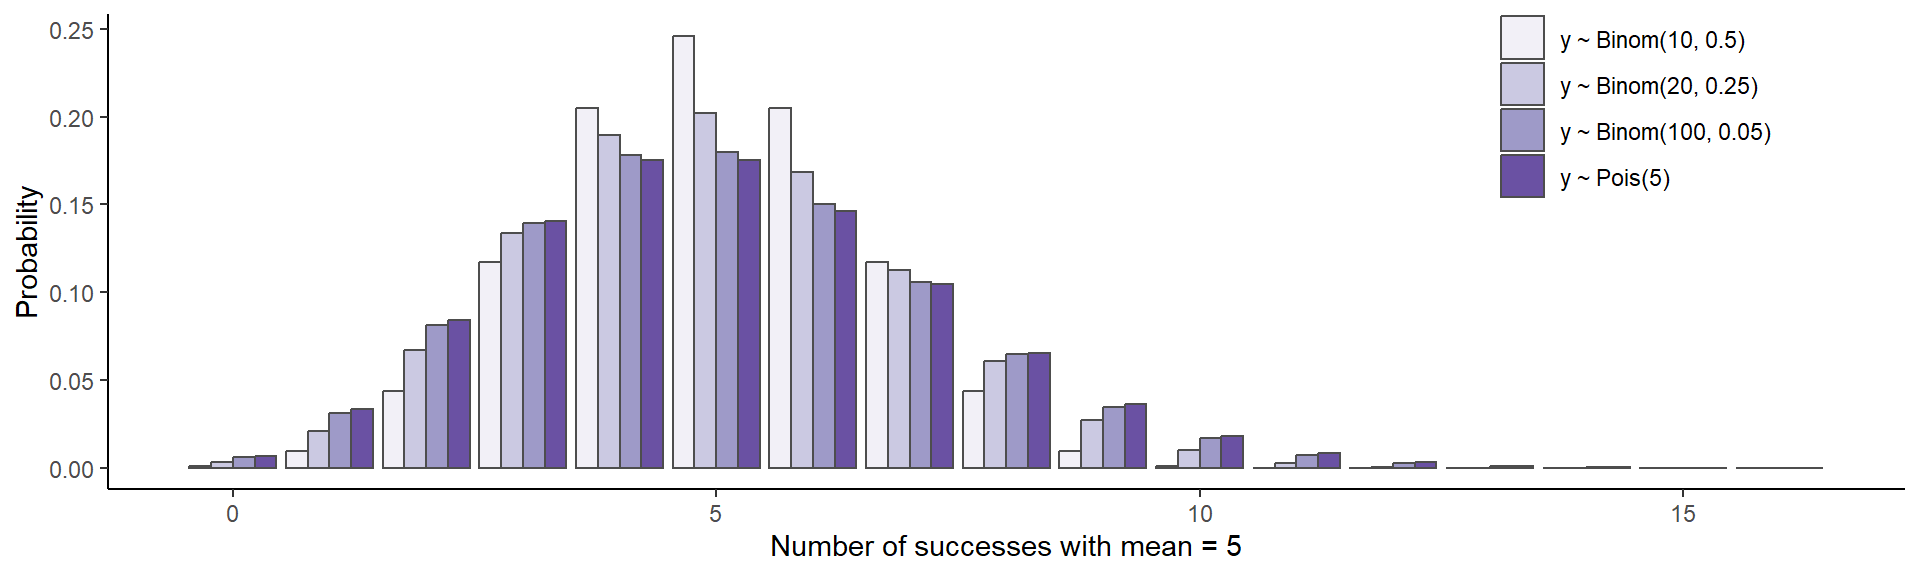
\includegraphics[width=1\linewidth,height=1\textheight]{_main_files/figure-latex/binom-pois-approx-1} 

}

\caption{Binomial and Poisson distributions converge with larger numbers of events.}\label{fig:binom-pois-approx}
\end{figure}

\emph{Q68. What is the modal value in these distributions?}

Generate some random numbers from the distributions in Fig \ref{fig:binom-pois-approx} and calculate their mean and variance. Here is \(y \sim Pois(5)\):

\begin{Shaded}
\begin{Highlighting}[]
\NormalTok{y }\OtherTok{\textless{}{-}} \FunctionTok{rpois}\NormalTok{(}\DecValTok{10000}\NormalTok{, }\DecValTok{5}\NormalTok{)}
\FunctionTok{paste0}\NormalTok{(}\StringTok{"Mean: "}\NormalTok{, }\FunctionTok{signif}\NormalTok{(}\FunctionTok{mean}\NormalTok{(y), }\DecValTok{3}\NormalTok{), }\StringTok{", variance: "}\NormalTok{, }\FunctionTok{signif}\NormalTok{(}\FunctionTok{var}\NormalTok{(y), }\DecValTok{3}\NormalTok{))}
\end{Highlighting}
\end{Shaded}

\begin{verbatim}
## [1] "Mean: 4.97, variance: 5.02"
\end{verbatim}

\emph{Q69. What do you notice about the mean and variance in the Poisson model?}

\emph{Q70. What do you notice about the mean and variance in the binomial models as} \(n\) \emph{increases and} \(p\) \emph{decreases? When is it more similar to the Poisson? Is this what you expected?}

\begin{center}\rule{0.5\linewidth}{0.5pt}\end{center}

\hypertarget{conclusions-1}{%
\section{Conclusions}\label{conclusions-1}}

The binomial distribution is a discrete probability distribution that models situations where the outcome of an observation or experiment is binary (i.e., two possibilities) or can be coded as such. The binomial model enables us to predict the probability of making our observation or series of independent observations for any given probability of a success (\(p\)). This enables us to quantify how likely our observation is to have occurred, by chance. If the chance of our observation is very low, we can challenge the hypothesis with regard the probability of success (\(p\)) and suggest a different value.

The Poisson distribution is another discrete probability distribution that is used to predict the chance occurrence of observations that are rare, independent and randomly distributed with mean = variance = \(\lambda\). The Poisson distribution can be used as an approximation of the binomial distribution where the number of trials (\(n\)) is large and the probability of success (\(p\)) is small. This approximation is useful as, unlike the Poisson distribution, the binomial calculation requires the handling of massive numbers (from large factorials).

\hypertarget{normal}{%
\chapter{Normal distribution}\label{normal}}

Statistical inference is the process by which we infer from a sample statistic to the population. We need to infer from samples to populations because it is usually impossible to measure the entire populations. We call this this estimating population parameters from samples.

In order to infer from samples to populations we need to understand/predict how the statistics we generate from our samples `behave'. To do this we use theoretical distributions.

\emph{Q71. Which two theoretical distributions have we already covered in this course?}

The normal (a.k.a., Gaussian) distribution is another theoretical distribution and is central to inferential statistics. If your data (or, more accuarately, statistics derived from you data) are reasonably approximated by the normal distribution then you will be able to use a wide range of techniques to deal with it.

In this practical we will be examining the normal distribution, calculating Z scores both manually and in R, and interpreting those Z scores. We'll also use our knowledge of the normal distribution's behaviour to produce confidence intervals and assess whether data are reasonably assummed to be normally distributed, transforming the data where they are not. We'll apply the CLT and evaluate how well other distributions are approximated by the normal distribution.

\begin{center}\rule{0.5\linewidth}{0.5pt}\end{center}

\hypertarget{using-the-normal-probability-distributions}{%
\section{Using the normal probability distributions}\label{using-the-normal-probability-distributions}}

The length, in cm, of a catch of herring was measured. Five hundred individuals were studied. We will consider this group to be the entire population of interest. The population parameters are: mean length 37.6 cm, standard deviation 1.20 cm.

\emph{Q72. What are the theoretical limits of the normal distribution?}

\emph{Q73. Do you think normality a fair assumption for these data?}

\emph{Q74. Assume length of herring is approximately normally distributed and write down the model which describes the fish length distribution in the standard notation.}

When we have population parameters such as we have here, we can calculate Z scores for individuals (or groups of individuals) from that population and calculate how unusual they are. For the moment, we are interested in determining what proportion of fish from this population expected to be \textless38cm.

\emph{Q75. Sketch a normal distribution, showing mean of 37.6cm, note the sd on your sketch and sketch on the location of a fish at 38 cm.}

\emph{Q76. Mark-out the bit of the sketch which the question asks you about}

\emph{Q77. Mark out the bit of the sketch that our manually determined Z scores relate to.}

\emph{Q78. Calculate the Z score for a fish of 38cm. How unusual is such an observation? What proportion of fish will be \textless38 cm, what proportion of fish \textgreater38 cm?.}

\hypertarget{using-r-to-calculate-areas-under-the-normal-curve}{%
\subsection{Using R to calculate areas under the normal curve}\label{using-r-to-calculate-areas-under-the-normal-curve}}

To solve this problem using R we use cumulative probability. Observations at the extreme low end are extremely unlikely, but the probability of observing data increases and reaches a maximum at the mean, after which it declines again. The normal distribution is symmetrical.

\emph{Q79. What shape is the cumulative probability curve of a normally distributed variable?}

You can ask R to determine the probabilities of an eventuality occurring within a normal distribution. For example, you could ask what the probability is of observing a 38 cm or more fish, when the mean is 37.6 cm and the standard deviation is 1.20 cm. You need to specify the model, and the problem. Use \texttt{?dnorm} and look at your options.

\begin{Shaded}
\begin{Highlighting}[]
\CommentTok{\# cumulative probability: which bit of the curve does this relate to?}
\FunctionTok{pnorm}\NormalTok{(}\AttributeTok{q =} \DecValTok{38}\NormalTok{, }\AttributeTok{mean =} \FloatTok{37.6}\NormalTok{, }\AttributeTok{sd =} \FloatTok{1.2}\NormalTok{) }
\end{Highlighting}
\end{Shaded}

\begin{figure}

{\centering 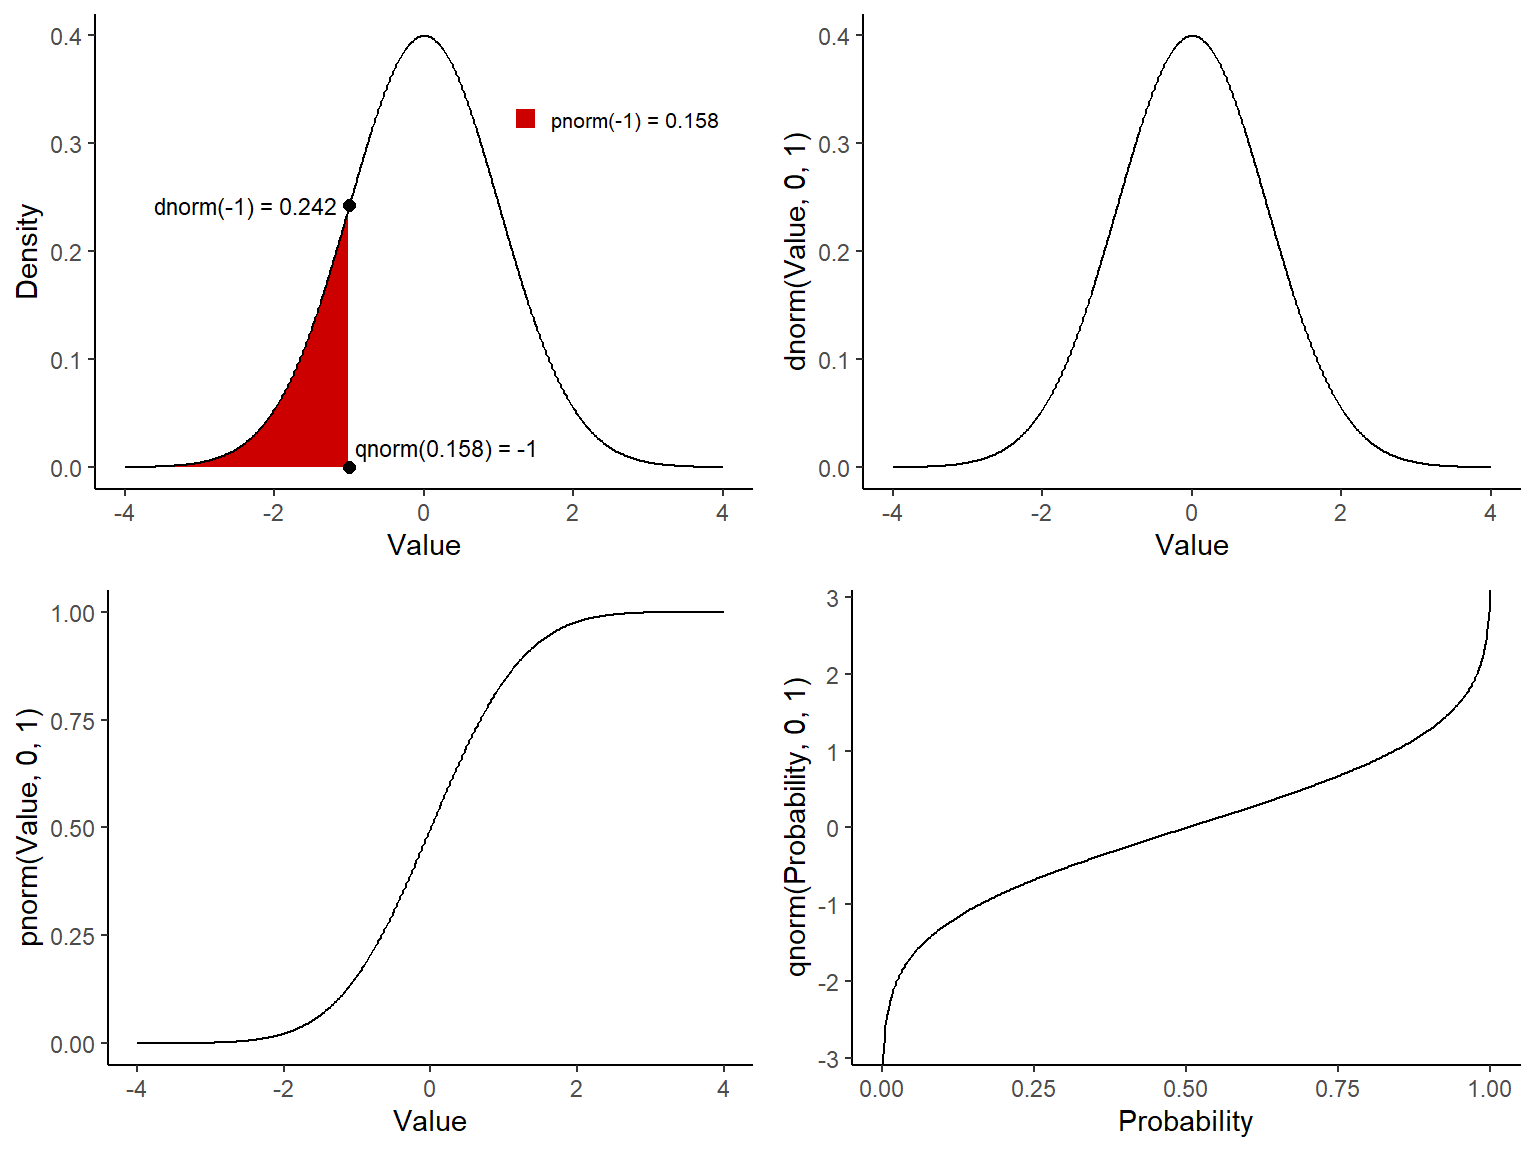
\includegraphics[width=0.8\linewidth,height=0.8\textheight]{_main_files/figure-latex/dpq-examp-1} 

}

\caption{Functions for distributions in R illustrated with a standard normal.}\label{fig:dpq-examp}
\end{figure}

We can plot any normal distribution we like. Play with the values for \texttt{mu} and \texttt{sigma} below, adjusting the values for \texttt{from} and \texttt{to} as needed to see the distribution.

\begin{Shaded}
\begin{Highlighting}[]
\NormalTok{mu }\OtherTok{\textless{}{-}} \FloatTok{37.6}  \CommentTok{\# population mean}
\NormalTok{sigma }\OtherTok{\textless{}{-}} \FloatTok{1.2}  \CommentTok{\# population sd}
\FunctionTok{curve}\NormalTok{(}\FunctionTok{dnorm}\NormalTok{(x, }\AttributeTok{mean =}\NormalTok{ mu, }\AttributeTok{sd =}\NormalTok{ sigma), }\AttributeTok{from =} \DecValTok{30}\NormalTok{, }\AttributeTok{to =} \DecValTok{45}\NormalTok{,}
      \AttributeTok{main =} \StringTok{"Normal density"}\NormalTok{, }\AttributeTok{ylab =} \StringTok{"Density"}\NormalTok{, }\AttributeTok{xlab =} \StringTok{"Fish length, cm"}\NormalTok{)}
\end{Highlighting}
\end{Shaded}

I can define a population like this \(y \sim Norm(37.6, 1.2)\) and ask questions about \(P(y_i \leq a)\). E.g., what is the probability that a random fish drawn from this population is \textless38 cm (\(P(y_i < 38)\)). The answer to that is 0.6306 or approximately 63\% (2 sf).

\emph{Q80. How does your hand calculation compare? Is there a discrepancy? If so, why?}

\begin{center}\rule{0.5\linewidth}{0.5pt}\end{center}

\hypertarget{normal-model-adequacy}{%
\section{Normal model adequacy}\label{normal-model-adequacy}}

A separate fish population (long-eared wrasse) is described as \(y \sim Norm(5.14 cm, 25 cm)\).

\emph{Q81. What is the mean length and standard deviation of long-eared wrasse?}

\emph{Q82. Calculate the proportion of fish that are less than zero cm in length.}

\emph{Q84. What do your results indicate about the adequacy of the normal model to describe the length distribution of long-eared wrasse?}

\emph{Q85. Recalculate your answers with 1/10\textsuperscript{th} the standard deviation:} \(y \sim Norm(5.14, 2.5)\)\emph{.}

\begin{center}\rule{0.5\linewidth}{0.5pt}\end{center}

\hypertarget{calculating-quantiles-in-the-normal-distribution}{%
\section{Calculating quantiles in the normal distribution}\label{calculating-quantiles-in-the-normal-distribution}}

A quantile is one of a series of values that divides a frequency distribution (i.e.~a set of numbers) into equally represented groups (i.e., the same number of observations per group). For example, there are three values (Q1, Q2, Q3) that split a normal distribution into four groups (negative infinity to Q1, Q1 to Q2 (median), Q2 to Q3, and Q3 to positive infinity). Q3 - Q2 is the middle 50\% of the data: the interquartile range.

There are 99 quantiles, called percentiles, that split your data into 100 groups. The 2.5 percentile is the value that splits your data into two groups corresponding to 2.5\% along the distribution (from negative infinity for the normal distribution). Just as we can ask what proportion of a distribution is above or below a set value, we can also ask between what values will a given percentage of my data lie (e.g.~what values correspond to the middle 95\%?).

To solve this problem using R we use the cumulative probability function \texttt{qnorm()}.

\begin{Shaded}
\begin{Highlighting}[]
\FunctionTok{qnorm}\NormalTok{(}\AttributeTok{p =} \FloatTok{0.975}\NormalTok{, }\AttributeTok{mean =} \FloatTok{37.6}\NormalTok{, }\AttributeTok{sd =} \FloatTok{1.2}\NormalTok{) }\CommentTok{\# p is the cumulative probability }
\end{Highlighting}
\end{Shaded}

\begin{verbatim}
## [1] 39.95196
\end{verbatim}

\begin{Shaded}
\begin{Highlighting}[]
\NormalTok{probs }\OtherTok{\textless{}{-}} \FunctionTok{seq}\NormalTok{(}\AttributeTok{from =} \FloatTok{0.1}\NormalTok{, }\AttributeTok{to =} \FloatTok{0.9}\NormalTok{, }\AttributeTok{by =} \FloatTok{0.2}\NormalTok{) }\CommentTok{\# vectorize for \textgreater{}1 probability}
\FunctionTok{qnorm}\NormalTok{(}\AttributeTok{p =}\NormalTok{ probs, }\AttributeTok{mean =} \FloatTok{37.6}\NormalTok{, }\AttributeTok{sd =} \FloatTok{1.2}\NormalTok{) }
\end{Highlighting}
\end{Shaded}

\begin{verbatim}
## [1] 36.06214 36.97072 37.60000 38.22928 39.13786
\end{verbatim}

\begin{Shaded}
\begin{Highlighting}[]
\NormalTok{probs\_95 }\OtherTok{\textless{}{-}} \FunctionTok{c}\NormalTok{(}\FloatTok{0.025}\NormalTok{, }\FloatTok{0.975}\NormalTok{) }\CommentTok{\# middle 95\% (2.5\% on either side)}
\FunctionTok{qnorm}\NormalTok{(}\AttributeTok{p =}\NormalTok{ probs\_95, }\AttributeTok{mean =} \FloatTok{37.6}\NormalTok{, }\AttributeTok{sd =} \FloatTok{1.2}\NormalTok{) }\CommentTok{\# round as appropriate}
\end{Highlighting}
\end{Shaded}

\begin{verbatim}
## [1] 35.24804 39.95196
\end{verbatim}

These values (\texttt{probs\_95\ =\ c(0.025,\ 0.975)}) identify proportions of the cumulative curve. That is, they identify the bottom 2.5\% and the bottom 97.5\% of the curve. Values between these two parameters will constitute the central 95\% of your data.

For the next question, return to the herring data where the population was \(y \sim Norm(37.6, 1.44)\).

\emph{Q86. Find the values that capture the middle 95 and 90\% of the herring data.}

We quote our mean and interval like this: ``The mean fish length and 95\% interval was 37.6 cm (35.2 cm, 40.0 cm)''. Remember to use to same degree of precision (significant figures) for confidence intervals as was used to gather the data (or as specified in the question, defaulting to three).

\emph{Q87. What value would you expect to correspond to 0.5 (i.e., what value would be found half-way along your distribution)?}

\emph{Q88. Check your answer above using \texttt{qnorm()}}

You can easily visualise this distribution in R:

\begin{Shaded}
\begin{Highlighting}[]
\CommentTok{\# your population is defined thus: y \textasciitilde{} Norm(mean=100, variance=225) }
\NormalTok{mu }\OtherTok{\textless{}{-}} \DecValTok{100}
\NormalTok{sigma }\OtherTok{\textless{}{-}} \DecValTok{15}
\CommentTok{\# lower boundary and upper boundary of the region of interest}
\NormalTok{lb }\OtherTok{\textless{}{-}} \DecValTok{80}
\NormalTok{ub }\OtherTok{\textless{}{-}} \DecValTok{140} 

\NormalTok{x }\OtherTok{\textless{}{-}} \FunctionTok{seq}\NormalTok{(}\SpecialCharTok{{-}}\DecValTok{4}\NormalTok{, }\DecValTok{4}\NormalTok{, }\AttributeTok{length.out =} \DecValTok{100}\NormalTok{) }\SpecialCharTok{*}\NormalTok{ sigma }\SpecialCharTok{+}\NormalTok{ mu}
\NormalTok{hx }\OtherTok{\textless{}{-}} \FunctionTok{dnorm}\NormalTok{(x, mu, sigma)}
\FunctionTok{plot}\NormalTok{(x, hx,}
  \AttributeTok{type =} \StringTok{"n"}\NormalTok{, }\AttributeTok{xlab =} \StringTok{"IQ Values"}\NormalTok{, }\AttributeTok{ylab =} \StringTok{""}\NormalTok{,}
  \AttributeTok{main =} \StringTok{"Normal Distribution"}\NormalTok{, }\AttributeTok{axes =} \ConstantTok{FALSE}
\NormalTok{)}
\NormalTok{i }\OtherTok{\textless{}{-}}\NormalTok{ x }\SpecialCharTok{\textgreater{}=}\NormalTok{ lb }\SpecialCharTok{\&}\NormalTok{ x }\SpecialCharTok{\textless{}=}\NormalTok{ ub}
\FunctionTok{lines}\NormalTok{(x, hx)}
\FunctionTok{polygon}\NormalTok{(}\FunctionTok{c}\NormalTok{(lb, x[i], ub), }\FunctionTok{c}\NormalTok{(}\DecValTok{0}\NormalTok{, hx[i], }\DecValTok{0}\NormalTok{), }\AttributeTok{col =} \StringTok{"red"}\NormalTok{) }\CommentTok{\# create 100 polygons}
\NormalTok{area }\OtherTok{\textless{}{-}} \FunctionTok{pnorm}\NormalTok{(ub, mu, sigma) }\SpecialCharTok{{-}} \FunctionTok{pnorm}\NormalTok{(lb, mu, sigma)}
\NormalTok{result }\OtherTok{\textless{}{-}} \FunctionTok{paste}\NormalTok{(}
  \StringTok{"P("}\NormalTok{, lb, }\StringTok{"\textless{} IQ \textless{}"}\NormalTok{, ub, }\StringTok{") ="}\NormalTok{,}
  \FunctionTok{signif}\NormalTok{(area, }\AttributeTok{digits =} \DecValTok{3}\NormalTok{)}
\NormalTok{)}
\FunctionTok{mtext}\NormalTok{(result, }\DecValTok{3}\NormalTok{)}
\FunctionTok{axis}\NormalTok{(}\DecValTok{1}\NormalTok{, }\AttributeTok{at =} \FunctionTok{seq}\NormalTok{(}\FunctionTok{floor}\NormalTok{(mu }\SpecialCharTok{{-}} \DecValTok{4}\SpecialCharTok{*}\NormalTok{sigma), }\FunctionTok{floor}\NormalTok{(mu }\SpecialCharTok{+} \DecValTok{4}\SpecialCharTok{*}\NormalTok{sigma), sigma), }\AttributeTok{pos =} \DecValTok{0}\NormalTok{)}
\end{Highlighting}
\end{Shaded}

\begin{figure}

{\centering 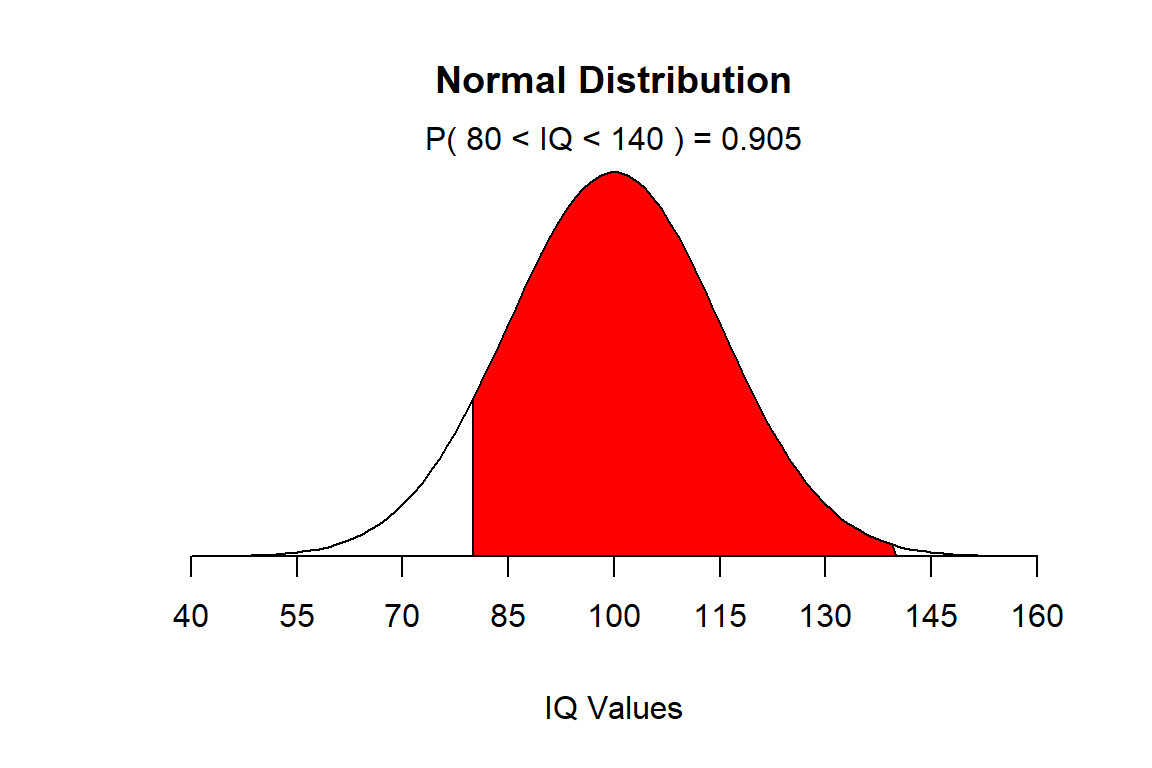
\includegraphics[width=0.6\linewidth,height=0.6\textheight]{_main_files/figure-latex/iq-examp-1} 

}

\caption{The normal distribution illustrating probability of a random individual from your population having an IQ between 80 and 140.}\label{fig:iq-examp}
\end{figure}

\emph{Q89. Change the parameters in the above to your herring data where the population was distributed} \(y \sim Norm(37.6, 1.44)\) \emph{and check that the values you generated for the 95\% interval correspond when plugged into \texttt{lb} and \texttt{ub} in the code.}

\emph{Q90. What is the difference between} \(< x\) \emph{and} \(\leq x\) \emph{when applied to continuous data?}

\emph{Q91. Does this also apply to discontinuous data?}

Think about how intervals change when the population standard deviation changes.

\emph{Q92. With everything else equal, try doubling, quadrupling, and halving the standard deviation on the herring data then re-running the same code.}

\emph{Q93. What effect does this have on your interval?}

\begin{center}\rule{0.5\linewidth}{0.5pt}\end{center}

\hypertarget{testing-for-normality}{%
\section{Testing for normality}\label{testing-for-normality}}

As we note in the lectures, many statistical tests require that data are reasonably approximated by a normal distribution and have homogeneous variance. R can be used to formally test the assumption that data are normally distributed, though you should have some idea of whether this is likely through consideration of the data source. This applies particularly where you have a small sample size and, consequently, evaluating the distribution is challenging.

The data you collect will be part of a population. The normality check assesses the viability of the assumption that the data you collected were drawn from a population that was normally distributed. You should note that populations are, in practice, \emph{never} actually normally distributed. Your test is to assess how \emph{reasonable} the assumption of normality is.

\begin{Shaded}
\begin{Highlighting}[]
\FunctionTok{library}\NormalTok{(readxl) }
\NormalTok{MS }\OtherTok{\textless{}{-}} \FunctionTok{read\_xlsx}\NormalTok{(}\StringTok{"data/practical\_3\_4.xlsx"}\NormalTok{, }\AttributeTok{sheet =} \StringTok{"Mood shrimp"}\NormalTok{)}
\CommentTok{\# check the data using head(), str() etc.}
\end{Highlighting}
\end{Shaded}

\begin{Shaded}
\begin{Highlighting}[]
\FunctionTok{par}\NormalTok{(}\AttributeTok{mfrow =} \FunctionTok{c}\NormalTok{(}\DecValTok{1}\NormalTok{, }\DecValTok{2}\NormalTok{))}
\FunctionTok{qqnorm}\NormalTok{(MS}\SpecialCharTok{$}\NormalTok{Shrimp1)}
\FunctionTok{qqline}\NormalTok{(MS}\SpecialCharTok{$}\NormalTok{Shrimp1, }\AttributeTok{col =} \DecValTok{2}\NormalTok{) }\CommentTok{\# the data fall near the line}
\FunctionTok{qqnorm}\NormalTok{(MS}\SpecialCharTok{$}\NormalTok{Shrimp2)}
\FunctionTok{qqline}\NormalTok{(MS}\SpecialCharTok{$}\NormalTok{Shrimp1, }\AttributeTok{col =} \DecValTok{2}\NormalTok{) }\CommentTok{\# the data deviate widely from the line}
\end{Highlighting}
\end{Shaded}

\begin{figure}

{\centering 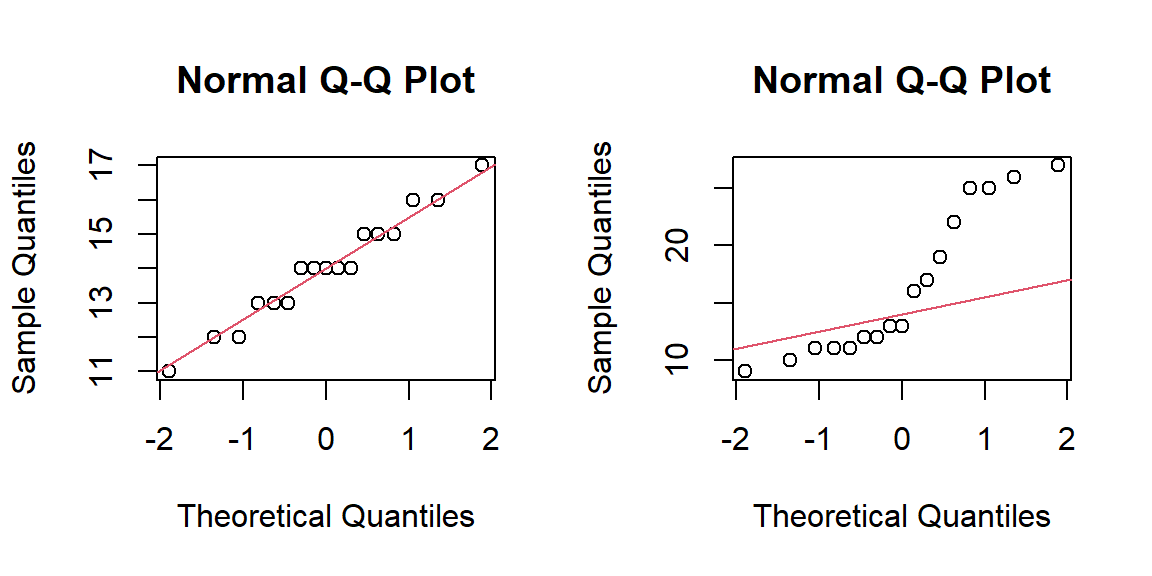
\includegraphics[width=0.5\linewidth,height=0.5\textheight]{_main_files/figure-latex/qq-examp-1} 

}

\caption{Normal (QQ) plots. The left indicates that the normality assumption might be reasonable, not so on the right.}\label{fig:qq-examp}
\end{figure}

The axes on the probability plots have been rescaled so that, if your data are perfectly normal, the data points would fall on a straight line (the red line on the graphs generated by \texttt{qqline()}). Any deviation from the red straight line in your data indicates a lack of normality. What we need to assess is how serious any deviation is and whether it is sufficient to indicate that the assumption of normality is not `reasonable'. This is a subjective decision, and two different statisticians may tell you different answers about the same data.

As your sample size decreases, it will be increasingly difficult to see if your data are reasonably approximated by a normal distribution. There are many formal statistical methods for assessing normality, but as we already know it is impossible for your data to have been drawn from a population that is normal and this means such tests are largely redundant. You must assess the assumptions of your model (e.g.~the general linear model, which includes ANOVA and linear regression), but you should be aware that all data fails the assumptions. However, this doesn't mean the outputs from such models aren't useful - provided the assumptions are `reasonably' well met. There is no hard rule as to what constitutes `reasonable'!

\emph{Q94. Make histograms of both \texttt{Shrimp1} and \texttt{Shrimp2}. Comment on their apparent distributions.}

\begin{center}\rule{0.5\linewidth}{0.5pt}\end{center}

\hypertarget{transformations}{%
\section{Data transformations}\label{transformations}}

The assumption that our sample data are drawn from a normally distributed population is central to the use of many important inferential statistical techniques. However, frequently it is \emph{not} reasonable to assume that data are likely to be normally distributed and they `fail' normality tests (e.g.~clearly do not fall on the red \texttt{qqline()}).

Non-normality often occurs because our measurements are near a logical zero. For example, chemical concentrations (e.g., of zinc in sediments) is limited by zero; you cannot have negative zinc concentrations. Similarly, you cannot have negative lengths, time, mass, etc. Where data is collected `near' a logical zero they are often not normally distributed, since the normal distribution predicts a negative-value `tail' which is impossible.

There are several simple mathematical transformation options that you can use in an attempt to convert your data to something that is reasonably approximated by a normal distribution even if it is not well approximated in the original measurement units.

Here we will consider three common transformations. These are the log (base 10 or natural), the square-root, and the arcsine transformation. These transformations often have the additional benefit of correcting unequal variances (see Practical \ref{glm}) in addition to non-normality so they are very useful. These three are often used in distinct circumstances.

\begin{itemize}
\tightlist
\item
  Log (\texttt{log()}): When the distribution is skewed right. Often `cures' heteroscedasticity.\\
\item
  Square-root (\texttt{sqrt()}): When the measurements are areas (e.g., leaf areas). Often used to `down-weight' common species (e.g., Practical \ref{multivariate}), which is unrelated to model assumptions.\\
\item
  Arcsine (\texttt{asin()}): When the measurements are percentages or proportions. Tends to stretch out the tails (e.g., near 0 or 1 for proportions) and squash the middle (e.g., near 0.5).
\end{itemize}

Identifying the correct transformation can be led by an underlying comprehension of the nature of the data. However, this often doesn't work so expect some trial and error.

\begin{Shaded}
\begin{Highlighting}[]
\NormalTok{a }\OtherTok{\textless{}{-}} \FunctionTok{seq}\NormalTok{(}\FloatTok{0.01}\NormalTok{, }\DecValTok{100}\NormalTok{, }\AttributeTok{length.out=}\DecValTok{100}\NormalTok{)}
\NormalTok{b }\OtherTok{\textless{}{-}} \FunctionTok{seq}\NormalTok{(}\FloatTok{0.01}\NormalTok{, }\FloatTok{0.99}\NormalTok{, }\AttributeTok{length.out=}\DecValTok{100}\NormalTok{)}

\FunctionTok{par}\NormalTok{(}\AttributeTok{mfrow=}\FunctionTok{c}\NormalTok{(}\DecValTok{2}\NormalTok{,}\DecValTok{3}\NormalTok{), }\AttributeTok{mar=}\FunctionTok{c}\NormalTok{(}\DecValTok{4}\NormalTok{,}\DecValTok{4}\NormalTok{,}\DecValTok{1}\NormalTok{,}\DecValTok{1}\NormalTok{))}
\FunctionTok{plot}\NormalTok{(a, a}\SpecialCharTok{\^{}}\FloatTok{0.5}\NormalTok{, }\AttributeTok{type=}\StringTok{"l"}\NormalTok{)}
\FunctionTok{plot}\NormalTok{(a, }\FunctionTok{log}\NormalTok{(a), }\AttributeTok{type=}\StringTok{"l"}\NormalTok{)}
\FunctionTok{plot}\NormalTok{(a, a}\SpecialCharTok{\^{}}\DecValTok{2}\NormalTok{, }\AttributeTok{type=}\StringTok{"l"}\NormalTok{)}
\FunctionTok{plot}\NormalTok{(b, }\FunctionTok{asin}\NormalTok{(b), }\AttributeTok{type=}\StringTok{"l"}\NormalTok{)}
\FunctionTok{plot}\NormalTok{(b, }\FunctionTok{log}\NormalTok{(b), }\AttributeTok{type=}\StringTok{"l"}\NormalTok{)}
\FunctionTok{plot}\NormalTok{(b, }\FunctionTok{log10}\NormalTok{(b), }\AttributeTok{type=}\StringTok{"l"}\NormalTok{)}
\end{Highlighting}
\end{Shaded}

\begin{center}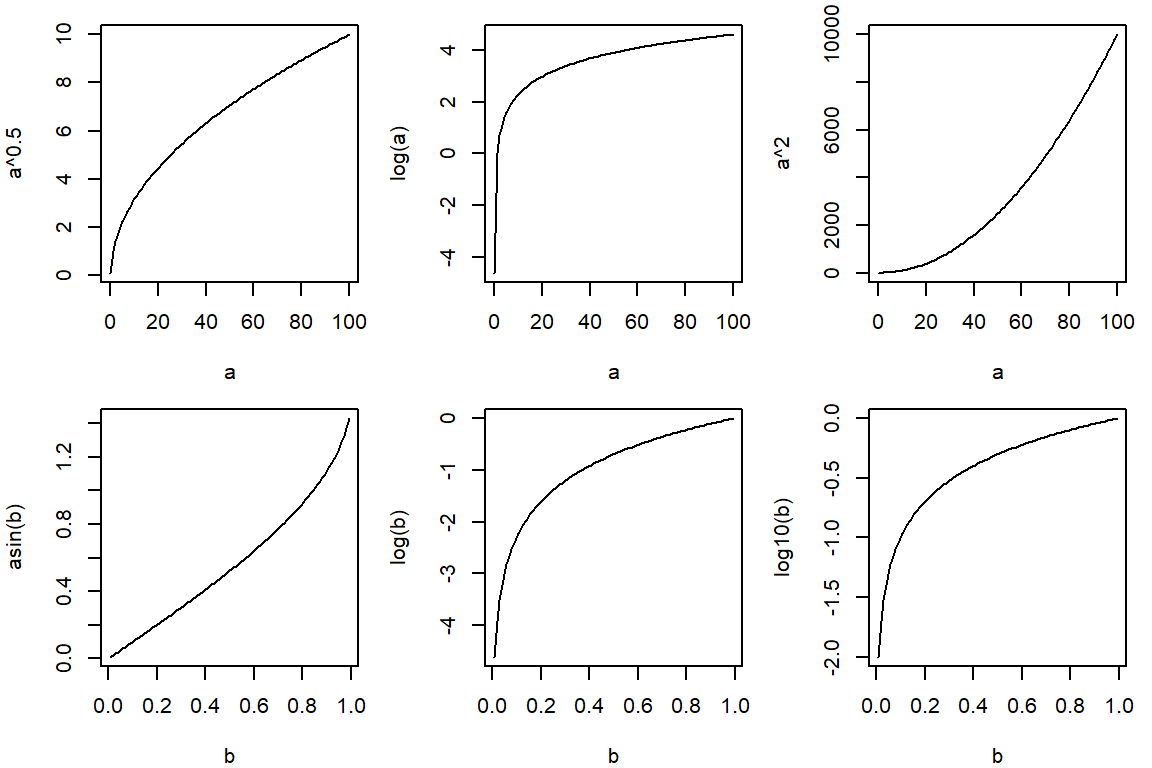
\includegraphics[width=0.7\linewidth,height=0.7\textheight]{_main_files/figure-latex/unnamed-chunk-58-1} \end{center}

\emph{Q95. Using the Radon concentration worksheet, plot the data. Do they look normally distributed?}

\emph{Q96. In your own time,use R to determine the log, square root, and reciprocals (and combinations of all of them: at least one converts the data to approximate normality).}

\begin{Shaded}
\begin{Highlighting}[]
\CommentTok{\# get the Radon data into R; the units are parts per billion}
\NormalTok{readxl}\SpecialCharTok{::}\FunctionTok{excel\_sheets}\NormalTok{(}\StringTok{"data/practical\_3\_4.xlsx"}\NormalTok{) }
\end{Highlighting}
\end{Shaded}

\begin{verbatim}
##  [1] "Cod lengths"           "Shrimps"               "Caffeine"             
##  [4] "Non-parametric shrimp" "Mood shrimp"           "Mood shrimp2"         
##  [7] "Swimming activity"     "Clare's Al data"       "Distribution"         
## [10] "Radon (ppb)"           "Zinc conc"             "Heart-beat,2012"      
## [13] "Sheet1"
\end{verbatim}

\begin{Shaded}
\begin{Highlighting}[]
\CommentTok{\# load the dataset and try some transformations}
\end{Highlighting}
\end{Shaded}

\emph{Q97. Generate a vector of numbers and then use \texttt{sqrt()} on them.}

\begin{center}\rule{0.5\linewidth}{0.5pt}\end{center}

\hypertarget{functions-in-r}{%
\section{Functions in R}\label{functions-in-r}}

Everything that \emph{does} in R is a function. Writing your own functions has many benefits, including keeping your code legible and reducing work for yourself (since any changes need to be done in only one location instead of everywhere you've repeated the same code).

The \texttt{trim\_values} function takes an argument (\texttt{x}), formats it to three digits, and returns the formatted output. Play around with the function to see how it works. We'll use this function to keep our outputted values `clean'. In order to use the function, you must run the code defining it first. You will see your functions listed (alongside your dataframes, vectors, lists, etc) in R-Studio's `Environment' pane.

\begin{Shaded}
\begin{Highlighting}[]
\NormalTok{trim\_values }\OtherTok{\textless{}{-}} \ControlFlowTok{function}\NormalTok{(x) \{}
\NormalTok{  y }\OtherTok{\textless{}{-}} \FunctionTok{format}\NormalTok{(x, }\AttributeTok{digits =} \DecValTok{3}\NormalTok{)}
  \FunctionTok{return}\NormalTok{(y)}
\NormalTok{\} }

\CommentTok{\# After running the code above, we can use the function:}
\FunctionTok{trim\_values}\NormalTok{(}\FloatTok{1.23456}\NormalTok{)}
\end{Highlighting}
\end{Shaded}

\begin{verbatim}
## [1] "1.23"
\end{verbatim}

\begin{Shaded}
\begin{Highlighting}[]
\NormalTok{long\_numbers }\OtherTok{\textless{}{-}} \FunctionTok{rnorm}\NormalTok{(}\DecValTok{3}\NormalTok{, }\DecValTok{2}\NormalTok{, }\DecValTok{1}\NormalTok{)}
\FunctionTok{data.frame}\NormalTok{(}\AttributeTok{orig=}\NormalTok{long\_numbers,}
           \AttributeTok{clean=}\FunctionTok{trim\_values}\NormalTok{(long\_numbers))}
\end{Highlighting}
\end{Shaded}

\begin{verbatim}
##       orig clean
## 1 2.227048  2.23
## 2 1.242831  1.24
## 3 2.121569  2.12
\end{verbatim}

Notice anything strange about the output? The function \texttt{format()} converts the vector from \texttt{numeric} to \texttt{character} to display each value with the same number of characters. The \texttt{digits=3} argument is also taken as a suggestion (kind of like \texttt{breaks} in \texttt{hist()}). Try some of the other options in \texttt{format()} or adjust the \texttt{digits} argument, re-running the function definition each time to see the changes.

\begin{center}\rule{0.5\linewidth}{0.5pt}\end{center}

\hypertarget{the-central-limit-theorem}{%
\section{The central limit theorem}\label{the-central-limit-theorem}}

The central limit theorem states that \textbf{the means of normally distributed data will, themselves, be normally distributed}. In addition, the theorem states that \textbf{the means of data which are NOT normally distributed will be normally distributed if the sample size is sufficiently large}. In this practical we are going to demonstrate this theorem using random data generated from various probability distributions.

\hypertarget{the-distribution-of-means-from-various-data-distributions}{%
\subsection{The distribution of means from various data distributions}\label{the-distribution-of-means-from-various-data-distributions}}

\begin{Shaded}
\begin{Highlighting}[]
\CommentTok{\# Run this code, then adjust the values for obs\_data as you like.}
\CommentTok{\# Play with more distributions if you want: ?stats::distributions}
\NormalTok{obs\_data }\OtherTok{\textless{}{-}} \FunctionTok{c}\NormalTok{(}\FunctionTok{rnorm}\NormalTok{(}\DecValTok{2000}\NormalTok{, }\DecValTok{200}\NormalTok{, }\DecValTok{20}\NormalTok{), }
              \FunctionTok{rnorm}\NormalTok{(}\DecValTok{1500}\NormalTok{, }\DecValTok{100}\NormalTok{, }\DecValTok{20}\NormalTok{), }
              \FunctionTok{rlnorm}\NormalTok{(}\DecValTok{100}\NormalTok{, }\DecValTok{5}\NormalTok{, }\FloatTok{0.5}\NormalTok{),}
              \FunctionTok{rpois}\NormalTok{(}\DecValTok{1000}\NormalTok{, }\DecValTok{15}\NormalTok{), }
              \FunctionTok{rpois}\NormalTok{(}\DecValTok{500}\NormalTok{, }\DecValTok{30}\NormalTok{))}
\NormalTok{xlims }\OtherTok{\textless{}{-}} \FunctionTok{range}\NormalTok{(obs\_data)}

\CommentTok{\# Define size of each sample and the number of sampling repeats}
\NormalTok{sample\_size }\OtherTok{\textless{}{-}} \DecValTok{30}
\NormalTok{num\_samples }\OtherTok{\textless{}{-}} \DecValTok{10000}

\CommentTok{\# Sample num\_samples times from obs\_data, with n = sample\_size for each sample}
\NormalTok{sample\_means }\OtherTok{\textless{}{-}} \FunctionTok{numeric}\NormalTok{(}\AttributeTok{length=}\NormalTok{num\_samples) }\CommentTok{\# initialize an empty vector}
\ControlFlowTok{for}\NormalTok{(i }\ControlFlowTok{in} \DecValTok{1}\SpecialCharTok{:}\NormalTok{num\_samples) \{}
\NormalTok{  sample\_i }\OtherTok{\textless{}{-}} \FunctionTok{sample}\NormalTok{(obs\_data, sample\_size, }\AttributeTok{replace=}\NormalTok{T)}
\NormalTok{  sample\_means[i] }\OtherTok{\textless{}{-}} \FunctionTok{mean}\NormalTok{(sample\_i)}
\NormalTok{\}}

\CommentTok{\# plot observed distribution}
\FunctionTok{par}\NormalTok{(}\AttributeTok{mfrow =} \FunctionTok{c}\NormalTok{(}\DecValTok{2}\NormalTok{, }\DecValTok{2}\NormalTok{))}
\FunctionTok{par}\NormalTok{(}\AttributeTok{mar =} \FunctionTok{c}\NormalTok{(}\DecValTok{5}\NormalTok{, }\DecValTok{2}\NormalTok{, }\DecValTok{2}\NormalTok{, }\DecValTok{2}\NormalTok{)) }
\FunctionTok{hist}\NormalTok{(obs\_data,}
     \AttributeTok{main =} \StringTok{"Raw data distribution"}\NormalTok{,}
     \AttributeTok{sub =} \FunctionTok{paste0}\NormalTok{(}\StringTok{"mean: "}\NormalTok{, }\FunctionTok{trim\_values}\NormalTok{(}\FunctionTok{mean}\NormalTok{(obs\_data)), }
                  \StringTok{", sd: "}\NormalTok{, }\FunctionTok{trim\_values}\NormalTok{(}\FunctionTok{sd}\NormalTok{(obs\_data))),}
     \AttributeTok{breaks =} \DecValTok{30}\NormalTok{, }\AttributeTok{xlab =} \StringTok{"Observed length (cm)"}\NormalTok{, }\AttributeTok{xlim =}\NormalTok{ xlims}
\NormalTok{) }
\FunctionTok{qqnorm}\NormalTok{(obs\_data, }\AttributeTok{main =} \StringTok{"Raw data QQ"}\NormalTok{)}
\FunctionTok{qqline}\NormalTok{(obs\_data)}

\CommentTok{\# plot distribution of sample means}
\FunctionTok{hist}\NormalTok{(sample\_means,}
     \AttributeTok{main =} \FunctionTok{paste0}\NormalTok{(}\StringTok{"Sample distribution, N: "}\NormalTok{, sample\_size),}
     \AttributeTok{sub =} \FunctionTok{paste0}\NormalTok{(}\StringTok{"mean: "}\NormalTok{, }\FunctionTok{trim\_values}\NormalTok{(}\FunctionTok{mean}\NormalTok{(sample\_means)), }
                  \StringTok{", sd: "}\NormalTok{, }\FunctionTok{trim\_values}\NormalTok{(}\FunctionTok{sd}\NormalTok{(sample\_means))),}
     \AttributeTok{breaks =} \DecValTok{30}\NormalTok{, }\AttributeTok{xlab =} \StringTok{"Mean length (cm)"}\NormalTok{, }\AttributeTok{xlim =}\NormalTok{ xlims}
\NormalTok{) }
\FunctionTok{qqnorm}\NormalTok{(sample\_means, }\AttributeTok{main=}\StringTok{"Sample mean QQ"}\NormalTok{)}
\FunctionTok{qqline}\NormalTok{(sample\_means)}
\end{Highlighting}
\end{Shaded}

\begin{figure}

{\centering 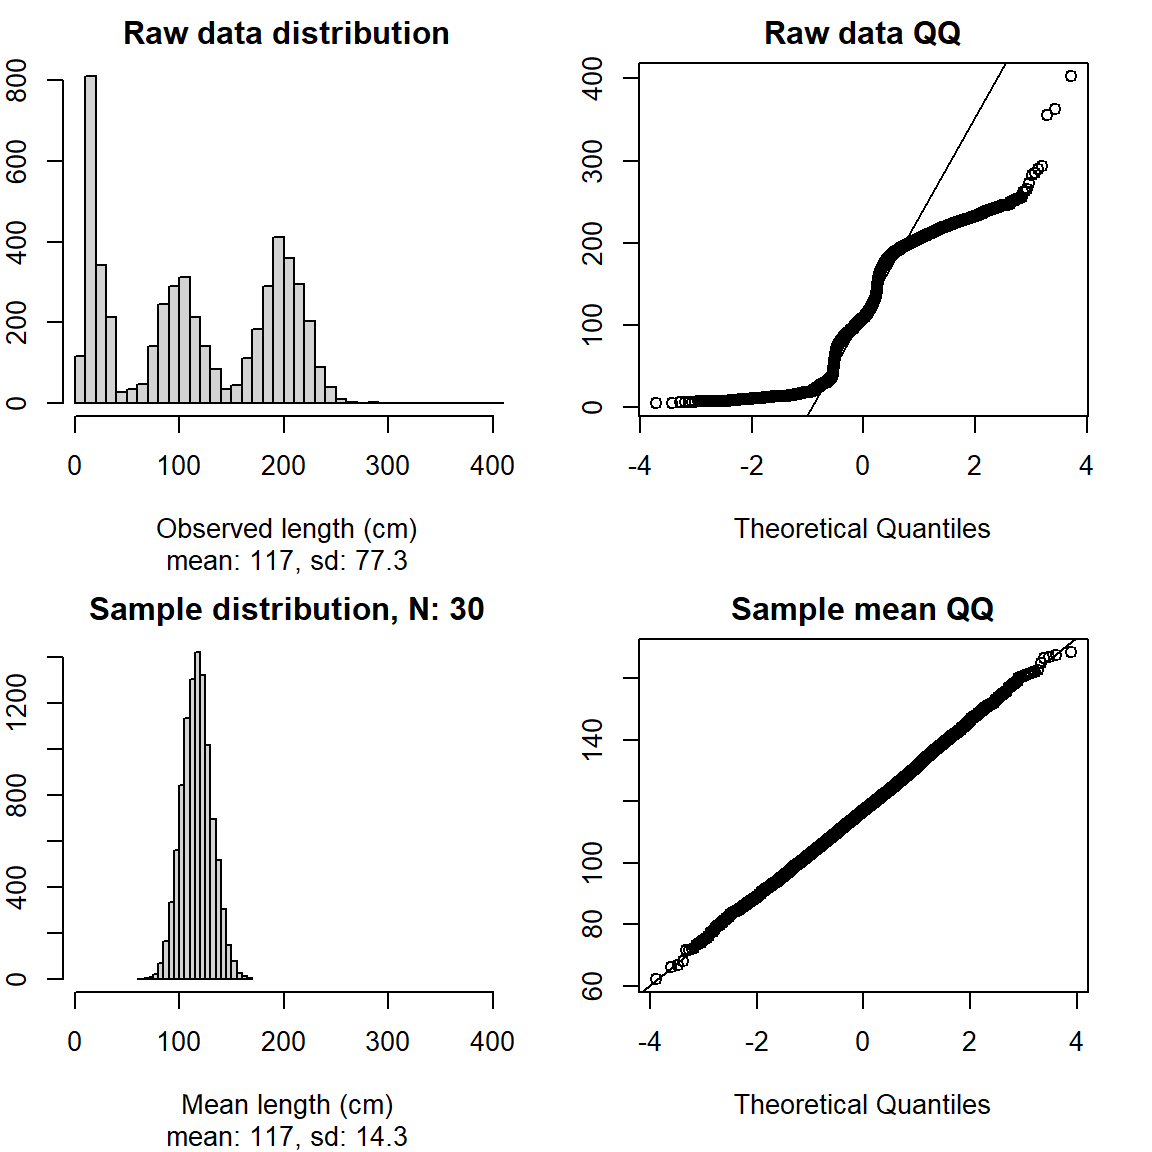
\includegraphics[width=0.7\linewidth,height=0.7\textheight]{_main_files/figure-latex/clt-examp-1} 

}

\caption{The central limit theorem in action (when n>30).}\label{fig:clt-examp}
\end{figure}

\emph{Q98. What do you notice about the location of the mean as a function of N?}

\emph{Q99. What do you notice about the spread around the mean in each group as a function of sample size -- why did the pattern you have observed occur?}

You are witnessing the central limit theorem in action -- the means of normally distributed numbers are, themselves, normally distributed, and the means of non-normally distributed numbers are \emph{also} normally distributed provided the sample size is large enough. Note the relationship between the sample size and the range of values for the sample mean. How does the standard deviation of \texttt{sample\_means} change with changes in \texttt{sample\_size}?.

\begin{center}\rule{0.5\linewidth}{0.5pt}\end{center}

\hypertarget{the-standard-error-of-the-mean}{%
\section{The standard error of the mean}\label{the-standard-error-of-the-mean}}

The standard error of the mean is simply the standard deviation of sample means, of a given sample size, taken from a population. That is, it is the standard deviations calculated in the lower histogram in Fig. \ref{fig:clt-examp}. It is calculated as \(SE_{\bar{y}} = \frac{sd(y)}{\sqrt{n}}\).

\begin{Shaded}
\begin{Highlighting}[]
\FunctionTok{library}\NormalTok{(tidyverse)}
\CommentTok{\# Simulate a normally distributed population with mean mu and sd sigma}
\NormalTok{mu }\OtherTok{\textless{}{-}} \DecValTok{10}
\NormalTok{sigma }\OtherTok{\textless{}{-}} \DecValTok{2}
\NormalTok{sim\_obs }\OtherTok{\textless{}{-}} \FunctionTok{rnorm}\NormalTok{(}\DecValTok{10000}\NormalTok{, mu, sigma)}

\CommentTok{\# Draw samples}
\NormalTok{sample\_size }\OtherTok{\textless{}{-}} \FunctionTok{c}\NormalTok{(}\DecValTok{2}\NormalTok{, }\DecValTok{10}\NormalTok{, }\DecValTok{30}\NormalTok{, }\DecValTok{100}\NormalTok{) }\CommentTok{\# size of each sample}
\NormalTok{num\_samples }\OtherTok{\textless{}{-}} \DecValTok{1000} \CommentTok{\# number of samples (=repeats) for each sample size}

\NormalTok{sample\_mean\_df }\OtherTok{\textless{}{-}} \FunctionTok{tibble}\NormalTok{(}\AttributeTok{N=}\FunctionTok{rep}\NormalTok{(sample\_size, }\AttributeTok{each =}\NormalTok{ num\_samples),}
                         \AttributeTok{id=}\FunctionTok{rep}\NormalTok{(}\DecValTok{1}\SpecialCharTok{:}\NormalTok{num\_samples, }\AttributeTok{times =} \FunctionTok{length}\NormalTok{(sample\_size))) }\SpecialCharTok{|\textgreater{}}
  \FunctionTok{mutate}\NormalTok{(}\AttributeTok{sample\_mean=}\DecValTok{0}\NormalTok{)}

\ControlFlowTok{for}\NormalTok{(i }\ControlFlowTok{in} \DecValTok{1}\SpecialCharTok{:}\FunctionTok{nrow}\NormalTok{(sample\_mean\_df)) \{}
\NormalTok{  sample\_i }\OtherTok{\textless{}{-}} \FunctionTok{sample}\NormalTok{(sim\_obs, sample\_mean\_df}\SpecialCharTok{$}\NormalTok{N[i])}
\NormalTok{  sample\_mean\_df}\SpecialCharTok{$}\NormalTok{sample\_mean[i] }\OtherTok{\textless{}{-}} \FunctionTok{mean}\NormalTok{(sample\_i)}
\NormalTok{\}}
\end{Highlighting}
\end{Shaded}

\begin{Shaded}
\begin{Highlighting}[]
\NormalTok{sample\_mean\_df }\SpecialCharTok{|\textgreater{}}
  \FunctionTok{mutate}\NormalTok{(}\AttributeTok{N=}\FunctionTok{factor}\NormalTok{(N, }\AttributeTok{levels=}\FunctionTok{unique}\NormalTok{(N))) }\SpecialCharTok{|\textgreater{}}
  \FunctionTok{ggplot}\NormalTok{(}\FunctionTok{aes}\NormalTok{(N, sample\_mean)) }\SpecialCharTok{+} 
  \FunctionTok{geom\_hline}\NormalTok{(}\AttributeTok{yintercept=}\NormalTok{mu, }\AttributeTok{linetype=}\DecValTok{3}\NormalTok{) }\SpecialCharTok{+}
  \FunctionTok{geom\_violin}\NormalTok{(}\AttributeTok{scale=}\StringTok{"width"}\NormalTok{, }\AttributeTok{draw\_quantiles=}\FunctionTok{c}\NormalTok{(}\FloatTok{0.025}\NormalTok{, }\FloatTok{0.5}\NormalTok{, }\FloatTok{0.975}\NormalTok{), }\AttributeTok{fill=}\ConstantTok{NA}\NormalTok{) }\SpecialCharTok{+}
  \FunctionTok{geom\_jitter}\NormalTok{(}\AttributeTok{alpha=}\FloatTok{0.2}\NormalTok{, }\AttributeTok{shape=}\DecValTok{1}\NormalTok{, }\AttributeTok{width=}\FloatTok{0.05}\NormalTok{) }\SpecialCharTok{+} 
  \FunctionTok{labs}\NormalTok{(}\AttributeTok{x=}\StringTok{"Sample size"}\NormalTok{, }\AttributeTok{y=}\FunctionTok{paste}\NormalTok{(}\StringTok{"Means of"}\NormalTok{, num\_samples, }\StringTok{"simulated samples"}\NormalTok{)) }\SpecialCharTok{+}
  \FunctionTok{theme\_classic}\NormalTok{()}
\end{Highlighting}
\end{Shaded}

\begin{figure}

{\centering 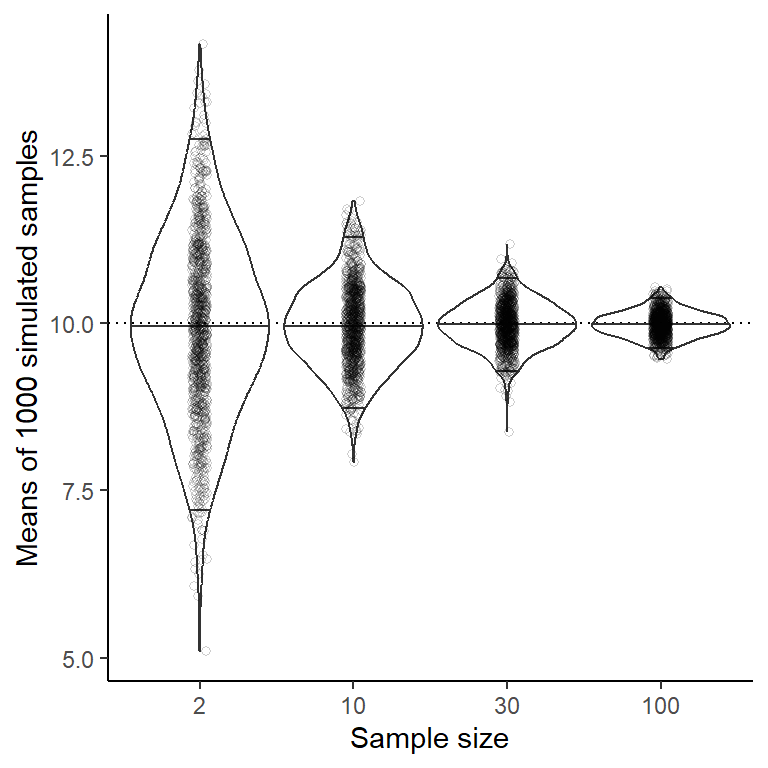
\includegraphics[width=0.5\linewidth,height=0.5\textheight]{_main_files/figure-latex/SEM-fig-1} 

}

\caption{Simulated sample means.}\label{fig:SEM-fig}
\end{figure}

\emph{Q100. Calculate the theoretical standard error of the means for each \texttt{sample\_size} given \texttt{sigma} and compare this with your actual standard error (=standard deviation) of sample means}

\emph{Q101. Given what you know about the CLT, how does this change with non-normally distributed data? Try changing \texttt{rnorm()} to \texttt{rpois()}}

\emph{Q102. Change \texttt{sigma} and \texttt{sample\_size} and check that the standard error estimates are in line with their true values (i.e.~as determined by using the standard error formula).}

\begin{center}\rule{0.5\linewidth}{0.5pt}\end{center}

\hypertarget{normal-approximations-for-other-distributions}{%
\section{Normal approximations for other distributions}\label{normal-approximations-for-other-distributions}}

In earlier exercises you saw that the Poisson distribution could be used to approximate the binomial distribution. In a conceptually similar way, the normal distribution can be used to approximate the Poisson model.

\hypertarget{the-normal-approximation-of-the-poisson-distribution}{%
\subsection{The Normal approximation of the Poisson distribution}\label{the-normal-approximation-of-the-poisson-distribution}}

Recall that the Poisson model takes only one parameter, the mean, and that where a variable is Poisson distributed the variance equals the mean. So if we have a variable \(y \sim Pois(10)\), the mean (say density per quadrat) is 10 and so is the variance. We now have the two parameters that define the normal distribution (the mean and variance).

\emph{Q103. For} \(y \sim Pois(10)\) \emph{write the equivalent normal distribution in standard notation.}

As a rough guideline, a normal approximation is reasonable if \(\lambda \geq 30\). So \(y \sim Pois(10)\) should not be approximated by the normal distribution while \(y \sim Pois(30)\) could be. However, it is generally preferable to use the natural distribution for your data (e.g., a Poisson distribution for counts). The normal distribution is beneficial in some cases, but this is increasingly less so with modern methods.

\emph{Q104. For a Poisson distribution} \(y \sim Pois(40)\) \emph{define the normal approximation in the standard way.}

\emph{Q105. Using R and referring Practical @ref(bin\_pois), calculate} \(P(y_i \leq 35)\) \emph{from} \(y \sim Pois(40)\) \emph{(Ans = 0.242)}

\emph{Q106. Using R, calculate} \(P(y_i < 35)\) \emph{from the above normal approximation of the Poisson distribution (Ans = 0.215).}

\emph{Q107. What do you think of the normal approximation?}

\emph{Q108. Evaluate} \(P(y_i<3\ |\ \lambda=5)\) \emph{using the Poisson model and its normal approximation.}

\hypertarget{the-normal-approximation-of-the-binomial-distribution}{%
\subsection{The normal approximation of the binomial distribution}\label{the-normal-approximation-of-the-binomial-distribution}}

Whilst we accept the fundamental difference between continuous and discrete data, in making continuous-variable measurements we inevitably allocate each measurement to a single measurement category (we are limited by our ability to measure, eg. to the nearest millimeter if using a ruler). If we wish to treat a continuous variable as a continuous variable, the number of categories between the smallest and largest measurement should be a minimum of \textasciitilde30 (the upper limit doesn't matter so much but there is no need to \textgreater300). For example, suppose we were measuring fish-lengths and the min was 20 cm and the max 40 cm. That means there are 20 x 1 cm measurement units between them. This falls under our 30 unit minimum -- measuring to the nearest cm would not be adequate. There are, however, 40 x 0.5 cm units between them so we could measure to the nearest 0.5 cm (we would probably use 0.1 cm though). But, even if we measure to the correct degree of precision, we are still categorising the lengths. For example, a fish of 20.5 cm actually means we think that fish was between 20.45 and 20.55 cm.

What is the point of this? Well, if you have a binomially distributed variable where \(n\), the number of trials, is sufficiently large (meaning the number of outcomes is large too) then the binomial distribution begins to look like the normal distribution, particularly where \(p\) is somewhere near 0.5. The general guideline is that where the number of trials multiplied by the smaller of the probability of success (\(p\)) or the probability of failure (\(q=1-p\)) is greater than 5 then we can reasonably use the normal distribution to model the data (i.e.~both \(n*p > 5\) and \(n*(1-p) > 5\)).

Turtles lay clutches of 40 eggs. We might be interested in predicting the number of male and female offspring. Assume the proportion that are male is 0.5. Our investigation stems from the observation that several clutches of eggs, on a particular island, contained only 10 males. We might wonder how unlikely this was by chance, assuming \(P(male)=0.5\).

\emph{Q109. Referring to Practical @ref\{bin\_pois\} if necessary, use the binomial model, calculate how unusual (i.e.~the probability) it is to get} \(\leq 10\) \emph{males.}

\emph{Q110. Plot your probability (i.e.~from 0 -- 40 males) as a bar graph. Comment on its shape.}

The variance of a binomially distributed variable is simply \(n*p*q\).

\emph{Q111. Calculate the mean and variance of this population.}

\emph{Q112. Are} \(n*p\) \emph{and} \(n*(p-1)\) \emph{both \textgreater5?}

\emph{Q113. Given these two variables, specify the equivalent normal distribution.}

We have the `real' distribution \(y \sim Binom(40,0.5)\) and its normal approximation. We ask what is \(P(y_i \leq 10)\) given \(y \sim Binom(40, 0.5)\) and given \(y \sim Norm(20, 10)\).

\emph{Q114. Calculate the Z score for 10 males then find the probability of making this observation.}

\emph{Q115. How do the values from the different models compare?}

\begin{center}\rule{0.5\linewidth}{0.5pt}\end{center}

\hypertarget{conclusions-2}{%
\section{Conclusions}\label{conclusions-2}}

The normal distribution is central to statistics. A huge variety of observations are reasonably approximated by the normal distribution (or can be made to be normally distributed through transformation).

The normal distribution can be used to assess the likelihood of a given observation, if we know the population mean and standard deviation from which it came. Furthermore, given our knowledge of the population parameter (mean and variance) we can determine values which define intervals on that population. Frequently scientists determine the values that bound 95\% of their data.

The central limit theorem says that sample means taken from a normally distributed population will themselves be normally distributed and, in addition, means of sufficiently large samples will also be normally distributed even where the original data are not normally distributed (the sample size required depends on the extent of the skew in the original data).

The normal distribution is a good approximation of the Poisson distribution when lambda is large and the binomial model where the number of trials is large and the probability of success around 0.5 (i.e.~the distribution of values is not too skewed).

\hypertarget{t-test}{%
\chapter{t-tests \& confidence intervals}\label{t-test}}

The goal of science is to understand nature (i.e.~everything!). In order to do that, we want to know the values of population parameters (e.g.~the mean size of barnacles on the back-beach, the variance in fail-rate of a machine component, the maximum satelite signal strength per satelite transect, the mean size of a fisher's catch). However, we are usually limited in our capacity to measure entire populations due to logistical/time/money constraints so we take a (random) sample, and infer from that sample to our population of interest. This is statistical inference and it's based on our statistical models of the world.

When we take a random sample we can never know how well it reflects the population. For example, our random sample of barnacles might contain (by chance alone) mostly big ones, or barnacles that varied considerably (or negligibly) in size. The t-distribution is similar to the normal distribution, but it accounts for this added uncertainty. This enables us to estimate the probability that a given sample came from a population with any given mean (with caveats). The t-distribution also enables us to put confidence intervals around the mean of our sample, and gives us some idea of the range of values of the mean that are likely.

The t-distribution models the chances of making observations from a given population where the population parameters are estimated from your random sample. The t statistic is calculated in the same way as the Z score for samples, but the expected scores follow the t-distribution (instead of the normal distribution) which accounts for sampling uncertainty. As the sample size gets smaller we get increasingly less confident about the reliability of the population parameter estimates and the t-distribution becomes less like the normal distribution (Fig. \ref{fig:t-vs-norm}). The shape of the t-distribution depends on the \emph{degrees of freedom} (\(df = \nu = N-1\)). There is more guidance on the t-distribution, and links to other sources on Brightspace.

\begin{figure}

{\centering 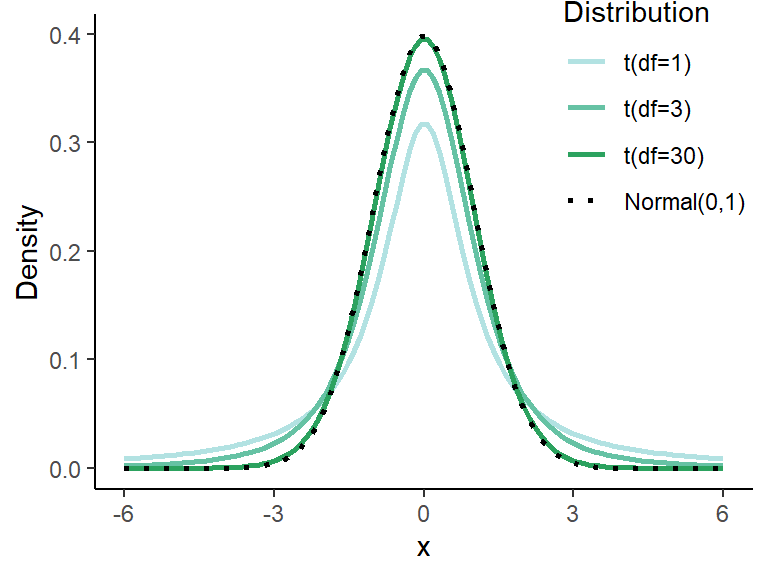
\includegraphics[width=0.5\linewidth,height=0.5\textheight]{_main_files/figure-latex/t-vs-norm-1} 

}

\caption{Comparison of different t-distributions (note that t with 30 df is nearly identical to the normal distribution).}\label{fig:t-vs-norm}
\end{figure}

\emph{Q116. Would you feel as confident about basing an estimate of the heights of the lab population on a sample of 2 compared with a sample of 50?}

\emph{Q117. How does sample size affect the reliability of our population parametr estimates?}

\hypertarget{single-sample-t-tests}{%
\section{Single sample t-tests}\label{single-sample-t-tests}}

This is analogous to the calculation of Z scores and enables us to determine how unlikely our sample mean is, given any hypothesised mean. However, before using any parametric tests such as t-tests, we need to assure ourselves that the model assumptions are reasonably met. Note that t-tests, as illustrated here, are not testing null-hypotheses.

Imagine we are fisheries inspectors and have sampled the cod landed by a fishing boat called the `The Evening Star'. We know that the mean size of the cod landed should be greater than 36.6 cm. We need to assess how likely it is that our sampled cod come from a population (of landed fish) where the mean actually is \(\geq\) 36.6 cm. We are testing the hypothesis that there is one `population' of legally landed cod, and the Evening Star's cod are a part of that population. We use the t-distribution to assess the probability the Evening Star cod are drawn from the legally-landed cod population. If this probability is low then we might speculate that the cod are, in fact, drawn from a different population (i.e., that the boat is using illegal gear).

We do not know the population mean or standard deviation of the population from which the cod were caught and hence cannot use a normal distribution to model the likelihood of observing any particular value.

Before starting problems like this always state your hypotheses. You should (unless instructed otherwise) state both the null and alternative hypothesis. Here we are wondering whether the mean cod size on the Evening Star is \(<\) 36.6 cm. The hypothesis should be worded thus:

\textbf{H\textsubscript{0} (the null hypothesis):} The true value of the mean of the Evening Star cod is \(\geq\) 36.6 cm (\(\mu \geq\) 36.6 cm).

\textbf{H\textsubscript{1} (the alternative hypothesis):} The true value of the mean Evening Star cod is less than 36.6 cm (\(\mu <\) 36.6 cm).

We use the t-test to determine the probability of drawing the Evening Star sample from a population where the true mean is 36.6 cm or greater.

\emph{Q118. Given the hypothesis, is this one or two tailed test?}

We collect a sample of 20 fish (found in the worksheet `Cod lengths'). The sample size is \(<\) 30 so we can't assume that the means will be normally distributed under the CLT. We can check the normality assumption by plotting the data using a `normality' plot or `QQ-plot' (Fig. \ref{fig:cod-qq}).

\begin{Shaded}
\begin{Highlighting}[]
\FunctionTok{library}\NormalTok{(readxl)}
\NormalTok{cod\_df }\OtherTok{\textless{}{-}} \FunctionTok{read\_excel}\NormalTok{(}\StringTok{"data/practical\_3\_4.xlsx"}\NormalTok{, }\AttributeTok{sheet =} \StringTok{"Cod lengths"}\NormalTok{)}
\FunctionTok{str}\NormalTok{(cod\_df)}
\end{Highlighting}
\end{Shaded}

\begin{verbatim}
## tibble [20 x 1] (S3: tbl_df/tbl/data.frame)
##  $ CodLength_cm: num [1:20] 34.1 35.6 36.1 34.6 38.3 35 36.8 38 34.4 35.5 ...
\end{verbatim}

\begin{Shaded}
\begin{Highlighting}[]
\FunctionTok{qqnorm}\NormalTok{(cod\_df}\SpecialCharTok{$}\NormalTok{CodLength\_cm, }\AttributeTok{main =} \ConstantTok{NULL}\NormalTok{)}
\FunctionTok{qqline}\NormalTok{(cod\_df}\SpecialCharTok{$}\NormalTok{CodLength\_cm)}
\end{Highlighting}
\end{Shaded}

\begin{figure}

{\centering 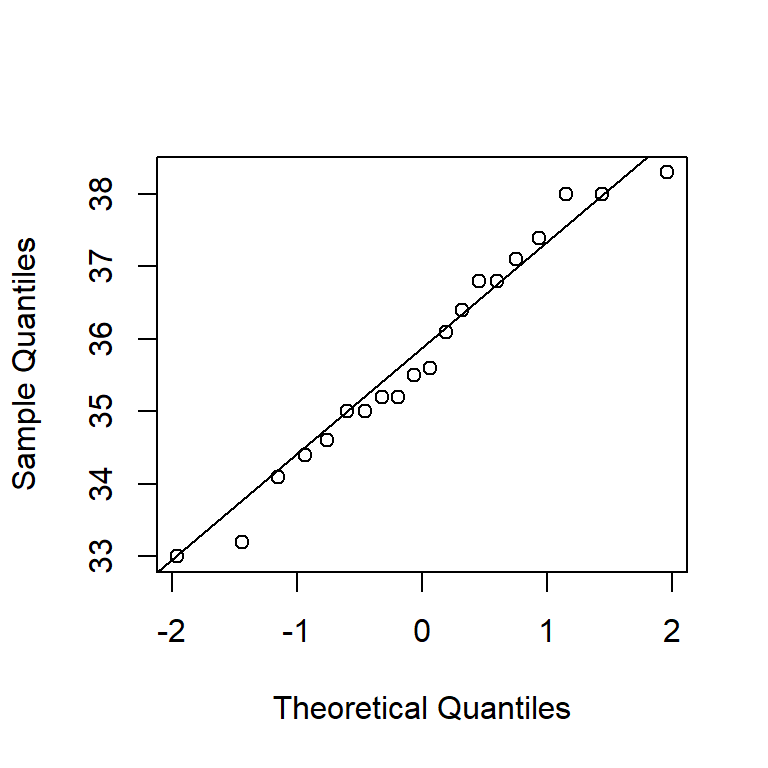
\includegraphics[width=0.5\linewidth,height=0.5\textheight]{_main_files/figure-latex/cod-qq-1} 

}

\caption{QQ-plot for the sample of code from the Evening Star.}\label{fig:cod-qq}
\end{figure}

\emph{Q119. Do you think the normality assumption reasonable?}

\emph{Q120. What parameter are we actually trying to understand/model? How does the distribution of this parameter change with sample size (think CLT)?}

Now we wish to assess how likely our sample is to have been drawn from a population where the mean actually is 36.6 cm. If the ES mean is less than the `legal' mean and it is `unlikely' to have been drawn from the legal population we might wonder if the mean of true Evening Star landed cod population is \textless36.6 cm and decide to prosecute the skipper.

\emph{Q121. Use R to calculate summary statistics (mean and standard deviation/standard error of the mean) for the cod sample data (as per results below).}

\begin{Shaded}
\begin{Highlighting}[]
\FunctionTok{cat}\NormalTok{(}\StringTok{"Mean:"}\NormalTok{, }\FunctionTok{mean}\NormalTok{(cod\_df}\SpecialCharTok{$}\NormalTok{CodLength\_cm))}
\FunctionTok{cat}\NormalTok{(}\StringTok{"SD:"}\NormalTok{, }\FunctionTok{sd}\NormalTok{(cod\_df}\SpecialCharTok{$}\NormalTok{CodLength\_cm))}
\FunctionTok{cat}\NormalTok{(}\StringTok{"Var:"}\NormalTok{, }\FunctionTok{var}\NormalTok{(cod\_df}\SpecialCharTok{$}\NormalTok{CodLength\_cm))}
\FunctionTok{cat}\NormalTok{(}\StringTok{"N:"}\NormalTok{, }\FunctionTok{length}\NormalTok{(cod\_df}\SpecialCharTok{$}\NormalTok{CodLength\_cm))}
\end{Highlighting}
\end{Shaded}

\begin{verbatim}
## Mean: 35.785SD: 1.549966Var: 2.402395N: 20
\end{verbatim}

\emph{Q122. Determine the standard error of the mean (see Chapter \ref{appendix} if necessary)}

\begin{Shaded}
\begin{Highlighting}[]
\FunctionTok{sd}\NormalTok{(cod\_df}\SpecialCharTok{$}\NormalTok{CodLength\_cm) }\SpecialCharTok{/} \FunctionTok{sqrt}\NormalTok{(}\FunctionTok{length}\NormalTok{(cod\_df}\SpecialCharTok{$}\NormalTok{CodLength\_cm))}
\end{Highlighting}
\end{Shaded}

\begin{verbatim}
## [1] 0.3465829
\end{verbatim}

\emph{Q123. Now manually calculate the t statistic for this sample and determine the probablity of observing your data assuming that the mean of the population was actually 36.6 cm.}

\begin{Shaded}
\begin{Highlighting}[]
\NormalTok{T\_stat }\OtherTok{\textless{}{-}}\NormalTok{ (}\FunctionTok{mean}\NormalTok{(cod\_df}\SpecialCharTok{$}\NormalTok{CodLength\_cm) }\SpecialCharTok{{-}} \FloatTok{36.6}\NormalTok{) }\SpecialCharTok{/} 
\NormalTok{  (}\FunctionTok{sd}\NormalTok{(cod\_df}\SpecialCharTok{$}\NormalTok{CodLength\_cm) }\SpecialCharTok{/} \FunctionTok{sqrt}\NormalTok{(}\FunctionTok{length}\NormalTok{(cod\_df}\SpecialCharTok{$}\NormalTok{CodLength\_cm)))}
\end{Highlighting}
\end{Shaded}

\emph{Q124. How does this value compare to the expectation under the null hypothesis? Use \texttt{pt()}.}

Remember you are conducting a single-tailed test here, so you need to look-up your t-statistic at an \(\alpha\) rate of double your P value of interest (so if you are setting a 95\% CI you need to look-up \(\alpha\) value of 0.100).

\emph{Q125. Check you answer against that given by R.}

\begin{Shaded}
\begin{Highlighting}[]
\FunctionTok{t.test}\NormalTok{(cod\_df}\SpecialCharTok{$}\NormalTok{CodLength\_cm, }\AttributeTok{mu =} \FloatTok{36.6}\NormalTok{, }\AttributeTok{alternative =} \StringTok{"less"}\NormalTok{,}
       \AttributeTok{conf.level =} \FloatTok{0.95}\NormalTok{, }\AttributeTok{var.equal =} \ConstantTok{TRUE}\NormalTok{)}
\end{Highlighting}
\end{Shaded}

\begin{verbatim}
## 
##  One Sample t-test
## 
## data:  cod_df$CodLength_cm
## t = -2.3515, df = 19, p-value = 0.01482
## alternative hypothesis: true mean is less than 36.6
## 95 percent confidence interval:
##      -Inf 36.38429
## sample estimates:
## mean of x 
##    35.785
\end{verbatim}

Hopefully your manually calculated t statistic and the one generated by R match. The p-value given by R is exact i.e.~there is a probability of 0.014819 that a sample of 20 cod with mean of 35.785 cm would be drawn from a legally landed cod population where the true mean was 36.6 cm or more (assuming model assumptions are met).

\emph{Q126. Can we now confidently send the skipper to jail?}

Remember the confidence interval relates to future (often hypothetical) observations, not an observation that has been made. Confidence intervals are notoriously difficult to define and and are often incorrectly used. BrightSpace has numerous resources to help you.

Evaluating evidence is a central part of statistcal analysis/modelling. In this example, assume you are evaluating whether a fishers catch is `surprisingly' small (e.g.~that the fisher is using an illegal net). If you don't believe the fisher (i.e that the fish sample was not drawn from a population of fish with a mean of 36.6 cm) then she goes to jail. If you do believe her, but she was fishing illegally, she avoids jail. In these circumstances you should set-out your P-value thresholds ahead of getting the data. For the moment, assume we set the P-value (\(\alpha\) value) threshold at 0.05. In this scenario, where we have two clear competing hypotheses, we are in the realm of `Neyman-Pearson's' decision theory (not in Fisher's hypothesis significance testing approach; see P-value lecture).

\emph{Q127. Given the P value, do you reject the null hypothesis?}

\emph{Q128. If you had set alpha at 0.01 would you reject the null hypothesis?}

\emph{Q129. If you set alpha at 0.01, rather than 0.05, what type of error are you reducing and what type of error are you increasing?}

Now to play around with some random data that you generate yourself. We generate 100 random numbers drawn from X, where \(X \sim Norm(100, 10)\).

\emph{Q130. What is your standard deviation in this model?}

\emph{Q131. What does the symbol `\textasciitilde{}' mean?}

We calculate summary statistics for this randomly generated dataset. Note that in this case, we \emph{know} the population parameters.

\begin{Shaded}
\begin{Highlighting}[]
\NormalTok{num\_iter }\OtherTok{\textless{}{-}} \DecValTok{3}
\NormalTok{sample\_size }\OtherTok{\textless{}{-}} \DecValTok{3}
\NormalTok{mu }\OtherTok{\textless{}{-}} \DecValTok{100}
\NormalTok{sigma }\OtherTok{\textless{}{-}} \DecValTok{10}

\FunctionTok{paste0}\NormalTok{(}\StringTok{"True mean: "}\NormalTok{, mu, }\StringTok{", true sd: "}\NormalTok{, sigma)}
\ControlFlowTok{for}\NormalTok{ (i }\ControlFlowTok{in} \DecValTok{1}\SpecialCharTok{:}\NormalTok{num\_iter) \{}
\NormalTok{  sample\_i }\OtherTok{\textless{}{-}} \FunctionTok{rnorm}\NormalTok{(}\AttributeTok{n =}\NormalTok{ sample\_size, }\AttributeTok{mean =}\NormalTok{ mu, }\AttributeTok{sd =}\NormalTok{ sigma)}
\NormalTok{  sample\_mean }\OtherTok{\textless{}{-}} \FunctionTok{signif}\NormalTok{(}\FunctionTok{mean}\NormalTok{(sample\_i), }\DecValTok{4}\NormalTok{)}
\NormalTok{  sample\_sd }\OtherTok{\textless{}{-}} \FunctionTok{signif}\NormalTok{(}\FunctionTok{sd}\NormalTok{(sample\_i), }\DecValTok{4}\NormalTok{)}
  \FunctionTok{print}\NormalTok{(}\FunctionTok{paste0}\NormalTok{(}\StringTok{"Sample "}\NormalTok{, i, }\StringTok{" mean:"}\NormalTok{, sample\_mean, }\StringTok{", sd: "}\NormalTok{, sample\_sd))}
\NormalTok{\}}
\end{Highlighting}
\end{Shaded}

\begin{verbatim}
## [1] "True mean: 100, true sd: 10"
## [1] "Sample 1 mean:100.1, sd: 14.63"
## [1] "Sample 2 mean:107.9, sd: 5.05"
## [1] "Sample 3 mean:100.9, sd: 13.9"
\end{verbatim}

Note: these are random samples, so the values will be different each time you run the code. However, R uses pseudo-random number generation. Use \texttt{set.seed()} for fully replicable code.

\emph{Q132. Is there a discrepancy between the population parameters you defined and the actual mean and variance that are estimated from the samples?}

Your answer to the above should be yes. You know there is a discrepancy because you know the true parameters. In most real life situations you do not know the true population mean and variance. You can only sample them. If your sample is very large (and representative) then you can generate a very good estimate of those population parameters. However, as your sample size is reduced, the reliability of your estimate decreases. Look at the random numbers you've generated. Get a sense for where most of the numbers lie with \texttt{sigma=10}. To output your sample, just run \texttt{sample\_i}.

The t-distribution is the distribution of values you get when you subtract sample means from the true mean and standardise by the sample standard error (i.e., \(\frac{\bar{x} - \mu}{SE_{\bar{x}}}\)). Think about this and relate it to the formula for determining single-sample T-statistics and what the critical values actually are that are tabulated in Table 7.

The code below simulates repeated samples from a population with \(y \sim Norm(\mu, \sigma)\). Each sample takes \texttt{sample\_size} individuals, with \texttt{num\_samples} unique samples. For each sample \texttt{i}, the t-statistic is calculated and stored in \texttt{T\_sample{[}i{]}}. Fig. \ref{fig:t-stat-hist} shows the distribution of \texttt{T\_sample} (the histogram) with the corresponding t-distribution (df=\texttt{sample\_size\ -\ 1}) as the solid line and a standard normal distribution as the dotted line. Play with the values for \texttt{sample\_size} below to see how the shapes change.

\begin{Shaded}
\begin{Highlighting}[]
\NormalTok{mu }\OtherTok{\textless{}{-}} \DecValTok{10} \CommentTok{\# population mean}
\NormalTok{sigma }\OtherTok{\textless{}{-}} \FloatTok{0.5} \CommentTok{\# population sd}
\NormalTok{num\_samples }\OtherTok{\textless{}{-}} \FloatTok{1e5} \CommentTok{\# number of samples}
\NormalTok{sample\_size }\OtherTok{\textless{}{-}} \DecValTok{3} \CommentTok{\# size of each sample}
\NormalTok{T\_sample }\OtherTok{\textless{}{-}} \FunctionTok{numeric}\NormalTok{(sample\_size) }\CommentTok{\# sample t statistic}

\ControlFlowTok{for}\NormalTok{ (i }\ControlFlowTok{in} \DecValTok{1}\SpecialCharTok{:}\NormalTok{num\_samples) \{}
\NormalTok{  sample\_i }\OtherTok{\textless{}{-}} \FunctionTok{rnorm}\NormalTok{(sample\_size, mu, sigma)}
\NormalTok{  sample\_SEM }\OtherTok{\textless{}{-}} \FunctionTok{sd}\NormalTok{(sample\_i) }\SpecialCharTok{/} \FunctionTok{sqrt}\NormalTok{(sample\_size)}
\NormalTok{  T\_sample[i] }\OtherTok{\textless{}{-}}\NormalTok{ (}\FunctionTok{mean}\NormalTok{(sample\_i) }\SpecialCharTok{{-}}\NormalTok{ mu) }\SpecialCharTok{/}\NormalTok{ (sample\_SEM)}
\NormalTok{\}}

\FunctionTok{curve}\NormalTok{(}\FunctionTok{dnorm}\NormalTok{(x, }\DecValTok{0}\NormalTok{, }\DecValTok{1}\NormalTok{), }\AttributeTok{from =} \SpecialCharTok{{-}}\DecValTok{6}\NormalTok{, }\AttributeTok{to =} \DecValTok{6}\NormalTok{, }\AttributeTok{lty =} \DecValTok{2}\NormalTok{, }
      \AttributeTok{xlab =} \StringTok{"Simulated t{-}statistics"}\NormalTok{, }\AttributeTok{ylab =} \StringTok{"Density"}\NormalTok{,}
      \AttributeTok{main =} \FunctionTok{paste}\NormalTok{(}\StringTok{"t{-}statistics of"}\NormalTok{, }\FunctionTok{format}\NormalTok{(}\FloatTok{1e5}\NormalTok{, }\AttributeTok{big.mark=}\StringTok{","}\NormalTok{, }\AttributeTok{scientific=}\NormalTok{F), }
                   \StringTok{"samples, each with N ="}\NormalTok{, sample\_size))}
\FunctionTok{hist}\NormalTok{(T\_sample, }\AttributeTok{freq =}\NormalTok{ F, }\AttributeTok{add =}\NormalTok{ T, }\AttributeTok{col =} \FunctionTok{rgb}\NormalTok{(}\DecValTok{1}\NormalTok{, }\DecValTok{0}\NormalTok{, }\DecValTok{0}\NormalTok{, }\FloatTok{0.25}\NormalTok{), }
     \AttributeTok{breaks =} \FunctionTok{seq}\NormalTok{(}\FunctionTok{floor}\NormalTok{(}\FunctionTok{min}\NormalTok{(T\_sample)), }\FunctionTok{ceiling}\NormalTok{(}\FunctionTok{max}\NormalTok{(T\_sample)), }\AttributeTok{by=}\FloatTok{0.2}\NormalTok{))}
\FunctionTok{curve}\NormalTok{(}\FunctionTok{dnorm}\NormalTok{(x, }\DecValTok{0}\NormalTok{, }\DecValTok{1}\NormalTok{), }\AttributeTok{from =} \SpecialCharTok{{-}}\DecValTok{6}\NormalTok{, }\AttributeTok{to =} \DecValTok{6}\NormalTok{, }\AttributeTok{add =}\NormalTok{ T, }\AttributeTok{lty =} \DecValTok{2}\NormalTok{)}
\FunctionTok{curve}\NormalTok{(}\FunctionTok{dt}\NormalTok{(x, sample\_size }\SpecialCharTok{{-}} \DecValTok{1}\NormalTok{), }\AttributeTok{from =} \SpecialCharTok{{-}}\DecValTok{6}\NormalTok{, }\AttributeTok{to =} \DecValTok{6}\NormalTok{, }\AttributeTok{add =}\NormalTok{ T)}
\FunctionTok{legend}\NormalTok{(}\StringTok{"topright"}\NormalTok{, }\AttributeTok{lty =} \FunctionTok{c}\NormalTok{(}\DecValTok{2}\NormalTok{, }\DecValTok{1}\NormalTok{, }\DecValTok{1}\NormalTok{), }\AttributeTok{col =} \FunctionTok{c}\NormalTok{(}\DecValTok{1}\NormalTok{, }\DecValTok{1}\NormalTok{, }\DecValTok{2}\NormalTok{), }\AttributeTok{bty =} \StringTok{"n"}\NormalTok{,}
       \FunctionTok{c}\NormalTok{(}\StringTok{"Normal(0,1)"}\NormalTok{, }\FunctionTok{paste0}\NormalTok{(}\StringTok{"t(df="}\NormalTok{, sample\_size}\DecValTok{{-}1}\NormalTok{, }\StringTok{")"}\NormalTok{), }\StringTok{"t{-}stat (sim)"}\NormalTok{))}
\end{Highlighting}
\end{Shaded}

\begin{figure}

{\centering 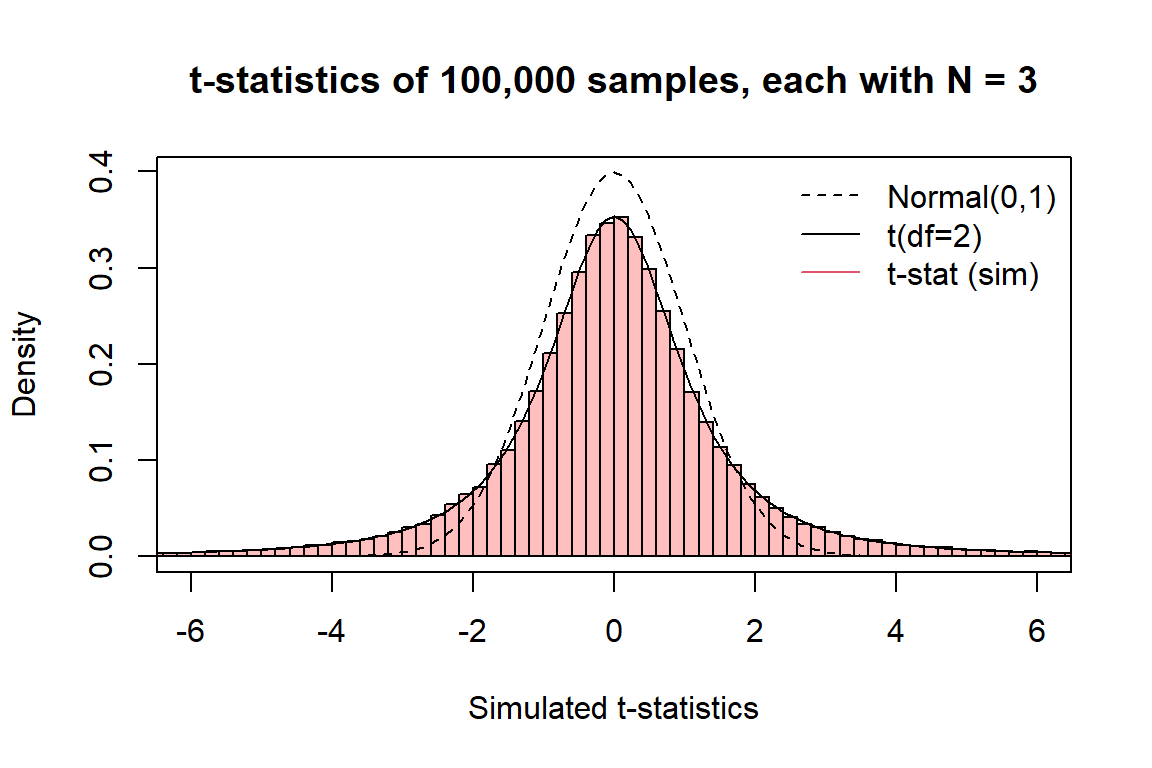
\includegraphics[width=0.7\linewidth,height=0.7\textheight]{_main_files/figure-latex/t-stat-hist-1} 

}

\caption{Histogram of 50,000 t-statistics calculated from 100,000 samples, along with the corresponding theoretical t-distribution (solid line) and a standard normal (dotted line).}\label{fig:t-stat-hist}
\end{figure}

Notice how the histogram and the solid lines are nearly identical? These simulations illustrate that the t-distribution \emph{is} the distribution of t-statistics for a given sample size.

\hypertarget{confidence-intervals}{%
\section{Confidence Intervals}\label{confidence-intervals}}

Say you are interested in knowing the mean of a population (e.g.~barnacle mass on the back beach). You cannot afford to determine the mass of each barnacle, so you take a random sample. You don't know how `good' (i.e.~representative) your sample is. It might have included lots of small barnacles, or big ones, or a wide- or narrow-range of sizes, you can never know (unless you sample everything). When you calculate the mean of this sample you don't know how close it is to the population mean, but you do know the probability associated with that estimate. Confidence intervals capture this uncertainty, and you use the t-distribution to determine them.

We'll invent a population of barnacle diameters, called \texttt{barnacle\_diam}, and then create a histogram of that population and superimpose values on that. Again, these are random numbers so your values will be slightly different from mine.

\begin{Shaded}
\begin{Highlighting}[]
\NormalTok{pop\_size }\OtherTok{\textless{}{-}} \DecValTok{100000}  \CommentTok{\# number of barnacles in the population}
\NormalTok{meta\_mu }\OtherTok{\textless{}{-}} \DecValTok{200}
\NormalTok{meta\_sigma }\OtherTok{\textless{}{-}} \DecValTok{25}
\NormalTok{barnacle\_diam }\OtherTok{\textless{}{-}} \FunctionTok{rnorm}\NormalTok{(pop\_size, }\AttributeTok{mean =}\NormalTok{ meta\_mu, }\AttributeTok{sd =}\NormalTok{ meta\_sigma)}
\NormalTok{mu }\OtherTok{\textless{}{-}} \FunctionTok{mean}\NormalTok{(barnacle\_diam)}
\NormalTok{sigma }\OtherTok{\textless{}{-}} \FunctionTok{sd}\NormalTok{(barnacle\_diam)}
\FunctionTok{hist}\NormalTok{(barnacle\_diam, }\AttributeTok{main =} \ConstantTok{NULL}\NormalTok{)}
\NormalTok{Q95 }\OtherTok{\textless{}{-}} \FunctionTok{quantile}\NormalTok{(barnacle\_diam, }\FunctionTok{c}\NormalTok{(}\FloatTok{0.025}\NormalTok{, }\FloatTok{0.975}\NormalTok{))}
\FunctionTok{abline}\NormalTok{(}\AttributeTok{v =}\NormalTok{ Q95, }\AttributeTok{col =} \StringTok{"green"}\NormalTok{, }\AttributeTok{lwd =} \DecValTok{3}\NormalTok{)}
\FunctionTok{text}\NormalTok{(}\AttributeTok{x=}\NormalTok{Q95[}\DecValTok{2}\NormalTok{], }\AttributeTok{y=}\NormalTok{pop\_size}\SpecialCharTok{/}\DecValTok{7}\NormalTok{, }
     \AttributeTok{labels=}\FunctionTok{paste0}\NormalTok{(}\StringTok{"mu: "}\NormalTok{, }\FunctionTok{round}\NormalTok{(mu, }\DecValTok{1}\NormalTok{), }\StringTok{"}\SpecialCharTok{\textbackslash{}n}\StringTok{sigma:"}\NormalTok{, }\FunctionTok{round}\NormalTok{(sigma, }\DecValTok{1}\NormalTok{)))}
\end{Highlighting}
\end{Shaded}

\begin{figure}

{\centering 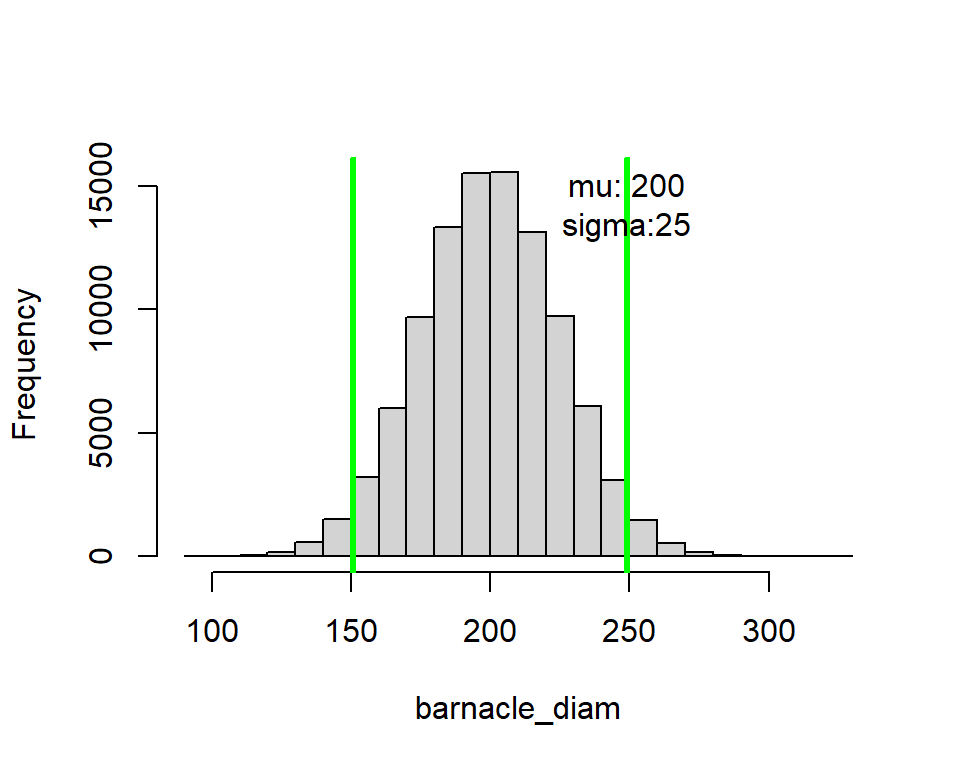
\includegraphics[width=0.5\linewidth,height=0.5\textheight]{_main_files/figure-latex/ci-examp1-1} 

}

\caption{Histogram of a simulated barnacle population with 2.5\% and 97.5\% quantiles.}\label{fig:ci-examp1}
\end{figure}

Now we can take samples from that population: this is the reality, you take samples (usually) from populations where you don't know the true mean and standard deviation. Let's take 4 samples, each with size \texttt{sample\_size}.

\begin{Shaded}
\begin{Highlighting}[]
\FunctionTok{hist}\NormalTok{(barnacle\_diam, }\AttributeTok{main =} \ConstantTok{NULL}\NormalTok{)}
\NormalTok{sample\_size }\OtherTok{\textless{}{-}} \DecValTok{5}
\NormalTok{num\_samples }\OtherTok{\textless{}{-}} \DecValTok{4}
\FunctionTok{abline}\NormalTok{(}\AttributeTok{v =}\NormalTok{ mu, }\AttributeTok{col =} \StringTok{"blue"}\NormalTok{, }\AttributeTok{lwd =} \DecValTok{4}\NormalTok{)}

\ControlFlowTok{for}\NormalTok{ (i }\ControlFlowTok{in} \DecValTok{1}\SpecialCharTok{:}\NormalTok{num\_samples) \{}
\NormalTok{  sample\_i }\OtherTok{\textless{}{-}} \FunctionTok{sample}\NormalTok{(barnacle\_diam, }\AttributeTok{size =}\NormalTok{ sample\_size)}
  \FunctionTok{print}\NormalTok{(sample\_i)}
  \FunctionTok{abline}\NormalTok{(}\AttributeTok{v =} \FunctionTok{mean}\NormalTok{(sample\_i), }\AttributeTok{col =} \StringTok{"red"}\NormalTok{, }\AttributeTok{lwd =} \FloatTok{0.5}\NormalTok{)}
\NormalTok{\}}
\end{Highlighting}
\end{Shaded}

\begin{figure}

{\centering 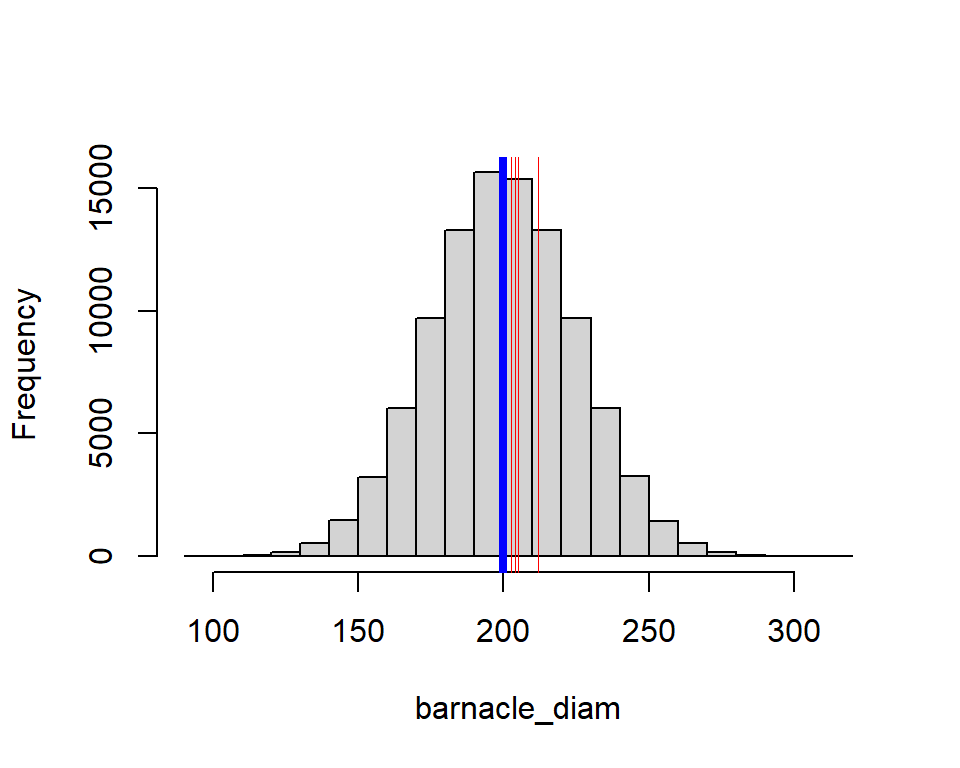
\includegraphics[width=0.5\linewidth,height=0.5\textheight]{_main_files/figure-latex/ci-examp2-1} 

}

\caption{Histogram of the barnacle population showing location of 4 sample means (red lines), each with N = 5. The blue line shows the true population mean mu.}\label{fig:ci-examp2}
\end{figure}

\begin{verbatim}
## [1] 127.0598 204.3132 212.1038 155.2723 202.1684
## [1] 188.9613 173.8530 202.7288 209.3079 203.4615
## [1] 173.6354 170.4280 162.4823 199.2663 203.2909
## [1] 181.7948 218.1346 179.5933 236.8487 204.5922
\end{verbatim}

Our sample means inevitably differ from the true population mean (\(\mu\)), even if only a bit. Likewise, the sample standard deviations will differ from the true population standard deviation (\(\sigma\)). If you keep repeating this sampling you can generate a distribution of sample standard deviations. This distribution is not normal, but is instead related to the chi-square distribution (don't worry too much about this). The point is that if your sample size is small, your estimate of the standard deviation is often very poor.

\begin{Shaded}
\begin{Highlighting}[]
\FunctionTok{par}\NormalTok{(}\AttributeTok{mfrow=}\FunctionTok{c}\NormalTok{(}\DecValTok{2}\NormalTok{,}\DecValTok{2}\NormalTok{))}
\CommentTok{\# sim\_df will hold the sample sizes N, and the median and mean sample sd\textquotesingle{}s }
\NormalTok{num\_samples }\OtherTok{\textless{}{-}} \FloatTok{1e4}
\NormalTok{sim\_df }\OtherTok{\textless{}{-}} \FunctionTok{data.frame}\NormalTok{(}\AttributeTok{N=}\FunctionTok{c}\NormalTok{(}\DecValTok{2}\NormalTok{, }\DecValTok{4}\NormalTok{, }\DecValTok{10}\NormalTok{, }\DecValTok{30}\NormalTok{),}
                     \AttributeTok{sd\_median=}\ConstantTok{NA}\NormalTok{, }\AttributeTok{sd\_mean=}\ConstantTok{NA}\NormalTok{,}
                     \AttributeTok{sd\_q025=}\ConstantTok{NA}\NormalTok{, }\AttributeTok{sd\_q25=}\ConstantTok{NA}\NormalTok{, }\AttributeTok{sd\_q75=}\ConstantTok{NA}\NormalTok{, }\AttributeTok{sd\_q975=}\ConstantTok{NA}\NormalTok{,}
                     \AttributeTok{mn\_median=}\ConstantTok{NA}\NormalTok{, }\AttributeTok{mn\_mean=}\ConstantTok{NA}\NormalTok{,}
                     \AttributeTok{mn\_q025=}\ConstantTok{NA}\NormalTok{, }\AttributeTok{mn\_q25=}\ConstantTok{NA}\NormalTok{, }\AttributeTok{mn\_q75=}\ConstantTok{NA}\NormalTok{, }\AttributeTok{mn\_q975=}\ConstantTok{NA}\NormalTok{) }

\CommentTok{\# for each sample size N, draw a sample and store its mean and sd}
\CommentTok{\# repeat this num\_samples times}
\CommentTok{\# plot a histogram of the sample sd\textquotesingle{}s, then store the mean and median}
\ControlFlowTok{for}\NormalTok{ (i }\ControlFlowTok{in} \DecValTok{1}\SpecialCharTok{:}\FunctionTok{nrow}\NormalTok{(sim\_df)) \{}
\NormalTok{  samp\_sd\_i }\OtherTok{\textless{}{-}} \FunctionTok{numeric}\NormalTok{(num\_samples) }
\NormalTok{  samp\_mn\_i }\OtherTok{\textless{}{-}} \FunctionTok{numeric}\NormalTok{(num\_samples) }
  \ControlFlowTok{for}\NormalTok{ (j }\ControlFlowTok{in} \DecValTok{1}\SpecialCharTok{:}\NormalTok{num\_samples) \{ }
\NormalTok{    sample\_ij }\OtherTok{\textless{}{-}} \FunctionTok{sample}\NormalTok{(barnacle\_diam, }\AttributeTok{size =}\NormalTok{ sim\_df}\SpecialCharTok{$}\NormalTok{N[i])}
\NormalTok{    samp\_sd\_i[j] }\OtherTok{\textless{}{-}} \FunctionTok{sd}\NormalTok{(sample\_ij)}
\NormalTok{    samp\_mn\_i[j] }\OtherTok{\textless{}{-}} \FunctionTok{mean}\NormalTok{(sample\_ij)}
\NormalTok{  \}}
  \FunctionTok{hist}\NormalTok{(samp\_sd\_i, }\AttributeTok{main =} \FunctionTok{paste}\NormalTok{(num\_samples, }\StringTok{"sample SDs for N ="}\NormalTok{, sim\_df}\SpecialCharTok{$}\NormalTok{N[i]), }
       \AttributeTok{breaks =} \DecValTok{20}\NormalTok{, }\AttributeTok{xlim =} \FunctionTok{c}\NormalTok{(}\DecValTok{0}\NormalTok{, }\DecValTok{100}\NormalTok{))}
  \FunctionTok{abline}\NormalTok{(}\AttributeTok{v =}\NormalTok{ sigma, }\AttributeTok{col =} \StringTok{"blue"}\NormalTok{, }\AttributeTok{lwd =} \DecValTok{2}\NormalTok{)}
\NormalTok{  sim\_df[i, }\DecValTok{2}\SpecialCharTok{:}\DecValTok{13}\NormalTok{] }\OtherTok{\textless{}{-}} \FunctionTok{c}\NormalTok{(}\FunctionTok{median}\NormalTok{(samp\_sd\_i), }\FunctionTok{mean}\NormalTok{(samp\_sd\_i),}
                       \FunctionTok{quantile}\NormalTok{(samp\_sd\_i, }\AttributeTok{probs =} \FunctionTok{c}\NormalTok{(}\FloatTok{0.025}\NormalTok{, }\FloatTok{0.25}\NormalTok{, }\FloatTok{0.75}\NormalTok{, }\FloatTok{0.975}\NormalTok{)),}
                       \FunctionTok{median}\NormalTok{(samp\_mn\_i), }\FunctionTok{mean}\NormalTok{(samp\_mn\_i),}
                       \FunctionTok{quantile}\NormalTok{(samp\_mn\_i, }\AttributeTok{probs =} \FunctionTok{c}\NormalTok{(}\FloatTok{0.025}\NormalTok{, }\FloatTok{0.25}\NormalTok{, }\FloatTok{0.75}\NormalTok{, }\FloatTok{0.975}\NormalTok{)))}
\NormalTok{\}}
\end{Highlighting}
\end{Shaded}

\begin{figure}

{\centering 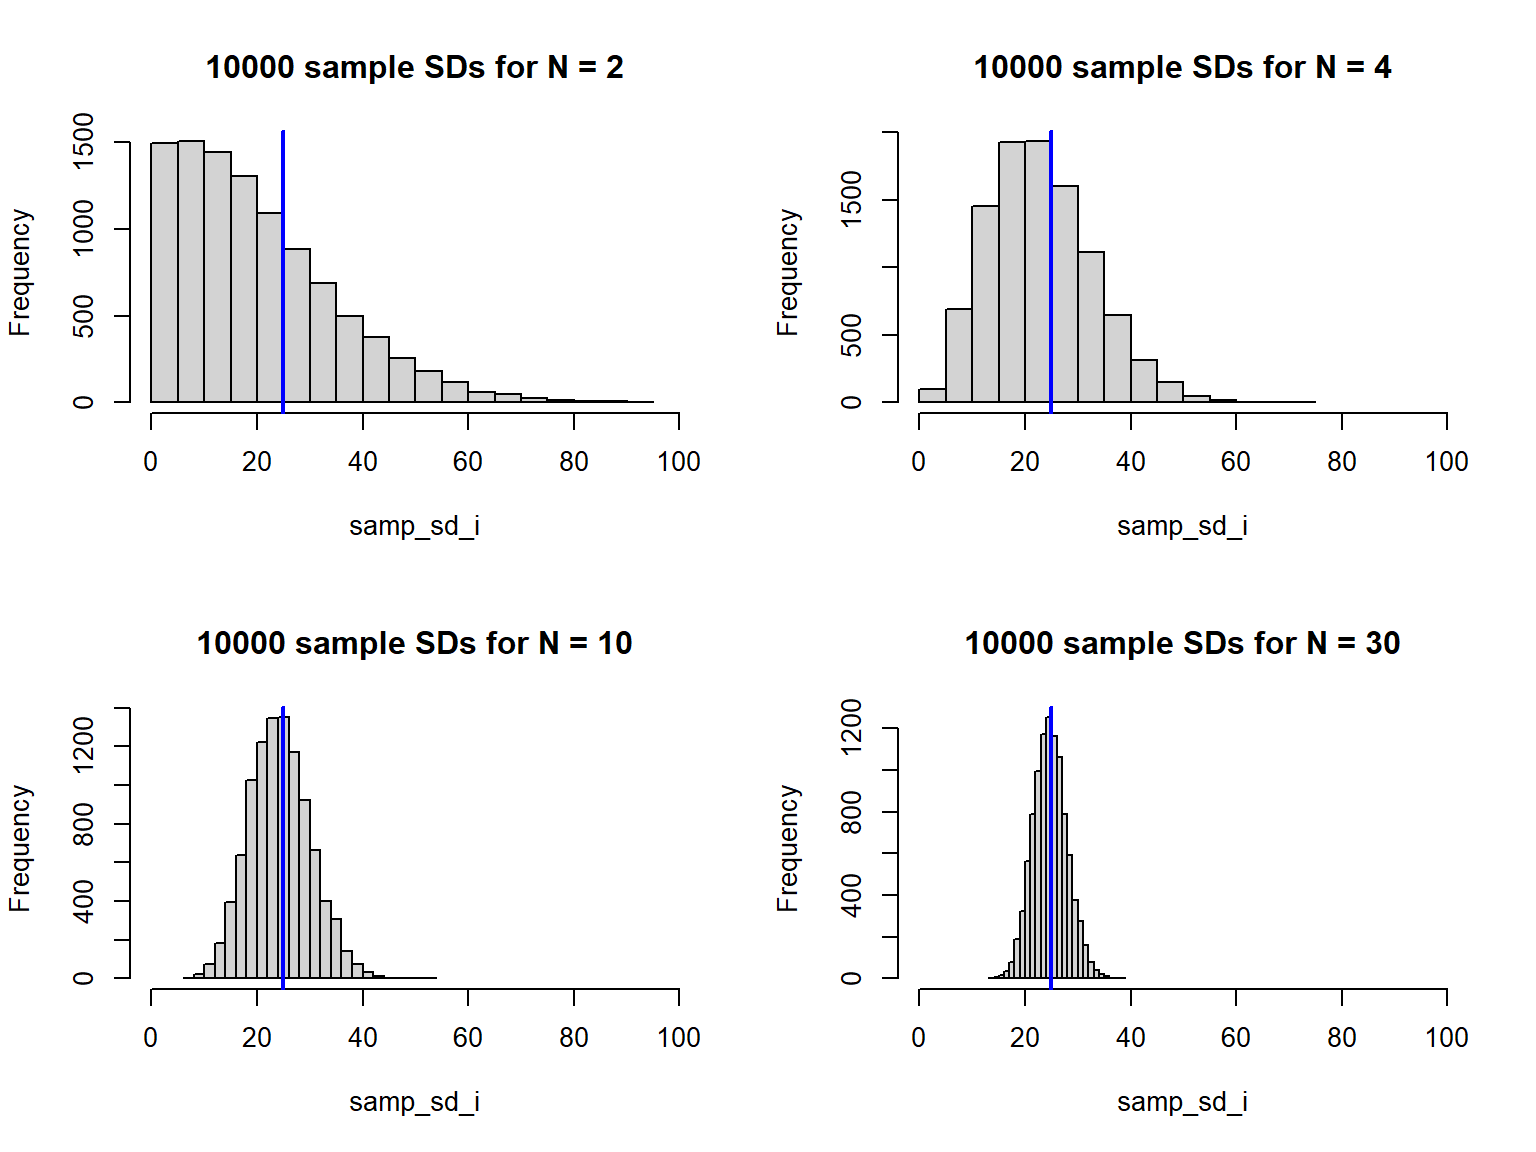
\includegraphics[width=0.7\linewidth,height=0.7\textheight]{_main_files/figure-latex/sd-N-hist-1} 

}

\caption{Histograms of sample standard deviations from repeated samples of the same population. The true population standard deviation is shown in blue.}\label{fig:sd-N-hist}
\end{figure}

\begin{Shaded}
\begin{Highlighting}[]
\FunctionTok{par}\NormalTok{(}\AttributeTok{mfrow=}\FunctionTok{c}\NormalTok{(}\DecValTok{1}\NormalTok{,}\DecValTok{2}\NormalTok{))}
\FunctionTok{plot}\NormalTok{(sim\_df}\SpecialCharTok{$}\NormalTok{N, sim\_df}\SpecialCharTok{$}\NormalTok{sd\_median,}
  \AttributeTok{xlim =} \FunctionTok{c}\NormalTok{(}\DecValTok{0}\NormalTok{, }\DecValTok{30}\NormalTok{), }\AttributeTok{ylim =} \FunctionTok{range}\NormalTok{(}\FunctionTok{c}\NormalTok{(sim\_df[,}\DecValTok{2}\SpecialCharTok{:}\DecValTok{7}\NormalTok{], sigma)),}
  \AttributeTok{type =} \StringTok{"b"}\NormalTok{, }\AttributeTok{xlab =} \StringTok{"Sample size"}\NormalTok{, }\AttributeTok{ylab =} \StringTok{"Standard deviation"}
\NormalTok{)}
\FunctionTok{segments}\NormalTok{(sim\_df}\SpecialCharTok{$}\NormalTok{N, sim\_df}\SpecialCharTok{$}\NormalTok{sd\_q25, sim\_df}\SpecialCharTok{$}\NormalTok{N, sim\_df}\SpecialCharTok{$}\NormalTok{sd\_q75, }\AttributeTok{lwd=}\DecValTok{2}\NormalTok{)}
\FunctionTok{segments}\NormalTok{(sim\_df}\SpecialCharTok{$}\NormalTok{N, sim\_df}\SpecialCharTok{$}\NormalTok{sd\_q025, sim\_df}\SpecialCharTok{$}\NormalTok{N, sim\_df}\SpecialCharTok{$}\NormalTok{sd\_q975)}
\FunctionTok{lines}\NormalTok{(sim\_df}\SpecialCharTok{$}\NormalTok{N, sim\_df}\SpecialCharTok{$}\NormalTok{sd\_mean, }\AttributeTok{type =} \StringTok{"b"}\NormalTok{, }\AttributeTok{col =} \StringTok{"dodgerblue"}\NormalTok{)}
\FunctionTok{abline}\NormalTok{(}\AttributeTok{h =}\NormalTok{ sigma, }\AttributeTok{lty =} \DecValTok{2}\NormalTok{)}
\FunctionTok{legend}\NormalTok{(}\StringTok{"topright"}\NormalTok{, }\FunctionTok{c}\NormalTok{(}\StringTok{"Mean sample SD"}\NormalTok{, }\StringTok{"Median sample SD"}\NormalTok{, }\StringTok{"True SD"}\NormalTok{),}
  \AttributeTok{col =} \FunctionTok{c}\NormalTok{(}\StringTok{"black"}\NormalTok{, }\StringTok{"dodgerblue"}\NormalTok{, }\StringTok{"black"}\NormalTok{),}
  \AttributeTok{lty =} \FunctionTok{c}\NormalTok{(}\DecValTok{1}\NormalTok{, }\DecValTok{1}\NormalTok{, }\DecValTok{2}\NormalTok{), }\AttributeTok{pch =} \FunctionTok{c}\NormalTok{(}\DecValTok{1}\NormalTok{, }\DecValTok{1}\NormalTok{, }\ConstantTok{NA}\NormalTok{), }\AttributeTok{bty =} \StringTok{"n"}
\NormalTok{)}
\FunctionTok{plot}\NormalTok{(sim\_df}\SpecialCharTok{$}\NormalTok{N, sim\_df}\SpecialCharTok{$}\NormalTok{mn\_median,}
  \AttributeTok{xlim =} \FunctionTok{c}\NormalTok{(}\DecValTok{0}\NormalTok{, }\DecValTok{30}\NormalTok{), }\AttributeTok{ylim =} \FunctionTok{range}\NormalTok{(}\FunctionTok{c}\NormalTok{(sim\_df[,}\DecValTok{8}\SpecialCharTok{:}\DecValTok{13}\NormalTok{], mu)),}
  \AttributeTok{type =} \StringTok{"b"}\NormalTok{, }\AttributeTok{xlab =} \StringTok{"Sample size"}\NormalTok{, }\AttributeTok{ylab =} \StringTok{"Mean"}
\NormalTok{)}
\FunctionTok{segments}\NormalTok{(sim\_df}\SpecialCharTok{$}\NormalTok{N, sim\_df}\SpecialCharTok{$}\NormalTok{mn\_q25, sim\_df}\SpecialCharTok{$}\NormalTok{N, sim\_df}\SpecialCharTok{$}\NormalTok{mn\_q75, }\AttributeTok{lwd=}\DecValTok{2}\NormalTok{)}
\FunctionTok{segments}\NormalTok{(sim\_df}\SpecialCharTok{$}\NormalTok{N, sim\_df}\SpecialCharTok{$}\NormalTok{mn\_q025, sim\_df}\SpecialCharTok{$}\NormalTok{N, sim\_df}\SpecialCharTok{$}\NormalTok{mn\_q975)}
\FunctionTok{lines}\NormalTok{(sim\_df}\SpecialCharTok{$}\NormalTok{N, sim\_df}\SpecialCharTok{$}\NormalTok{mn\_mean, }\AttributeTok{type =} \StringTok{"b"}\NormalTok{, }\AttributeTok{col =} \StringTok{"dodgerblue"}\NormalTok{)}
\FunctionTok{abline}\NormalTok{(}\AttributeTok{h =}\NormalTok{ mu, }\AttributeTok{lty =} \DecValTok{2}\NormalTok{)}
\FunctionTok{legend}\NormalTok{(}\StringTok{"topright"}\NormalTok{, }\FunctionTok{c}\NormalTok{(}\StringTok{"Mean sample mean"}\NormalTok{, }\StringTok{"Median sample mean"}\NormalTok{, }\StringTok{"True mean"}\NormalTok{),}
  \AttributeTok{col =} \FunctionTok{c}\NormalTok{(}\StringTok{"black"}\NormalTok{, }\StringTok{"dodgerblue"}\NormalTok{, }\StringTok{"black"}\NormalTok{),}
  \AttributeTok{lty =} \FunctionTok{c}\NormalTok{(}\DecValTok{1}\NormalTok{, }\DecValTok{1}\NormalTok{, }\DecValTok{2}\NormalTok{), }\AttributeTok{pch =} \FunctionTok{c}\NormalTok{(}\DecValTok{1}\NormalTok{, }\DecValTok{1}\NormalTok{, }\ConstantTok{NA}\NormalTok{), }\AttributeTok{bty =} \StringTok{"n"}
\NormalTok{)}
\end{Highlighting}
\end{Shaded}

\begin{figure}

{\centering 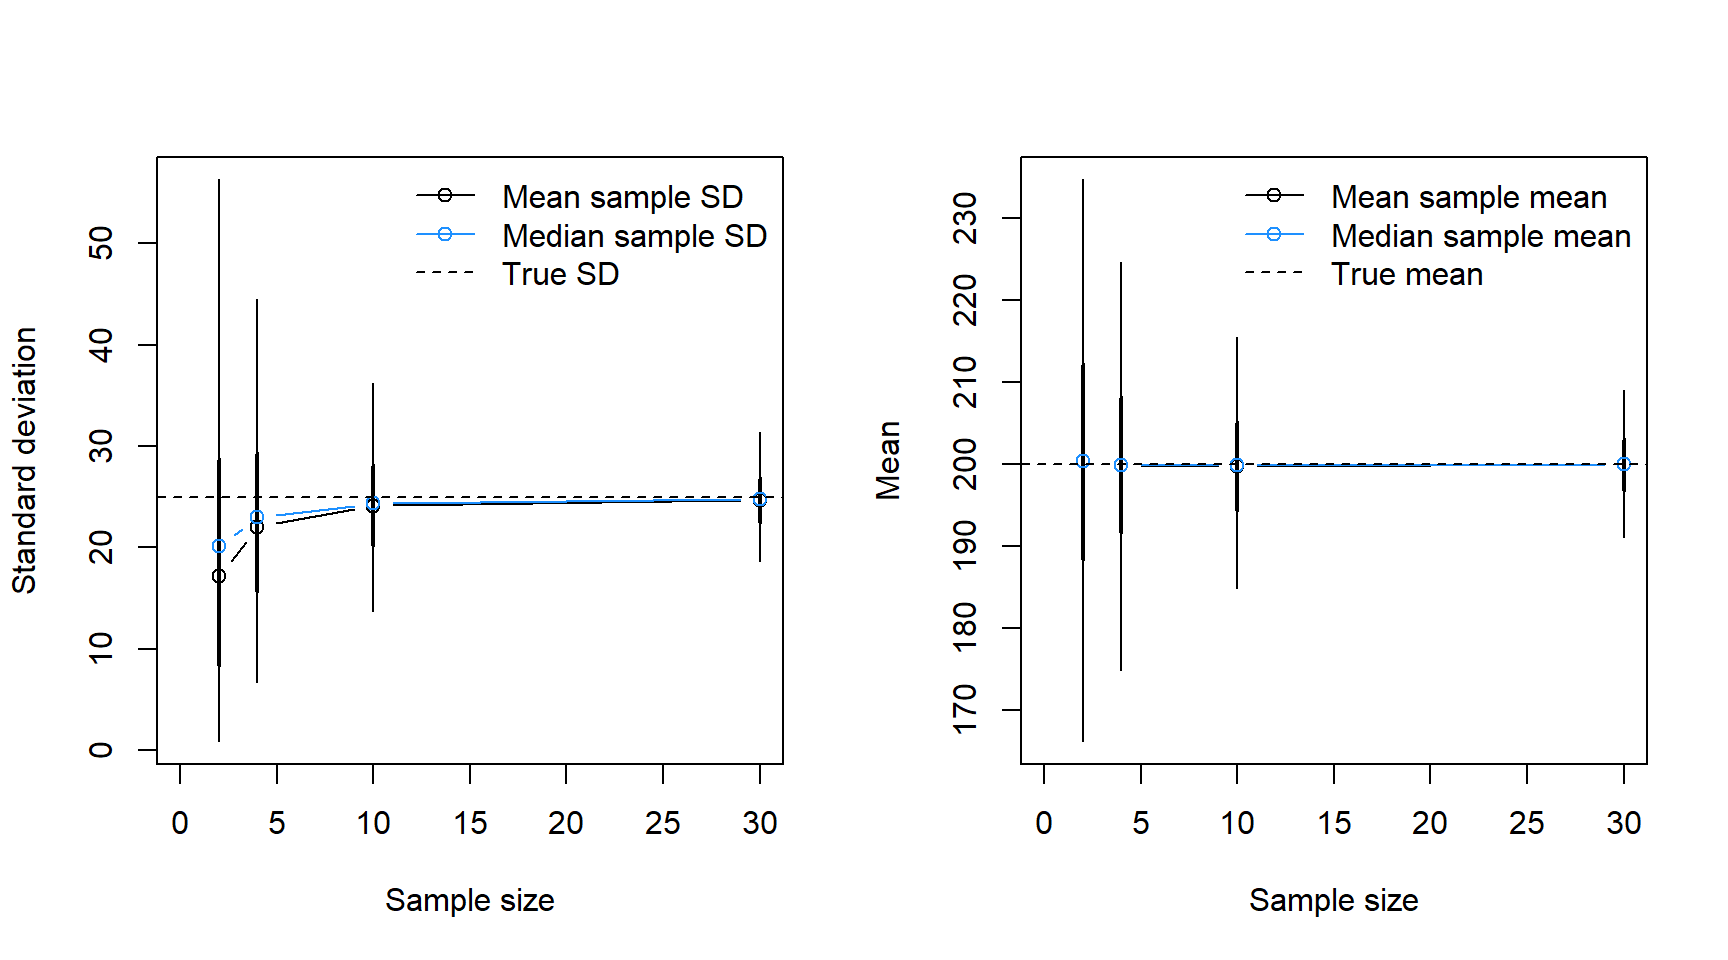
\includegraphics[width=0.7\linewidth,height=0.7\textheight]{_main_files/figure-latex/sd-N-lines-1} 

}

\caption{Mean (black), median (blue), and 50\% and 95\% quantiles (vertical lines) for (left) sample standard deviations at each sample size compared to the true population standard deviation (dotted line) or for the (right) sample means.}\label{fig:sd-N-lines}
\end{figure}

\emph{Q133. What is the most common standard deviation for your samples by sample size?}

The t-distribution allows for the fact that the standard deviation of small samples is, usually, less than that of the population as seen in Fig. \ref{fig:sd-N-hist}.

The take home message here is that when you take a sample from a population with unknown \(\mu\) and \(\sigma\), you won't know how `accurate' you sample is but you do know how your random samples `behave' - they are modelled using the t-distribution. From this knowledge you can build a 95\% confidence interval which is described as an interval which, if repeated for 100 samples, would include \(\mu\) within its boundaries in 95 of those samples (on average). Read that again. You don't have knowledge of the true value of the mean or sd (as you did for Z score calucations) and the t-distribution accounts for this uncertainty.

\begin{Shaded}
\begin{Highlighting}[]
\NormalTok{num\_samples }\OtherTok{\textless{}{-}} \DecValTok{5}
\NormalTok{sample\_size }\OtherTok{\textless{}{-}} \DecValTok{3}

\CommentTok{\# plot population}
\FunctionTok{hist}\NormalTok{(barnacle\_diam, }\AttributeTok{xlim =} \FunctionTok{c}\NormalTok{(mu}\DecValTok{{-}6}\SpecialCharTok{*}\NormalTok{sigma, mu}\SpecialCharTok{+}\DecValTok{6}\SpecialCharTok{*}\NormalTok{sigma), }
     \AttributeTok{main =} \ConstantTok{NULL}\NormalTok{, }\AttributeTok{ylim =} \FunctionTok{c}\NormalTok{(}\DecValTok{0}\NormalTok{, }\FunctionTok{length}\NormalTok{(barnacle\_diam)}\SpecialCharTok{/}\DecValTok{6}\NormalTok{),}
     \AttributeTok{col =} \StringTok{"grey90"}\NormalTok{, }\AttributeTok{border =} \StringTok{"grey50"}\NormalTok{, }\AttributeTok{xlab =} \StringTok{"Barnacle diameter"}\NormalTok{)}
\FunctionTok{abline}\NormalTok{(}\AttributeTok{v =}\NormalTok{ mu, }\AttributeTok{col =} \StringTok{"blue"}\NormalTok{, }\AttributeTok{lwd =} \DecValTok{2}\NormalTok{)}
\NormalTok{y\_pos }\OtherTok{\textless{}{-}} \FunctionTok{seq}\NormalTok{(}\DecValTok{0}\NormalTok{, }\FunctionTok{length}\NormalTok{(barnacle\_diam)}\SpecialCharTok{/}\DecValTok{6}\NormalTok{, }\AttributeTok{length.out=}\NormalTok{num\_samples)}

\CommentTok{\# draw samples, calculate mean and 95\% CIs, and plot them}
\ControlFlowTok{for}\NormalTok{ (i }\ControlFlowTok{in} \DecValTok{1}\SpecialCharTok{:}\NormalTok{num\_samples) \{}
\NormalTok{  sample\_i }\OtherTok{\textless{}{-}} \FunctionTok{sample}\NormalTok{(barnacle\_diam, }\AttributeTok{size =}\NormalTok{ sample\_size)}
  \FunctionTok{points}\NormalTok{(}\AttributeTok{x =} \FunctionTok{mean}\NormalTok{(sample\_i), }\AttributeTok{y =}\NormalTok{ y\_pos[i], }\AttributeTok{col =} \StringTok{"red"}\NormalTok{, }\AttributeTok{pch =} \DecValTok{16}\NormalTok{, }\AttributeTok{cex =} \FloatTok{0.75}\NormalTok{)}
\NormalTok{  sample\_ci }\OtherTok{\textless{}{-}} \FunctionTok{c}\NormalTok{(}
    \FunctionTok{mean}\NormalTok{(sample\_i) }\SpecialCharTok{+} \FunctionTok{qt}\NormalTok{(}\FloatTok{0.025}\NormalTok{, (sample\_size }\SpecialCharTok{{-}} \DecValTok{1}\NormalTok{)) }\SpecialCharTok{*}\NormalTok{ (}\FunctionTok{sd}\NormalTok{(sample\_i) }\SpecialCharTok{/}\NormalTok{ sample\_size}\SpecialCharTok{\^{}}\FloatTok{0.5}\NormalTok{),}
    \FunctionTok{mean}\NormalTok{(sample\_i) }\SpecialCharTok{+} \FunctionTok{qt}\NormalTok{(}\FloatTok{0.975}\NormalTok{, (sample\_size }\SpecialCharTok{{-}} \DecValTok{1}\NormalTok{)) }\SpecialCharTok{*}\NormalTok{ (}\FunctionTok{sd}\NormalTok{(sample\_i) }\SpecialCharTok{/}\NormalTok{ sample\_size}\SpecialCharTok{\^{}}\FloatTok{0.5}\NormalTok{)}
\NormalTok{  )}
  \FunctionTok{arrows}\NormalTok{(sample\_ci[}\DecValTok{1}\NormalTok{], y\_pos[i], sample\_ci[}\DecValTok{2}\NormalTok{], y\_pos[i], }
         \AttributeTok{col =} \StringTok{"red"}\NormalTok{, }\AttributeTok{code =} \DecValTok{3}\NormalTok{, }\AttributeTok{angle =} \DecValTok{90}\NormalTok{, }\AttributeTok{length=}\FloatTok{0.05}\NormalTok{)}
\NormalTok{\}}
\end{Highlighting}
\end{Shaded}

\begin{figure}

{\centering 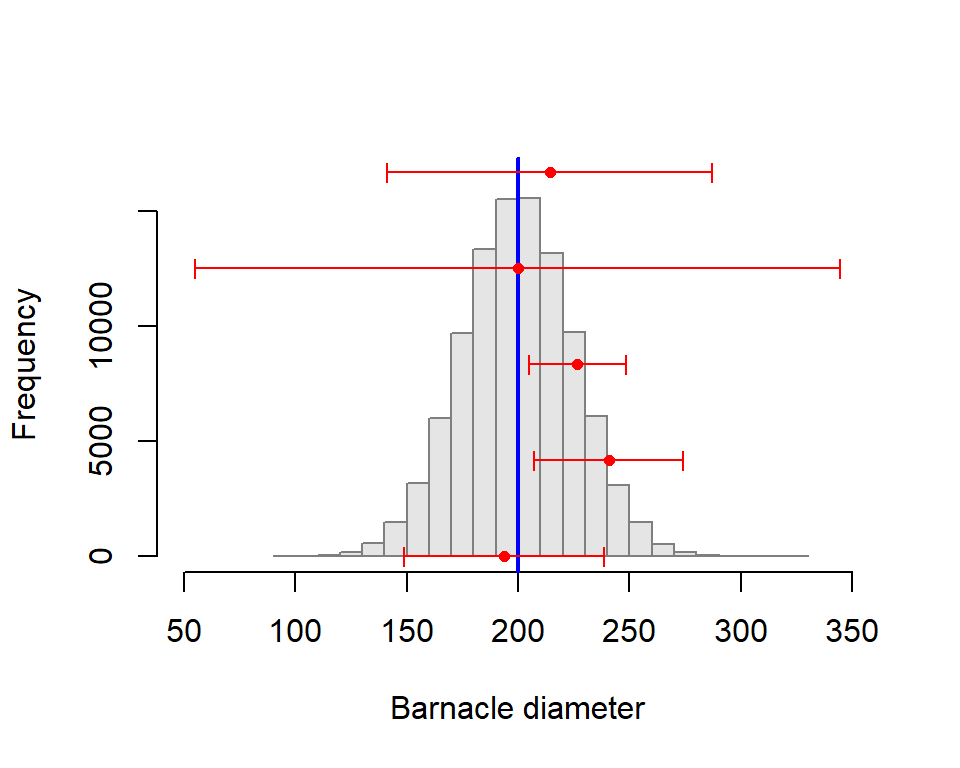
\includegraphics[width=0.5\linewidth,height=0.5\textheight]{_main_files/figure-latex/ci-examp3-1} 

}

\caption{Histogram illustrating the barnacle population with population mean (blue) and sample means with 95\% CIs (red) repeated across 20 samples.}\label{fig:ci-examp3}
\end{figure}

\emph{Q134. Try different values for \texttt{sample\_size}. How does this influence the width of your CIs?}

\emph{Q135. What proportion of your 95\% CIs would you expect to include the true value of the mean? Does the sample size have an impact on this?}

\emph{Q136. Keep repeating the above code until you get an example where your 95\% CI misses the true value of the mean.}

\emph{Q137. See if you can find the relevant bit of the code, and determine 99\% and 90\% or 75\% CIs (pick any value you fancy, but note that some values are likely to put the CIs some distance from the mean so get ready to adjust your axis limits which are set to 6} \(\sigma\) \emph{on either side of} \(\mu\)\emph{).}

Let's explore the influence of sample size on the width of the confidence interval a little more.

We will plot the resultant mean estimate and 95\% CI on Fig. \ref{fig:ci-v-N}. NOTE: the example shown in Fig. \ref{fig:ci-v-N} is a random example, not linked to the output below. Repeat this process, but this time determine the mean and sd (or variance) for samples of 2, 5 and 10. Do this simply by changing \texttt{n=…} in \texttt{rnorm()} Repeat this 5 times for each sample size and sketch your results (where they fit) onto Fig. \ref{fig:ci-v-N}.

\begin{Shaded}
\begin{Highlighting}[]
\NormalTok{a }\OtherTok{\textless{}{-}} \FunctionTok{rnorm}\NormalTok{(}\AttributeTok{n =} \DecValTok{10}\NormalTok{, }\AttributeTok{mean =} \DecValTok{100}\NormalTok{, }\AttributeTok{sd =} \DecValTok{10}\NormalTok{)}
\FunctionTok{signif}\NormalTok{(a, }\DecValTok{3}\NormalTok{)}
\end{Highlighting}
\end{Shaded}

\begin{verbatim}
##  [1]  97.9 102.0  78.1  93.2 102.0 110.0  94.1 102.0  98.4 102.0
\end{verbatim}

\begin{Shaded}
\begin{Highlighting}[]
\FunctionTok{t.test}\NormalTok{(a, }\AttributeTok{mu =} \DecValTok{100}\NormalTok{)}
\end{Highlighting}
\end{Shaded}

\begin{verbatim}
## 
##  One Sample t-test
## 
## data:  a
## t = -0.77679, df = 9, p-value = 0.4572
## alternative hypothesis: true mean is not equal to 100
## 95 percent confidence interval:
##   91.89388 103.96207
## sample estimates:
## mean of x 
##  97.92798
\end{verbatim}

\begin{figure}

{\centering 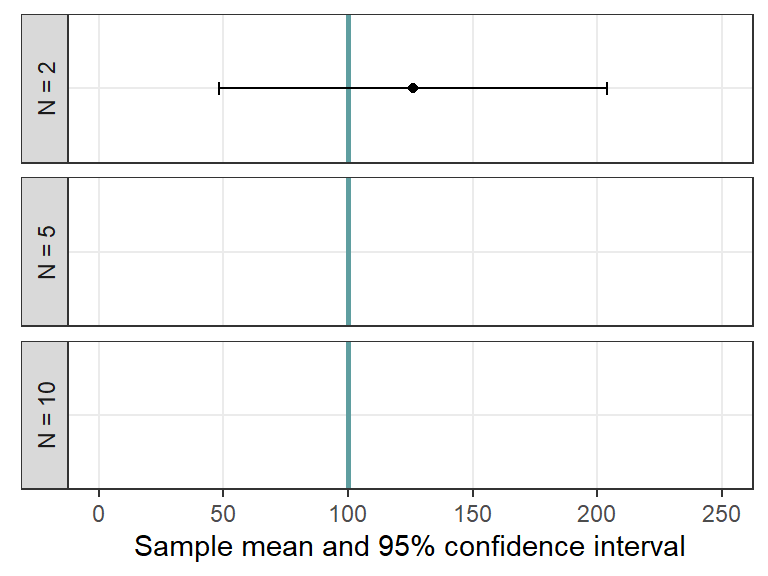
\includegraphics[width=0.6\linewidth,height=0.6\textheight]{_main_files/figure-latex/ci-v-N-1} 

}

\caption{Confidence interval size vs. sample size.}\label{fig:ci-v-N}
\end{figure}

\emph{Q138. Look at your 95\% confidence intervals -- are they getting broader or narrower as your sample size decreases?}

\emph{Q139. What proportion of 95\% CIs would you expect to include the true value of the mean?}

\hypertarget{comparing-means-two-sample-t-tests}{%
\section{Comparing means (two-sample t tests)}\label{comparing-means-two-sample-t-tests}}

The two-sample t-test is one of the most widely used inferential statistical tests. The two-sample t-test is a special case of analysis of variance (ANOVA) where you are only comparing two means. The results are identical and so we do not focus on two-sample t-tests. You need to know of the existence of the two-sample t-test because it is so commonly used and cited, but you will be comparing means using ANOVA in Practical \ref{glm}.

\hypertarget{non-parametric-tests}{%
\section{Non-parametric Tests}\label{non-parametric-tests}}

Non-parametric tests are often used to compare samples where the data are non-continuous or fail the assumptions of parametric general linear models, typically converting data to ranks rather than using the actual values. Non-parametric test include `classics' such as the `Mood' and `Wilcoxon' tests. However, we make you aware of the GLM family which will usually supply you with a much more elegant solution to model data that doesn't fit the simple linear model. You should be aware of the existence of `non-parametric' tests because they are prevalent in the literature. Remind yourself of the disadvantages of non-parametric tests.

\hypertarget{conclusions-3}{%
\section{Conclusions}\label{conclusions-3}}

The t-test is a `classic' statistical test which doesn't assume knowledge of population parameters. The strength of the t-test (its ability to quantify differences between samples) is proportional to the sample size. The larger the sample size, the better the estimate of the population parameters and the more precisely we are to be able to detect differences between the means.

The central limit theorem tells us that the means of non-normally distributed data will be normally distributed if the sample size is sufficiently large. If your sample size is \(>\) 30 it is likely that the means of that sample will be normally distributed regardless of the distribution of the original data.

Parametric tests including the t-test are quite `robust' against deviations from normality, particularly as sample sizes increase. However, parametric test are less robust against heteroscedasticity, regardless of sample size. Always check this assumption and be prepared to transform the data if the assumption of homoscedasticity is not tenable (more of this in Practical \ref{glm}).

The t-test is in the `general linear model' family (and this is a subset of the generalised linear modelling family). General linear models are usually used to model continuous data. If you have count data, you should start with a different member of the GLM family (you might not be able to transform count data to something approximating a normal distribution). Non-parametric tests are frequently adopted when data do not conform to the assumptions of normality but they are invariably used for NHST with all the inherent problems with that approach.

A final reminder with regard to many statistical tests, including all in the GLM family: they make the assumption that data are independent. You must always ensure that your experimental design lends itself to making independent observations IN RELATION TO THE QUESTION YOU ARE ASKING. This is the most critical and fundamental of the assumptions of parametric and non-parametric tests. Non-independence (e.g.~measuring the same `subject' (e.g.~an urchin) over time) can be modelled using more complex `mixed' models. Application of mixed modelling is beyond this course but you should be aware of the limitations of the techniques that you are learning and know where to go next.

\hypertarget{glm}{%
\chapter{General Linear Models}\label{glm}}

General linear models are a key member of the generalised linear modelling family and they are among the most widely used and reported models in the marine science literature, particularly biology. This course focuses on two subsets of linear models: ANOVA and regression. ANOVA and regression are typically used for different data modelling scenarios: ANOVA when you've got a categorical predictor variable(s) and regression when your predictor is continuous.

\hypertarget{analysis-of-variance-anova}{%
\section{Analysis of variance (ANOVA)}\label{analysis-of-variance-anova}}

ANOVA is a widely used modelling approach that enables you to compare means and put confidence intervals on the differences between those means. For a predictor with only two categories, ANOVA is identical to the 2-sample t-test, so we'll just use ANOVA.

When you see ``analysis of variance'', think ``analysis of means''. In an ANOVA, we analyse the variance in the data in order to compare the means of different groups. In an ANOVA, we compare means by determining the ratio of {[}the variance between treatments and the overall mean (large black arrows in Fig. \ref{fig:var-sources}){]} and {[}the variance within treatments (sum of the dotted arrows in Fig. \ref{fig:var-sources}){]}. The black line under the red dots in Fig. \ref{fig:var-sources} shows the actual data distribution and the actual parameters for mean values (50 and 150 cm for A and B respectively). You then take samples from A and B (n=4 in this example) and, from these, derive your parameter estimates for the mean of each group and the overall mean.

In Fig. \ref{fig:var-sources} below you can see that the solid black arrows are much larger than the dotted ones leading you to think that the chance that these two samples are drawn from the same population (with a value of the overall mean) as very unlikely. Make sure you understand Fig. \ref{fig:var-sources} (more detail in the ANOVA lecture).

In most circumstances you know that the means that you are comparing with ANOVA are different (i.e.~that testing a null hypothesis of no difference isn't useful). ANOVA allows you to put confidence intervals around differences between means, or groups of means.

\begin{figure}
\centerline{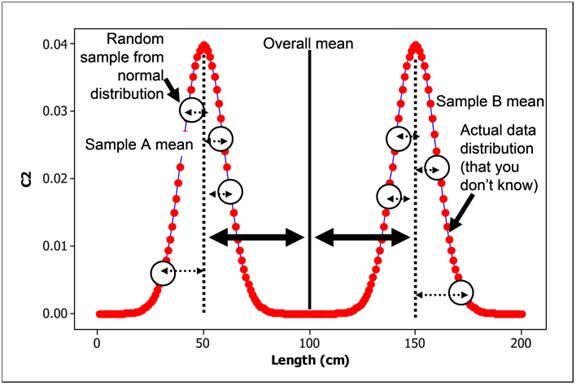
\includegraphics[width=0.6\textwidth]{figs/ANOVA_sources_of_var.png}}
\caption{Sources of variation (within group and between groups) as quantified by ANOVA.}
\label{fig:var-sources}
\end{figure}

\hypertarget{anova-in-r}{%
\subsection{ANOVA in R}\label{anova-in-r}}

There are numerous variations on the theme of ANOVA. We cover one-way ANOVA and we mention two-way ANOVA with and without replication. The objective of ANOVA is to establish the size of the difference (called the `effect size') between different groups (e.g., treatments or locations) and put a confidence interval on those differences.

\hypertarget{one-way-anova}{%
\subsection{One-way ANOVA}\label{one-way-anova}}

One-way ANOVA is a procedure we use to estimate the magnitude of differences between means of \(\geq\) 2 groups. We also use it to put confidence intervals on those differences.

The first example data is the yield in \(\mu g\) C \(ml^{-1}\) of a species of microalgae (\emph{Isochrysis galbana}) in laboratory culture exposed to three light levels (low, medium and high). We are interested in these particular light levels because they represent the means of winter, spring, and summer Scottish sun intensity. The data are in worksheet `Microalgae'.

Note: the function to conduct an ANOVA is \texttt{aov()}. The function \texttt{anova()} converts various statistical model outputs to the standard ANOVA-table output (including any from the GLM family).

\begin{Shaded}
\begin{Highlighting}[]
\FunctionTok{library}\NormalTok{(readxl)}
\NormalTok{algae\_wide\_df }\OtherTok{\textless{}{-}} \FunctionTok{read\_excel}\NormalTok{(}\StringTok{"data/practical\_5.xlsx"}\NormalTok{, }\AttributeTok{sheet =} \StringTok{"Microalgae"}\NormalTok{)}
\CommentTok{\# check these data as usual}
\end{Highlighting}
\end{Shaded}

\emph{Q158. What is your objective in this type of experiment? What are you interested in estimating?}

\emph{Q159. What assumptions should be met prior to undertaking parametric ANOVA?}

\emph{Q160. Under which circumstances could you begin to relax the assumption that the data are normally distributed (think central limit theorem)?}

\emph{Q161. Given your sample size can we assume normality of means?}

\emph{Q162. Are the data normally distributed (be careful how you word your answer to this question, see the following question)?}

\emph{Q163. Is it reasonable to assume that these data are drawn from a population that is normally distributed?}

We can check the homoscedasticity assumption using Bartlett's test. Before we can use this test we need to rearrange the data so that the data is in a single indexed column. We'll use the \emph{tidyverse} as before.

\begin{Shaded}
\begin{Highlighting}[]
\FunctionTok{library}\NormalTok{(tidyverse)}
\FunctionTok{head}\NormalTok{(algae\_wide\_df, }\DecValTok{2}\NormalTok{)}
\end{Highlighting}
\end{Shaded}

\begin{verbatim}
## # A tibble: 2 x 3
##     low medium  high
##   <dbl>  <dbl> <dbl>
## 1  13.1   12    14.2
## 2  11.5   11.5  13.1
\end{verbatim}

\begin{Shaded}
\begin{Highlighting}[]
\NormalTok{algae\_df }\OtherTok{\textless{}{-}}\NormalTok{ algae\_wide\_df }\SpecialCharTok{|\textgreater{}}
  \FunctionTok{pivot\_longer}\NormalTok{(}\FunctionTok{everything}\NormalTok{(), }\AttributeTok{names\_to =} \StringTok{"Treatment"}\NormalTok{, }\AttributeTok{values\_to =} \StringTok{"Yield"}\NormalTok{)}
\FunctionTok{glimpse}\NormalTok{(algae\_df, }\AttributeTok{width=}\DecValTok{80}\NormalTok{)}
\end{Highlighting}
\end{Shaded}

\begin{verbatim}
## Rows: 15
## Columns: 2
## $ Treatment <chr> "low", "medium", "high", "low", "medium", "high", "low", "me~
## $ Yield     <dbl> 13.07599, 12.00000, 14.20000, 11.53923, 11.50000, 13.10000, ~
\end{verbatim}

\begin{Shaded}
\begin{Highlighting}[]
\FunctionTok{bartlett.test}\NormalTok{(Yield }\SpecialCharTok{\textasciitilde{}}\NormalTok{ Treatment, }\AttributeTok{data =}\NormalTok{ algae\_df) }\CommentTok{\#?bartlett.test}
\end{Highlighting}
\end{Shaded}

\begin{verbatim}
## 
##  Bartlett test of homogeneity of variances
## 
## data:  Yield by Treatment
## Bartlett's K-squared = 2.8413, df = 2, p-value = 0.2416
\end{verbatim}

\emph{Q164. With regard to Bartlett's test, is the assumption of homogeneity reasonable?}

A more elegant (and much better) way of checking model assumptions is to check residual patterns. A `residual' is the difference between an actual data value and that predicted by the model. Here we have randomly assigned five cultures each of the same species to three specific treatments (light levels).

\emph{Q165. What type of experiment is this (how many factors, are they fixed or random)?}

Next to conduct the analysis:

\begin{Shaded}
\begin{Highlighting}[]
\NormalTok{algae\_aov }\OtherTok{\textless{}{-}} \FunctionTok{aov}\NormalTok{(Yield }\SpecialCharTok{\textasciitilde{}}\NormalTok{ Treatment, }\AttributeTok{data =}\NormalTok{ algae\_df) }\CommentTok{\# ?aov}
\end{Highlighting}
\end{Shaded}

Before we look at the output, let's assess the assumptions using the residuals. The default residual plots created by R are shown in Fig. \ref{fig:algae-aov} and enables us to rapidly assess whether the model assumptions are reasonable.

\begin{Shaded}
\begin{Highlighting}[]
\FunctionTok{par}\NormalTok{(}\AttributeTok{mfrow =} \FunctionTok{c}\NormalTok{(}\DecValTok{2}\NormalTok{, }\DecValTok{2}\NormalTok{), }\AttributeTok{mar=}\FunctionTok{c}\NormalTok{(}\DecValTok{4}\NormalTok{,}\DecValTok{4}\NormalTok{,}\DecValTok{1}\NormalTok{,}\DecValTok{1}\NormalTok{)) }
\FunctionTok{plot}\NormalTok{(algae\_aov) }
\end{Highlighting}
\end{Shaded}

\begin{figure}

{\centering 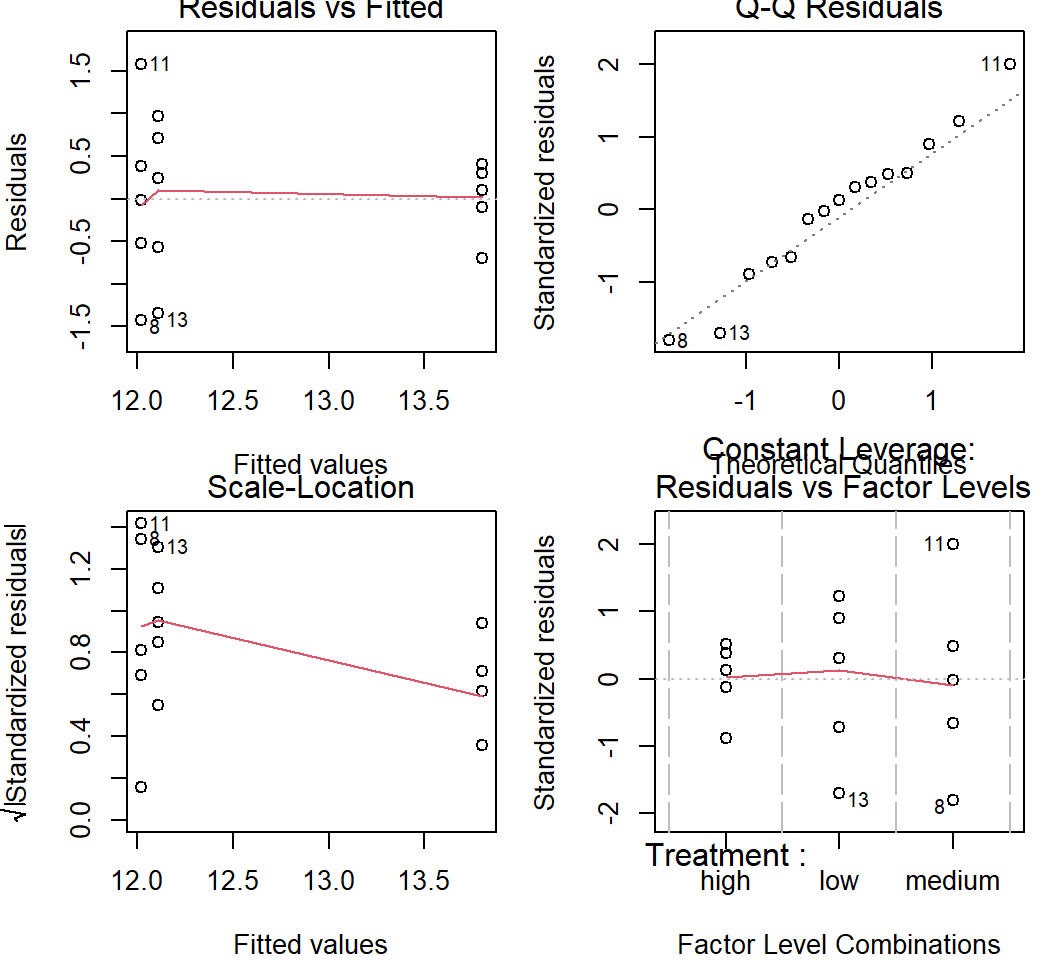
\includegraphics[width=0.5\linewidth,height=0.5\textheight]{_main_files/figure-latex/algae-aov-1} 

}

\caption{Residual plots from one-way ANOVA.}\label{fig:algae-aov}
\end{figure}

\textbf{Interpretation of residual patterns:}

\begin{itemize}
\tightlist
\item
  \textbf{Upper left:} Residuals v. fitted. This is the residual values against the fitted values. The fitted values are the means of the three groups (remember that ANOVA is about comparing means). The spread for the lower values (low and medium light) is higher than for the high light so this might make us consider the homoscedasticity assumption.\\
\item
  \textbf{Upper right:} Normal Q-Q plot. This assesses the normality assumption. The points (each point is an observation) lie around the straight line so this assumption is reasonable. Note that general linear models assume that the means of groups are normally distributed, and this always applies when the means are based on large sample sizes (roughly \(n > 30\))). When \(n < 30\), you should check that the distribution of the residuals is reasonably `normal'.\\
\item
  \textbf{Lower left:} Scale-location. This specifically looks to assess whether residuals increase with fitted values, which is a common issue in these types of analysis. In this case, the scale decreases with fitted value. This is similar to the Upper Left plot, but with \texttt{sqrt(abs(standardized\_residuals))} on the y-axis instead of just \texttt{residuals} to focus just on the magnitude of the residuals.\\
\item
  \textbf{Lower right:} Constant leverage, residuals vs.~factor levels. This indicates how each treatment is fitted (i.e.~the residuals associated with each treatment). You might be concerned if one particular treatment was associated with extremely high residuals (outliers). R automatically identifies potential outliers (8, 11, and 13 in this case) for you to further assess. In this case there is nothing in particular to worry about.
\end{itemize}

The residual plots allow you to investigate different aspects of the data and the how their assumptions are met. The interpretation of the plots overlaps in the sense that the same issue might be apparent in several of the plots.

\emph{Q166. What are the `fitted values' for an ANOVA?}

\emph{Q167. Are your effects fixed or random?}

\emph{Q168. Assuming you have chosen} \(\alpha = 0.05\)\emph{, what might you be interested in going on to test next? Hint: you are testing to see whether the means of three populations are different.}

Everything looks ok, so we can then look at the results of the ANOVA.

\begin{Shaded}
\begin{Highlighting}[]
\CommentTok{\# anova(algae\_aov) \# outputs an anova{-}type table, but unnecessary with aov()}
\FunctionTok{summary}\NormalTok{(algae\_aov)}
\end{Highlighting}
\end{Shaded}

\begin{verbatim}
##             Df Sum Sq Mean Sq F value Pr(>F)  
## Treatment    2 10.050   5.025   6.487 0.0123 *
## Residuals   12  9.296   0.775                 
## ---
## Signif. codes:  0 '***' 0.001 '**' 0.01 '*' 0.05 '.' 0.1 ' ' 1
\end{verbatim}

Reporting that there are `significant' differences between means is not enough. What your readers should be interested in is what the differences between the means actually are, and how confident you are in your assessment. This can be provided by the Tukey test in R.

\begin{Shaded}
\begin{Highlighting}[]
\NormalTok{algae\_grp\_diffs }\OtherTok{\textless{}{-}} \FunctionTok{TukeyHSD}\NormalTok{(}\AttributeTok{x =}\NormalTok{ algae\_aov, }\AttributeTok{conf.level =} \FloatTok{0.95}\NormalTok{) }
\CommentTok{\# HSD stands for \textquotesingle{}honestly significant difference\textquotesingle{}}
\NormalTok{algae\_grp\_diffs}
\end{Highlighting}
\end{Shaded}

\begin{verbatim}
##   Tukey multiple comparisons of means
##     95% family-wise confidence level
## 
## Fit: aov(formula = Yield ~ Treatment, data = algae_df)
## 
## $Treatment
##                    diff       lwr        upr     p adj
## low-high    -1.68922461 -3.174304 -0.2041449 0.0260570
## medium-high -1.78000000 -3.265080 -0.2949203 0.0194474
## medium-low  -0.09077539 -1.575855  1.3943043 0.9854641
\end{verbatim}

You can see that the mean yield at the high light level is higher than at both the low and medium: the 95\% confidence interval of the difference in comparing high and low light levels are 1.69 (0.205, 3.17) \(\mu g\) C \(ml^{-1}\). (I've inverted the results so the the difference is seen as positive (high - low rather than low - high)). This confidence interval is much more important than any P-values and you should report both (CI because it is useful, P value by convention).

\hypertarget{two-way-anova}{%
\subsection{Two-way ANOVA}\label{two-way-anova}}

You've had a look at one-way ANOVA (i.e., one predictor), which is a good starting point. However, in nature you often find numerous factors combine to influence an outcome. This is called an `interaction'. Two-way ANOVA allows you to investigate the nature of this interaction term. You can also get three-way ANOVA and more, but these get logistically challenging because you need to replicate across each level. The interpretation also gets increasingly difficult. You need to be aware of the existence of two-way ANOVA and what it offers, and how to interpret simple graphics (below), but we do not cover implementation of two-way ANOVA.

\begin{figure}
\centerline{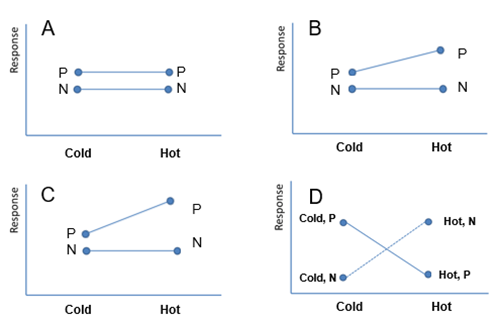
\includegraphics[width=0.6\textwidth]{figs/interactions.png}}
\caption{Graphic illustrating differing levels of interaction on the response from two treatments A and B.}
\label{fig:interaction}
\end{figure}

In Fig. \ref{fig:interaction} we have the outcome of an experiment. Each dot on the plot represents the mean Response (e.g.~growth) of a number of replicates, subject to the combination of Temperature (cold and hot) and Nutrient (N and P). We are interested in the main effects (Temp and Nutrient) and their interaction (Temp * Nutrient) In panel A, there is no effect of Temp on the Response (the lines between Cold and Hot are horizontal), but there is a main effect of Nutrient (P is higher than N). In B, there is an effect of Temp (Hot is, on average higher than Cold) but there is also an interaction as the effect of Hot is more for P than for N (where it has no effect in this example). In C, the interaction is stronger compared with B. In D, there are no treatment main effects because mean Cold = mean Hot and mean N = mean P, but there is a very strong interaction effect; the effect of Temp is reversed by Nutrient, so that the level of Nutrient (N or P) determines the effect of Temp. When it is Cold the Response is high for Nutrient P and low for Nutrient N, when it is Hot, the Response is low for Nutrient P and high for Nutrient N (but the average for hot=cold, and average for N=P)

\begin{center}\rule{0.5\linewidth}{0.5pt}\end{center}

\hypertarget{regression}{%
\section{Regression}\label{regression}}

Correlation and regression are used to examine the strength of association between two variables. In correlation, both variables are measured (and therefore associated with measurement error). In regression, one variable is fixed (by the experimenter) and is asssumed to have no `error' associated with it and the other, called the `response variable', is measured (so has measurement error). You must be able to distinguish which of correlation or regression analyses are most appropriate.

Correlation analysis is used to measure association, where you are not attempting to formally link cause-and-effect. Regression analysis is generally used where you have experimentally manipulated the fixed factor and are looking at the response in another factor. Causation is implicit in inferential regression analysis (correlation analysis is often used in `exploratory' data analysis where any link between cause-and-effect is inherently more speculative).

The media often misreport science because it is difficult to resist the impulse to attribute causation. An overwhelming number of spurious correlations (i.e., those \emph{clearly} having no causal relationship) are documented on \href{https://tylervigen.com/spurious-correlations}{tylervigen.com}.

\hypertarget{overview-1}{%
\subsection{Overview}\label{overview-1}}

Regression is at the heart of linear models. ANOVA and t-tests are, basically, special cases of linear regression models. The regression coefficient is a measure of the strength of the relationship between the dependent variable (the one you measure) and the independent variable (the one you fix like a fixed factor in ANOVA). The regression coefficient is denoted by \(R^2\) compared with \(r\) in correlation. The regression coefficient \(R^2\) ranges from 0 to 1 (unlike \(r\) which ranges from -1 to 1). A value \(R^2 = 0\) indicates no relationship to the independent variable while \(R^2=1\) indicates that the independent variable is entirely responsible for the variability in the measured variable.

As usual, null hypothesis significance testing is often applied to regression statistics. As usual, the null hypothesis being tested is usually ``there is no functional relationship between the response and the predictor'' and this is usually conceptually nonsense. In conducting regression analysis, your objective is to quantify to the most appropriate precision and accuracy possible the relationship between X (the aspect you control, the predictor, plotted on the X axis) and Y (the variable you measure, the response, plotted on the Y axis). Your objective is to quanitfy this relationship, put confidence intervals on it, and then interpret your findings in relation to the objectives of the study and in relation to other research.

\emph{Q169. Sketch a graph demonstrating the null hypothesis (of no relationship) in regression analysis.}
\newline
\newline
\newline
\newline
\newline

Let us now consider an example in which cause and effect does exist. The data in worksheet `Regression1' shows the weight loss in \emph{Tribolium confusum}, the confused flour beetle, at different relative humidities (data from Sokal and Rohlf, 1995). The relative humidity (RH) to which the beetles are exposed can be fixed and the weight loss (via evaporative losses) of the beetles then assessed. There is no way that the null hypothesis can be true in this case: humidity will obviously influence weight loss in beetles.

\emph{Q170. In this case, what is your response variable (what are you measuring) and your predictor (i.e.~what is it that you are manipulating to determine the extent of the response)?}

\emph{Q171. Plot the data in R and check your prediction. In this case, the predictor must be displayed on the x-axis and the response must be on the y-axis.}

We are interested in whether the whole data set can be usefully represented by a linear regression relationship. We wish to estimate the relationship, and put a confidence interval on our estimate. Common sense tells us that there \emph{is} some sort of relationship (testing a null hypothesis is not very useful) but it might go in either direction (positive or negative) and we don't know the strength (i.e.~slope) of that relationship.

\hypertarget{linear-regression-in-r}{%
\subsection{Linear regression in R}\label{linear-regression-in-r}}

In R we can use a variety of techniques to conduct linear regression. The easiest is to use \texttt{lm()}. It is worth noting that \texttt{lm()} would also work for all your other general linear models (e.g.~ANOVA). They are, in fact, the same model, it is just the default output (and necessary input formatting) that differs. Try reproducing the ANOVAs above with \texttt{anova(lm(...))}.

Import data and begin:

\begin{Shaded}
\begin{Highlighting}[]
\NormalTok{beetle\_df }\OtherTok{\textless{}{-}} \FunctionTok{read\_excel}\NormalTok{(}\StringTok{"data/practical\_6.xlsx"}\NormalTok{, }\AttributeTok{sheet =} \StringTok{"Beetles"}\NormalTok{)}
\CommentTok{\# inspect the dataframe, then make a scatter plot}
\FunctionTok{par}\NormalTok{(}\AttributeTok{mfrow=}\FunctionTok{c}\NormalTok{(}\DecValTok{1}\NormalTok{,}\DecValTok{1}\NormalTok{))}
\FunctionTok{plot}\NormalTok{(WeightLoss\_Mg }\SpecialCharTok{\textasciitilde{}}\NormalTok{ Humidity, }\AttributeTok{data =}\NormalTok{ beetle\_df) }
\end{Highlighting}
\end{Shaded}

\begin{center}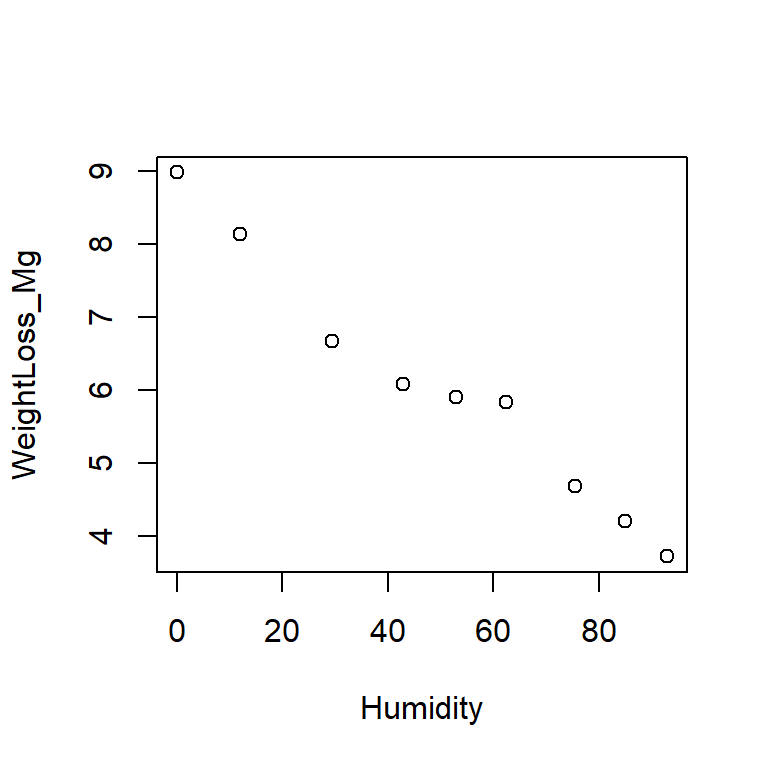
\includegraphics[width=0.4\linewidth,height=0.5\textheight]{_main_files/figure-latex/beetle-scatter-1} \end{center}

An aside on plotting: you can provide \texttt{plot()} with either a vector for the x-axis and a vector for the y-axis (i.e., \texttt{plot(x\_var,\ y\_var)}) \emph{or} you can use a formula, specifying the dataframe (i.e., \texttt{plot(y\ \textasciitilde{}\ x,\ data=data\_df)}). Just be aware of which variable is on which axis.

Now we have explored and plotted the data we can conduct the regression analysis.

\begin{Shaded}
\begin{Highlighting}[]
\CommentTok{\# weightloss is modelled as (\textasciitilde{}) a function of humidity}
\NormalTok{beetle\_lm }\OtherTok{\textless{}{-}} \FunctionTok{lm}\NormalTok{(WeightLoss\_Mg }\SpecialCharTok{\textasciitilde{}}\NormalTok{ Humidity, }\AttributeTok{data =}\NormalTok{ beetle\_df) }
\CommentTok{\# beetle\_lm}
\CommentTok{\# str(beetle\_lm) \# lm outputs are complex structures}
\end{Highlighting}
\end{Shaded}

Before we go on and interpret the model output we need to assess the model assumptions. This is done in the same way as for ANOVA with the same commands.

\begin{Shaded}
\begin{Highlighting}[]
\FunctionTok{par}\NormalTok{(}\AttributeTok{mfrow =} \FunctionTok{c}\NormalTok{(}\DecValTok{2}\NormalTok{, }\DecValTok{2}\NormalTok{), }\AttributeTok{mar=}\FunctionTok{c}\NormalTok{(}\DecValTok{4}\NormalTok{,}\DecValTok{4}\NormalTok{,}\DecValTok{1}\NormalTok{,}\DecValTok{1}\NormalTok{)) }\CommentTok{\# set up 4 in 1 plot.}
\FunctionTok{plot}\NormalTok{(beetle\_lm) }\CommentTok{\# plot the regresssion residuals.}
\end{Highlighting}
\end{Shaded}

\begin{center}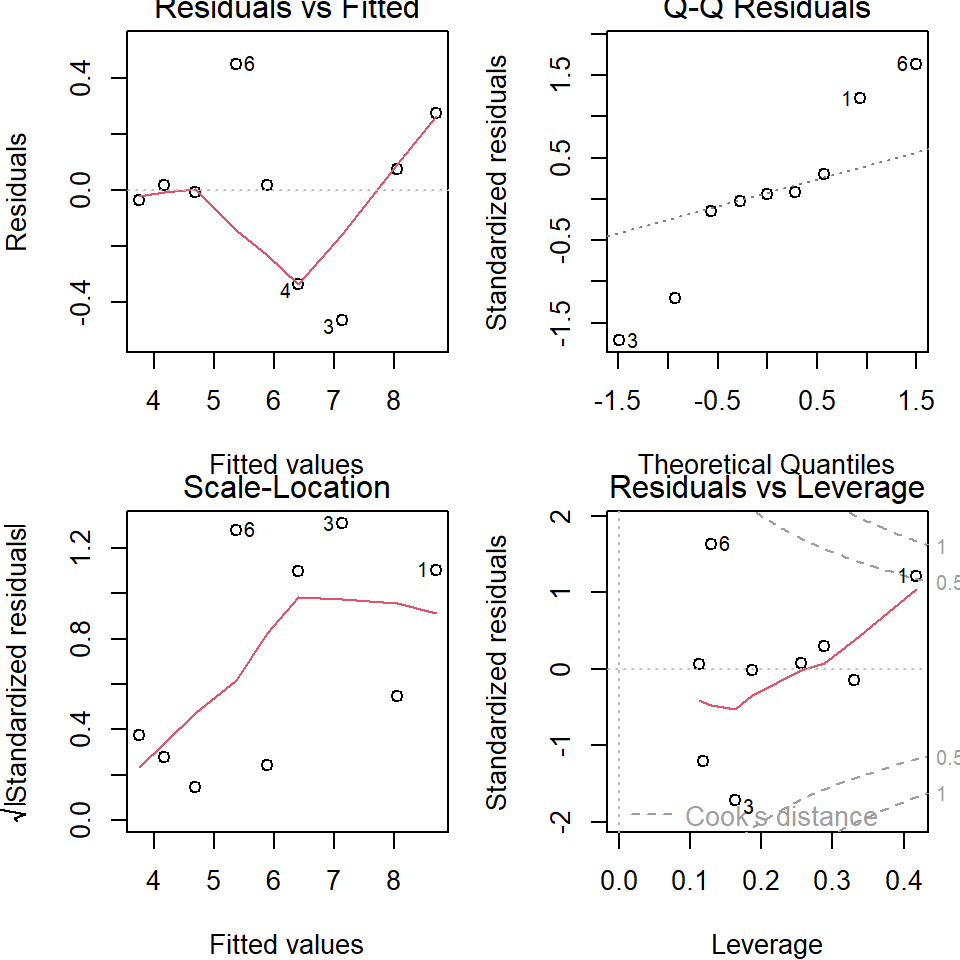
\includegraphics[width=0.5\linewidth,height=0.5\textheight]{_main_files/figure-latex/beetle-diag-1} \end{center}

The small sample size here (\(n=9\)) makes a proper analysis of the residuals difficult. The plot should be assessed in the same way as for the ANOVA residuals. Basically, any pattern is bad. The upper left (Residuals v Fitted) doesn't cause any major concern, thought upper right (Normal QQ) indicates a possible problem. Scale-Location (lower left) is difficult to interpret but no obvious pattern is present. The Residuals v. leverage (lower right) indicates a potential issue as well. A point with a large residual (i.e.~where it is very different to that expected by the model) and with a high leverage (i.e.~at the extreme ends of the predictors range) has a large Cook's distance and has a disproportionate effect on the slope and intercept. These points should be examined in more detail.

\emph{Q172. Which point has the largest Cook's distance?}

We will now proceed to looking at the linear regression analysis results on the basis that the residuals do not raise any concerns.

\begin{Shaded}
\begin{Highlighting}[]
\FunctionTok{summary}\NormalTok{(beetle\_lm)}
\end{Highlighting}
\end{Shaded}

\begin{verbatim}
## 
## Call:
## lm(formula = WeightLoss_Mg ~ Humidity, data = beetle_df)
## 
## Residuals:
##      Min       1Q   Median       3Q      Max 
## -0.46397 -0.03437  0.01675  0.07464  0.45236 
## 
## Coefficients:
##              Estimate Std. Error t value Pr(>|t|)    
## (Intercept)  8.704027   0.191565   45.44 6.54e-10 ***
## Humidity    -0.053222   0.003256  -16.35 7.82e-07 ***
## ---
## Signif. codes:  0 '***' 0.001 '**' 0.01 '*' 0.05 '.' 0.1 ' ' 1
## 
## Residual standard error: 0.2967 on 7 degrees of freedom
## Multiple R-squared:  0.9745, Adjusted R-squared:  0.9708 
## F-statistic: 267.2 on 1 and 7 DF,  p-value: 7.816e-07
\end{verbatim}

The regression equation of the form \(y = a + bx\) can be determined. The regression equation is:

\(WeightLoss = 8.70 - 0.05322 * humidity\)

Common-sense check: the coefficient is negative. As the humidity increases, the weight loss decreases (as expected and shown in the scatter plot).

\emph{Q173. What is the effect on weight loss of increasing the relative humidity by 10\%?}

\emph{Q174. What is the weight loss, predicted by the model, when relative humidity is 0\%?}

\emph{Q175. What does the model suggest the weight loss will be when relative humidity is -50\% and +150\%? Are these values sensible? What does this tell you about extrapolating beyond the data range in using regression analysis in predictions?}

The residual error is the variance in y around the line. The \(R^2\) is the proportion of this variance that is explained by the regression line. In the current case \(R^2 = 0.97\). This is an extremely high value and indicates that the regression model is extraordinarily good at accounting for the variance in weight loss based on the relative humidity.

The P values allow us to assess if the slope and the intercept are likely different from zero.

\emph{Q176. Given the very high} \(R^2\) \emph{(and looking at your plot) would you expect the regression model to be significantly better than the null model in explaining the variance in weight loss?}

\emph{Q177. With} \(\alpha = 0.05\)\emph{, do you reject or accept the null hypothesis? What would you wish to report in relation to the slope coefficient if you were reporting the results from this analysis?}

\begin{Shaded}
\begin{Highlighting}[]
\FunctionTok{confint}\NormalTok{(beetle\_lm)}
\end{Highlighting}
\end{Shaded}

\begin{verbatim}
##                   2.5 %      97.5 %
## (Intercept)  8.25104923  9.15700538
## Humidity    -0.06092143 -0.04552287
\end{verbatim}

The confidence intervals are, again, `clunky' to describe. What the above table indicates is that, if alternate yous (like in a multiverse) repeated your experiment with the same sample size, you would expect the intercept of the line to lie between 8.25 and 9.16 (3 sf) in 95\% of those replicates, and you would expect the slope to vary between -0.0455 and -0.0609. The confidence interval is the scientifically interesting bit rather than the P value.

\hypertarget{plotting-the-regression-line-and-confidence-intervals}{%
\subsection{Plotting the regression line and confidence intervals}\label{plotting-the-regression-line-and-confidence-intervals}}

A regression model (i.e.~the linear relationship between the predictor and response variables) allows us to predict values for any value of the predictor, along with confidence levels. We can plot this regression line without too much effort.

\begin{Shaded}
\begin{Highlighting}[]
\NormalTok{beetle\_pred }\OtherTok{\textless{}{-}} \FunctionTok{predict}\NormalTok{(beetle\_lm, }\AttributeTok{interval =} \StringTok{"confidence"}\NormalTok{, }\AttributeTok{level =} \FloatTok{0.95}\NormalTok{)}

\FunctionTok{par}\NormalTok{(}\AttributeTok{mfrow=}\FunctionTok{c}\NormalTok{(}\DecValTok{1}\NormalTok{,}\DecValTok{1}\NormalTok{))}
\FunctionTok{plot}\NormalTok{(WeightLoss\_Mg }\SpecialCharTok{\textasciitilde{}}\NormalTok{ Humidity, }\AttributeTok{data =}\NormalTok{ beetle\_df, }
     \AttributeTok{xlab =} \StringTok{"Relative humidity (\%)"}\NormalTok{, }\AttributeTok{ylab =} \StringTok{"Weight loss (mg)"}\NormalTok{) }
\FunctionTok{lines}\NormalTok{(beetle\_df}\SpecialCharTok{$}\NormalTok{Humidity, beetle\_pred[, }\StringTok{"fit"}\NormalTok{])}
\FunctionTok{lines}\NormalTok{(beetle\_df}\SpecialCharTok{$}\NormalTok{Humidity, beetle\_pred[, }\StringTok{"lwr"}\NormalTok{], }\AttributeTok{lty =} \DecValTok{2}\NormalTok{)}
\FunctionTok{lines}\NormalTok{(beetle\_df}\SpecialCharTok{$}\NormalTok{Humidity, beetle\_pred[, }\StringTok{"upr"}\NormalTok{], }\AttributeTok{lty =} \DecValTok{2}\NormalTok{)}
\end{Highlighting}
\end{Shaded}

\begin{figure}

{\centering 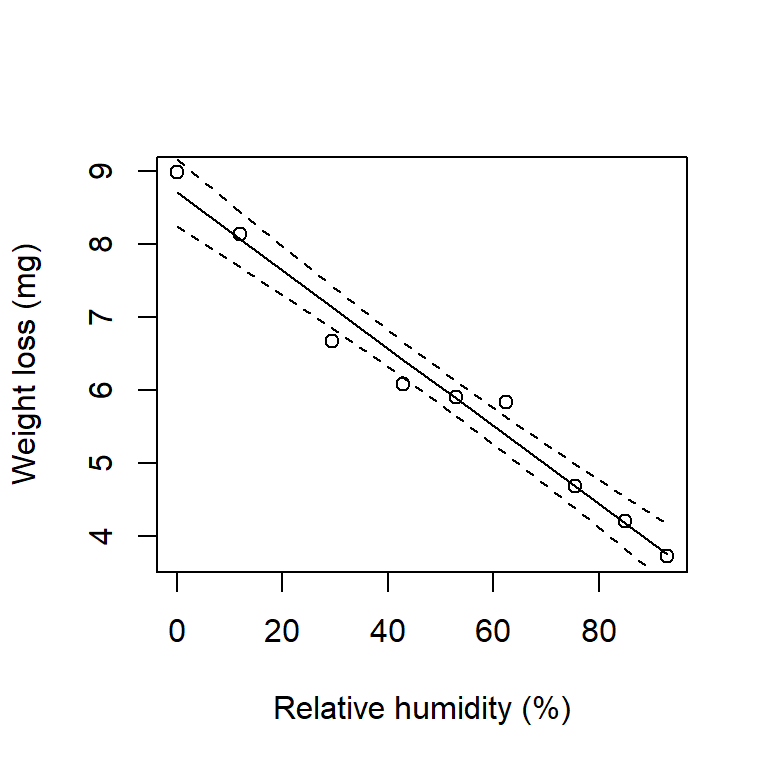
\includegraphics[width=0.5\linewidth,height=0.5\textheight]{_main_files/figure-latex/beetle-regline-1} 

}

\caption{Regression line (solid) with upper and lower 95\% CI (dashed)}\label{fig:beetle-regline}
\end{figure}

Try generating 90\% confidence intervals and add them to the plot.

\emph{Q178. Which will have the wider interval, a 99.99\% interval or a 50\% interval and why?}

\emph{Q179. Do the confidence intervals in Fig. \ref{fig:beetle-regline} run parallel to the regression line?}

\emph{Q180. If not, what does this suggest about the degree of confidence you have in values predicted at various points along the line?}

\emph{Q181. At what value of relative humidity are your predictions of weight loss likely most accurate?}

We can make predictions based on our regression line, and put confidence intervals on those predictions. Say we had a relative humidity of 50\% in the above example. You could ask for the model-predicted weight loss and you'd want confidence intervals on that prediction.

\begin{Shaded}
\begin{Highlighting}[]
\CommentTok{\# predict() needs a data.frame with the same predictors used in beetle\_lm}
\FunctionTok{predict}\NormalTok{(beetle\_lm, }
        \AttributeTok{newdata =} \FunctionTok{data.frame}\NormalTok{(}\AttributeTok{Humidity =} \DecValTok{50}\NormalTok{), }
        \AttributeTok{interval =} \StringTok{"predict"}\NormalTok{, }
        \AttributeTok{level =} \FloatTok{0.95}\NormalTok{)}
\end{Highlighting}
\end{Shaded}

\begin{verbatim}
##       fit      lwr      upr
## 1 6.04292 5.303471 6.782368
\end{verbatim}

\begin{Shaded}
\begin{Highlighting}[]
\CommentTok{\# or more fully:}
\FunctionTok{predict}\NormalTok{(beetle\_lm, }
        \AttributeTok{newdata =} \FunctionTok{data.frame}\NormalTok{(}\AttributeTok{Humidity =} \FunctionTok{seq}\NormalTok{(}\DecValTok{0}\NormalTok{, }\DecValTok{100}\NormalTok{, }\AttributeTok{by=}\DecValTok{25}\NormalTok{)), }
        \AttributeTok{interval =} \StringTok{"predict"}\NormalTok{, }
        \AttributeTok{level =} \FloatTok{0.95}\NormalTok{)}
\end{Highlighting}
\end{Shaded}

\begin{verbatim}
##        fit      lwr      upr
## 1 8.704027 7.868990 9.539064
## 2 7.373474 6.608630 8.138317
## 3 6.042920 5.303471 6.782368
## 4 4.712366 3.949031 5.475701
## 5 3.381812 2.549540 4.214084
\end{verbatim}

These are prediction intervals and they are broader than confidence intervals. The confidence intervals express your confidence about where the mean regression line would lie (if you went back in time and were somehow able to repeatedly sample from the same population). The prediction interval expresses your confidence about where the \emph{values} would lie if you went back and repeatedly took an individual of the population at a given value of the predictor (e.g.~50\% humidity).
For more kicks, import PhosphateCalibration (1st year practical data) into R and duplicate the following plots and confidence intervals.

\begin{Shaded}
\begin{Highlighting}[]
\NormalTok{phosphate\_df }\OtherTok{\textless{}{-}} \FunctionTok{read\_xlsx}\NormalTok{(}\StringTok{"data/Practical\_6.xlsx"}\NormalTok{, }\StringTok{"PhosphateCalibration"}\NormalTok{)}
\end{Highlighting}
\end{Shaded}

\begin{center}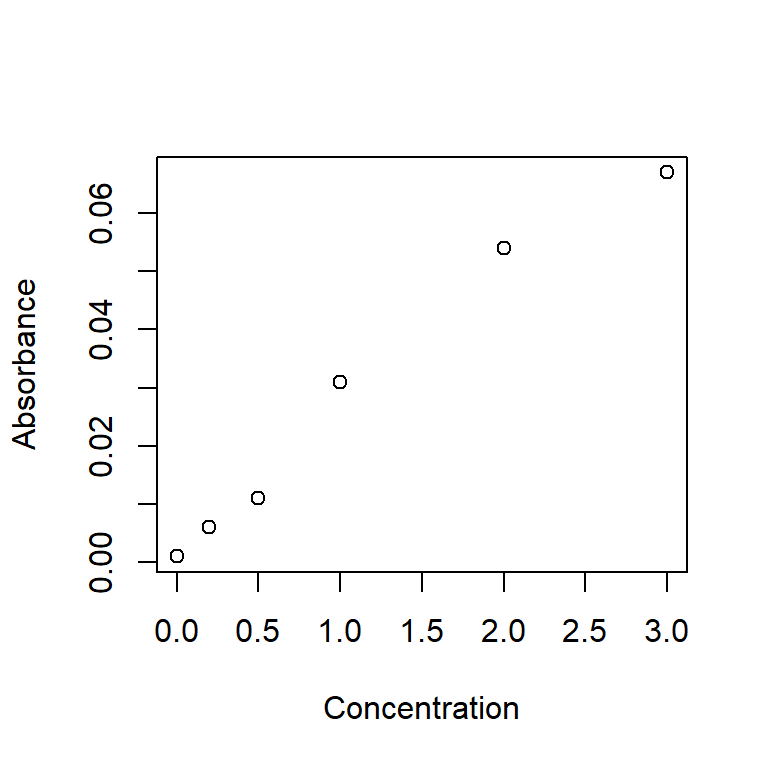
\includegraphics[width=0.5\linewidth,height=0.5\textheight]{_main_files/figure-latex/unnamed-chunk-80-1} \end{center}

\begin{center}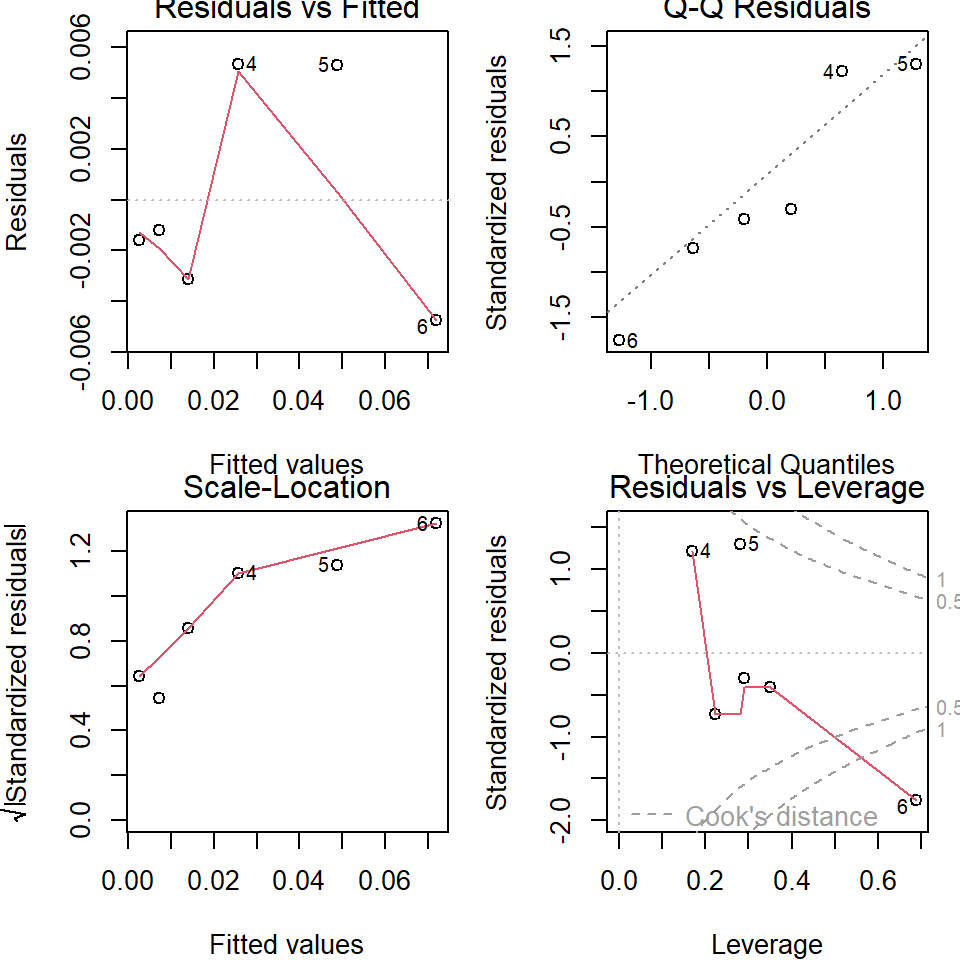
\includegraphics[width=0.5\linewidth,height=0.5\textheight]{_main_files/figure-latex/unnamed-chunk-81-1} \end{center}

\begin{verbatim}
## 
## Call:
## lm(formula = Absorbance ~ Concentration, data = phosphate_df)
## 
## Residuals:
##         1         2         3         4         5         6 
## -0.001605 -0.001213 -0.003125  0.005355  0.005314 -0.004726 
## 
## Coefficients:
##               Estimate Std. Error t value Pr(>|t|)    
## (Intercept)   0.002605   0.002853   0.913 0.412856    
## Concentration 0.023040   0.001849  12.464 0.000238 ***
## ---
## Signif. codes:  0 '***' 0.001 '**' 0.01 '*' 0.05 '.' 0.1 ' ' 1
## 
## Residual standard error: 0.004823 on 4 degrees of freedom
## Multiple R-squared:  0.9749, Adjusted R-squared:  0.9686 
## F-statistic: 155.3 on 1 and 4 DF,  p-value: 0.0002383
\end{verbatim}

\emph{Q182. Are you happy with your model assumptions?}

\emph{Q183. Write down the regression equation.}

\emph{Q184. Determine the confidence interval for the regression line.}

\emph{Q185. For a concentration of 0.75 units, what values would you expect (95 times in 100) to see from your experimental set-up?}

You should get:

\begin{verbatim}
##          fit         lwr        upr
## 1 0.01988519 0.005298129 0.03447225
\end{verbatim}

\begin{center}\rule{0.5\linewidth}{0.5pt}\end{center}

\hypertarget{conclusions-4}{%
\section{Conclusions}\label{conclusions-4}}

Correlation is a measure of association between two variables. It is appropriate to use correlation to measure this association when one cannot or does not wish to assume that any relationship is causative. Pearson correlation coefficients should only be used where it is fair to assume (by looking at scatter plot) that the relationship is approximatley linear. Where linearity does not apply, attempt to transform one or both of the variables. Where there are outliers (that cannot be removed) or where one is uncertain about some of the data, then non-parametric ranked based correlation coefficients, such as the Spearman coefficient, should be used. As with GLMs, correlation analysis assumes that all points are independent of each other.

Linear regression is one of the most widely used statistical techniques. It is used to examine causal relationships, often where experimental manipulations are conducted. Regression is a general linear model and it lies within the generalised linear model family (GLMs). GLMs allow you to model data that is not normally distributed, including proportions (bounded by 0 and 1), or counts (bounded by 0). Using a GLM is a much better way of analysing these data compared with transforming the response variable or using non-parametric techniques. All members of the GLM family make the assumptions that measurements are independent of each other. Where this assumption fails you can use generalised linear mixed models (GLMMs). Extensions of simple linear regression include multiple regression which examines the influence of two or more continuous variables on a response variable.

\hypertarget{multivariate}{%
\chapter{Multivariate analysis}\label{multivariate}}

So far, every model we've used has had a single response variable. Multivariate analyses expand this to allow the analysis of, for example, counts of each species within a community. Statistical routines for multivariate analysis are relatively new and have co-evolved with computational capacity over the last 50 years or so. Multivariate data typically take the form of a matrix of samples (each row is a sample) v `features' (columns). Features may include things like faunal counts, chemical concentrations, or environmental conditions.

Multivariate analysis typically includes three stages: 1) data transformation or standardisation, 2) generation of a dissimilarity matrix and, 3) ordination (display) of that matrix. Each of these elements has numerous options, with advantages and disadvantages to each. Multivariate analysis are less inferential than most univariate approaches and implementation can feel like a `black-art'! Statisticians are still arguing about the best way to approach multivariate analyses.

Multivariate data, such as species inventories, have been recorded for centuries and form a critical resource. Multivariate time series data are particularly important for assessing relative change that might be attributable to man's activities, for example in relation to climate or land-use change. The `internet of things', the generation of multiple data-streams from the same station (e.g.~a glider with CTD), and the development of bioinformatics (e.g.~metabarcoding) all lend themselves to multivariate analyses.

More detail on the the material we cover here is given in \href{https://www.primer-e.com/wp-content/uploads/2018/10/Change-in-Marine-Communities-3rd-ed.pdf}{Clarke et al.~2014. Change in marine communities: An approach to statistical analysis and interpretation.}. If that link does not work, you can try navigating to the \href{https://www.primer-e.com/download/}{PRIMER-e downloads page}, fill out your info to download the Manuals, then select ``Change in Marine Communities''. Unfortunately, the PRIMER software developed by the authors is not free. Instead, we'll use our gloriously free and open source R.

\hypertarget{multivariate-analysis-in-r}{%
\section{Multivariate analysis in R}\label{multivariate-analysis-in-r}}

For the non-metric NMDS workflow, we'll start by simulating some data. Then, we'll transform the data (`log' and fourth-root) and generate dissimilarity matrices from this transformed data. Finally, we'll plot it using NMDS. We'll generate diversity indices with our simulated data, then have a look at some real data (available via the package \emph{vegan}).

For the PCA workflow, we'll have a look at some environmental data using PCA. Throughout this practical, we'll illustrate some coding techniques which will help you practice wrangling your data to make it suitable for analysis. As we've discussed, data wrangling is a time-consuming and crucial part of data analysis so familiarity with this is essential.

Recall from Section @ref\{normal\} that the \texttt{\^{}} operator raises each element in a vector to a power. For example, say we create a vector \texttt{obs\_values\ \textless{}-\ c(1,\ 10,\ 35)}. We can calculate a fourth-root transformation of the whole vector with \texttt{obs\_values\^{}(1/4)}. Remember from previous courses that this is identical to \texttt{sqrt(sqrt(obs\_values))}.

\begin{Shaded}
\begin{Highlighting}[]
\FunctionTok{library}\NormalTok{(vegan) }
\CommentTok{\# these toy data duplicate those in the multivariate lecture.}
\NormalTok{worm\_df }\OtherTok{\textless{}{-}} \FunctionTok{data.frame}\NormalTok{(}
  \AttributeTok{row.names =} \FunctionTok{c}\NormalTok{(}\StringTok{"CE1"}\NormalTok{, }\StringTok{"CE2"}\NormalTok{, }\StringTok{"Ref1"}\NormalTok{, }\StringTok{"Ref2"}\NormalTok{),}
  \AttributeTok{Capitella =} \FunctionTok{c}\NormalTok{(}\DecValTok{1000}\NormalTok{, }\DecValTok{1500}\NormalTok{, }\DecValTok{10}\NormalTok{, }\DecValTok{50}\NormalTok{),}
  \AttributeTok{Malacoeros =} \FunctionTok{c}\NormalTok{(}\DecValTok{500}\NormalTok{, }\DecValTok{2000}\NormalTok{, }\DecValTok{50}\NormalTok{, }\DecValTok{25}\NormalTok{),}
  \AttributeTok{Mysella =} \FunctionTok{c}\NormalTok{(}\DecValTok{1}\NormalTok{, }\DecValTok{0}\NormalTok{, }\DecValTok{25}\NormalTok{, }\DecValTok{30}\NormalTok{),}
  \AttributeTok{Nucella =} \FunctionTok{c}\NormalTok{(}\DecValTok{1}\NormalTok{, }\DecValTok{0}\NormalTok{, }\DecValTok{20}\NormalTok{, }\DecValTok{15}\NormalTok{)}
\NormalTok{)}
\NormalTok{worm\_df}
\end{Highlighting}
\end{Shaded}

\begin{verbatim}
##      Capitella Malacoeros Mysella Nucella
## CE1       1000        500       1       1
## CE2       1500       2000       0       0
## Ref1        10         50      25      20
## Ref2        50         25      30      15
\end{verbatim}

\begin{Shaded}
\begin{Highlighting}[]
\CommentTok{\# alt{-}log transformation: ifelse(x==0, 0, log(x))}
\NormalTok{worm\_df\_log }\OtherTok{\textless{}{-}} \FunctionTok{decostand}\NormalTok{(worm\_df, }\AttributeTok{method =} \StringTok{"log"}\NormalTok{, }\AttributeTok{logbase =} \DecValTok{10}\NormalTok{)}
\NormalTok{worm\_df\_4rt }\OtherTok{\textless{}{-}}\NormalTok{ worm\_df}\SpecialCharTok{\^{}}\FloatTok{0.25}
\end{Highlighting}
\end{Shaded}

Take a look at \texttt{worm\_df}, \texttt{worm\_df\_log}, and \texttt{worm\_df\_4rt} to be sure they make sense.

Next we use \texttt{vegdist()} to generate different distance matrices for the raw and transformed data. See \texttt{?vegdist} for more information. We'll use Bray-Curtis for the raw and 4\textsuperscript{th}-root transformed data, and alternative Gower for the alt-log transformed data. See the multivariate lecture area on Brightspace for details on these algorithms. Feel free to investigate other combinations of data transformation and dissimilarity matrices.

\begin{Shaded}
\begin{Highlighting}[]
\FunctionTok{vegdist}\NormalTok{(worm\_df, }\AttributeTok{method =} \StringTok{"bray"}\NormalTok{)}
\end{Highlighting}
\end{Shaded}

\begin{verbatim}
##            CE1       CE2      Ref1
## CE2  0.4002399                    
## Ref1 0.9228376 0.9667129          
## Ref2 0.9050555 0.9585635 0.3333333
\end{verbatim}

\begin{Shaded}
\begin{Highlighting}[]
\FunctionTok{vegdist}\NormalTok{(worm\_df\_4rt, }\AttributeTok{method =} \StringTok{"bray"}\NormalTok{)}
\end{Highlighting}
\end{Shaded}

\begin{verbatim}
##             CE1        CE2       Ref1
## CE2  0.18044721                      
## Ref1 0.39098221 0.59100112           
## Ref2 0.36024122 0.55728021 0.08642723
\end{verbatim}

\begin{Shaded}
\begin{Highlighting}[]
\FunctionTok{vegdist}\NormalTok{(worm\_df\_log, }\AttributeTok{method =} \StringTok{"altGower"}\NormalTok{)}
\end{Highlighting}
\end{Shaded}

\begin{verbatim}
##            CE1       CE2      Ref1
## CE2  0.6945378                    
## Ref1 1.4247425 2.1192803          
## Ref2 1.3138181 2.0083559 0.3010300
\end{verbatim}

\emph{Q140. How many combinations of transformation and dissimilarity matrix do we have already?}

\emph{Q141. Examine one or more of the dissimilarity matrices. Which sites are closer (smaller numbers) and which are futher apart (bigger numbers)? Does this align with an `eyeballing' of the data? How has the data transformation changed the resultant dissimilarity matrix?}

Next we want to plot our dissimilarities, so we can easily visualise which sites are more similar/dissimilar to each other. We will use functions from \emph{vegan} to plot the ordinations. Remember that you can run \texttt{?packageName} to learn more about any R package, typically with helpful examples and vignettes of the most useful applications of the package.

We have numerous options in relation to displaying the dissimiliarty matrices. We'll explore non-metric multiple dimensional scaling, abbreviated to NMDS, nMDS, nmMDS, or just MDS.

\emph{Q142. Use \texttt{?vegdist} to see what alternative distance measures are available.}

The \texttt{metaMDS()} function calculates a dissimilarity matrix (as we did above) and produces an R object with all the information needed for plotting. It expects that samples are in rows and species (or features) are in columns. We can also specify the distance metric, the number of axes, whether to autotransform the data, and many other options. See \texttt{?metaMDS} for the default values and other available arguments.

\begin{Shaded}
\begin{Highlighting}[]
\NormalTok{ord\_raw }\OtherTok{\textless{}{-}} \FunctionTok{metaMDS}\NormalTok{(worm\_df, }\AttributeTok{distance =} \StringTok{"bray"}\NormalTok{, }\AttributeTok{k =} \DecValTok{2}\NormalTok{,}
                   \AttributeTok{autotransform =} \ConstantTok{FALSE}\NormalTok{, }\AttributeTok{trace =} \ConstantTok{FALSE}\NormalTok{)}
\FunctionTok{ordiplot}\NormalTok{(ord\_raw, }\AttributeTok{choices =} \FunctionTok{c}\NormalTok{(}\DecValTok{1}\NormalTok{, }\DecValTok{2}\NormalTok{), }\AttributeTok{display =} \StringTok{"sites"}\NormalTok{, }
         \AttributeTok{type =} \StringTok{"text"}\NormalTok{, }\AttributeTok{main =} \StringTok{"NMDS: raw data, Bray{-}Curtis"}\NormalTok{)}
\end{Highlighting}
\end{Shaded}

\begin{figure}

{\centering 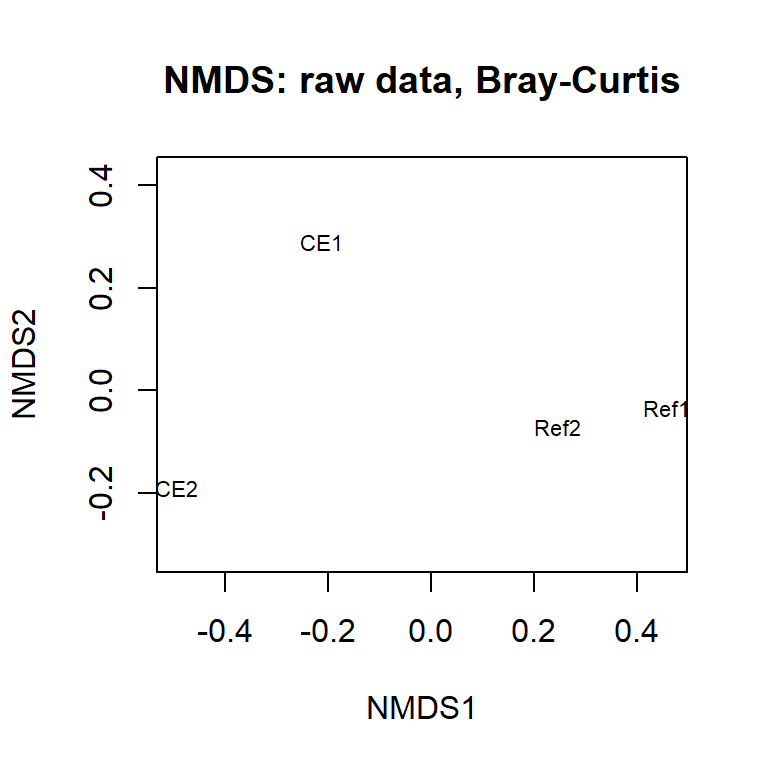
\includegraphics[width=0.4\linewidth,height=0.4\textheight]{_main_files/figure-latex/worm-1-1} 

}

\caption{Simple pattern in example worm data.}\label{fig:worm-1}
\end{figure}

Compare this with the 4\textsuperscript{th}-root transformed data using the same distance metric.

\begin{Shaded}
\begin{Highlighting}[]
\NormalTok{ord\_4rt }\OtherTok{\textless{}{-}} \FunctionTok{metaMDS}\NormalTok{(worm\_df\_4rt, }\AttributeTok{distance =} \StringTok{"bray"}\NormalTok{, }\AttributeTok{k =} \DecValTok{2}\NormalTok{, }
                   \AttributeTok{autotransform =} \ConstantTok{FALSE}\NormalTok{, }\AttributeTok{trace =} \ConstantTok{FALSE}\NormalTok{)}
\end{Highlighting}
\end{Shaded}

\emph{Q143. Plot \texttt{ord\_4rt}. How has the 4th root changed your data intepretation?}

\emph{Q144. Examine your ordination(s) and interpret, cross referencing to the raw and transformed data. Are the patterns that you see in the data apparent on the ordination?}

You can include on your plot the species `locations' (as determined by their correlation with the axes). This shows where the main associations are occurring.

\begin{Shaded}
\begin{Highlighting}[]
\CommentTok{\# you can also plot the \textquotesingle{}species\textquotesingle{} on the ordination,}
\FunctionTok{ordiplot}\NormalTok{(ord\_4rt, }\AttributeTok{choices =} \FunctionTok{c}\NormalTok{(}\DecValTok{1}\NormalTok{, }\DecValTok{2}\NormalTok{), }\AttributeTok{display =} \FunctionTok{c}\NormalTok{(}\StringTok{"sites"}\NormalTok{, }\StringTok{"species"}\NormalTok{), }
         \AttributeTok{type =} \StringTok{"text"}\NormalTok{, }\AttributeTok{main =} \StringTok{"NMDS, 4th{-}rt trans., Bray{-}Curtis"}\NormalTok{)}
\end{Highlighting}
\end{Shaded}

\begin{figure}

{\centering 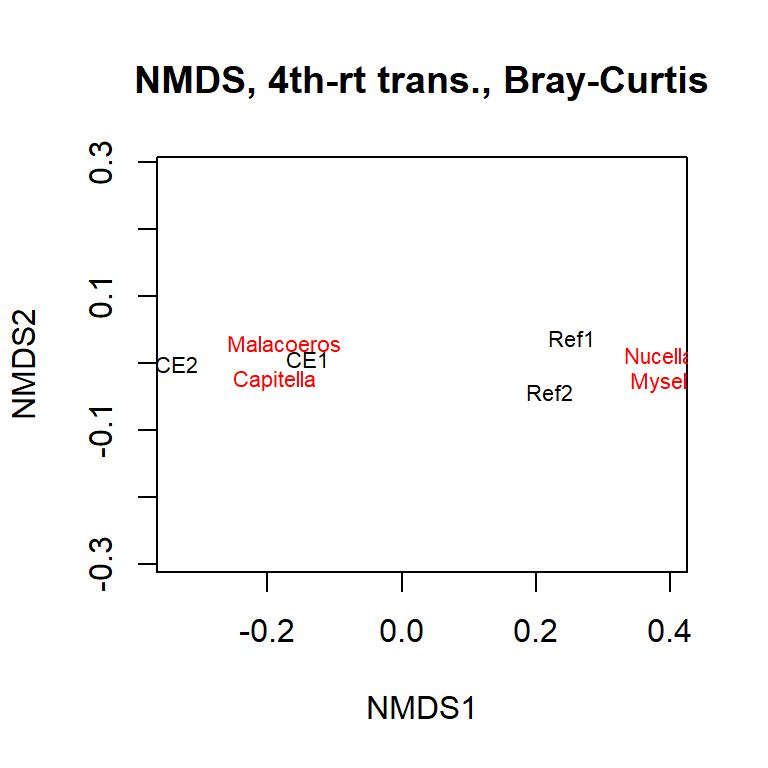
\includegraphics[width=0.4\linewidth,height=0.4\textheight]{_main_files/figure-latex/worm-2-1} 

}

\caption{Species superimposed onto ordination, indicating species-site associations.}\label{fig:worm-2}
\end{figure}

\emph{Q145. Replot the untransformed data, but this time include the species. How has the transformation changed your interpretation of the data?}

Let's have a look at another simulated dataset.

\begin{Shaded}
\begin{Highlighting}[]
\NormalTok{comm\_df }\OtherTok{\textless{}{-}} \FunctionTok{data.frame}\NormalTok{(}
  \AttributeTok{row.names =} \FunctionTok{c}\NormalTok{(}\StringTok{"Dunst"}\NormalTok{, }\StringTok{"Creran"}\NormalTok{, }\StringTok{"Lismore"}\NormalTok{, }\StringTok{"Charl"}\NormalTok{),}
  \AttributeTok{SpA =} \FunctionTok{c}\NormalTok{(}\DecValTok{1}\NormalTok{, }\DecValTok{20}\NormalTok{, }\DecValTok{30}\NormalTok{, }\DecValTok{40}\NormalTok{),}
  \AttributeTok{SpB =} \FunctionTok{c}\NormalTok{(}\DecValTok{11}\NormalTok{, }\DecValTok{22}\NormalTok{, }\DecValTok{50}\NormalTok{, }\DecValTok{1}\NormalTok{),}
  \AttributeTok{SpC =} \FunctionTok{c}\NormalTok{(}\DecValTok{500}\NormalTok{, }\DecValTok{40}\NormalTok{, }\DecValTok{30}\NormalTok{, }\DecValTok{20}\NormalTok{),}
  \AttributeTok{SpD =} \FunctionTok{c}\NormalTok{(}\DecValTok{10}\NormalTok{, }\DecValTok{25}\NormalTok{, }\DecValTok{35}\NormalTok{, }\DecValTok{50}\NormalTok{),}
  \AttributeTok{SpE =} \FunctionTok{c}\NormalTok{(}\DecValTok{4}\NormalTok{, }\DecValTok{3}\NormalTok{, }\DecValTok{2}\NormalTok{, }\DecValTok{1}\NormalTok{),}
  \AttributeTok{SpF =} \FunctionTok{c}\NormalTok{(}\DecValTok{40}\NormalTok{, }\DecValTok{250}\NormalTok{, }\DecValTok{1}\NormalTok{, }\DecValTok{9}\NormalTok{)}
\NormalTok{)}
\NormalTok{comm\_df}
\end{Highlighting}
\end{Shaded}

\begin{verbatim}
##         SpA SpB SpC SpD SpE SpF
## Dunst     1  11 500  10   4  40
## Creran   20  22  40  25   3 250
## Lismore  30  50  30  35   2   1
## Charl    40   1  20  50   1   9
\end{verbatim}

\begin{Shaded}
\begin{Highlighting}[]
\NormalTok{ord\_comm }\OtherTok{\textless{}{-}} \FunctionTok{metaMDS}\NormalTok{(comm\_df, }\AttributeTok{distance =} \StringTok{"bray"}\NormalTok{, }\AttributeTok{k =} \DecValTok{2}\NormalTok{, }
                    \AttributeTok{autotransform =} \ConstantTok{FALSE}\NormalTok{, }\AttributeTok{trace =} \ConstantTok{FALSE}\NormalTok{)}
\FunctionTok{ordiplot}\NormalTok{(ord\_comm, }\AttributeTok{choices =} \FunctionTok{c}\NormalTok{(}\DecValTok{1}\NormalTok{, }\DecValTok{2}\NormalTok{), }
         \AttributeTok{display =} \FunctionTok{c}\NormalTok{(}\StringTok{"sites"}\NormalTok{, }\StringTok{"species"}\NormalTok{), }\AttributeTok{type =} \StringTok{"text"}\NormalTok{)}
\end{Highlighting}
\end{Shaded}

\begin{figure}

{\centering 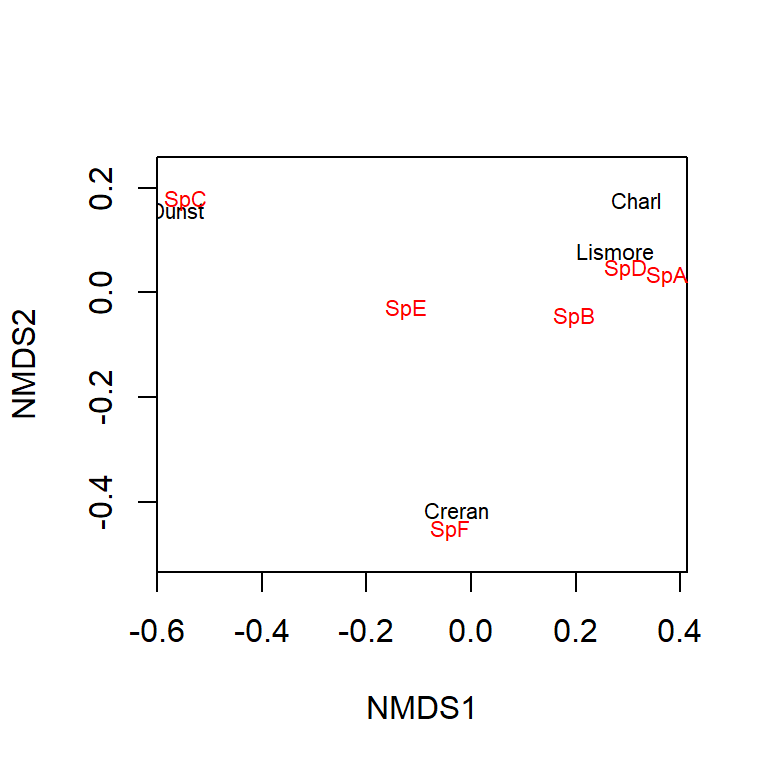
\includegraphics[width=0.4\linewidth,height=0.4\textheight]{_main_files/figure-latex/comm-ord-1} 

}

\caption{Ordination for a simulated dataset showing sites and species.}\label{fig:comm-ord}
\end{figure}

\emph{Q146. Have a look at these raw data. What are the main trends? Which sites are more similar?}

These data are still much simpler than most `real' data sets but it is still difficult to summarise the similarities and differences between stations. However, multivariate analyses help you in this process.

\emph{Q147. Now forth-root transform these data, generate the new dissimilarity matrix and plot it.}

\emph{Q148. What has the transformation done to your interpretation of differences between the Sites and Site x Species associations?}

\emph{Q149. Add a title to your graph.}

\begin{center}\rule{0.5\linewidth}{0.5pt}\end{center}

\hypertarget{diversity-indices}{%
\section{Diversity indices}\label{diversity-indices}}

Prior to the development of the multivariate techniques you'll be using today, univariate indices were derived from multivariate data. A classic example of such a univariate measure in ecology is the Shannon-Wiener diversity index (a.k.a., Shannon's H). This index balances the \emph{number} of species in a sample and the \emph{relative abundance} of each species (where `species' can once again be any sort of feature). Univariate measures of `evenness' can also be derived from multivariate data and, when reporting species data, you may also wish to include species richness, which is just the number of species present regardless of their abundances.

We can use the \texttt{comm\_df} dataset we invented to explore some diversity concepts.

\emph{Q150. Looking at the \texttt{comm\_df} data (by eye) and given the description above, which of the sites is assocaited with the lowest and highest diversity?}

\begin{Shaded}
\begin{Highlighting}[]
\NormalTok{shannon\_H }\OtherTok{\textless{}{-}} \FunctionTok{diversity}\NormalTok{(comm\_df, }\StringTok{"shannon"}\NormalTok{, }\AttributeTok{base =} \FunctionTok{exp}\NormalTok{(}\DecValTok{1}\NormalTok{)) }
\NormalTok{richness }\OtherTok{\textless{}{-}} \FunctionTok{specnumber}\NormalTok{(comm\_df) }
\FunctionTok{barplot}\NormalTok{(shannon\_H, }\AttributeTok{names.arg =}\NormalTok{ comm\_df}\SpecialCharTok{$}\NormalTok{Site, }\AttributeTok{main =} \ConstantTok{NULL}\NormalTok{, }\AttributeTok{ylab =} \StringTok{"Shannon\textquotesingle{}s H"}\NormalTok{)}
\end{Highlighting}
\end{Shaded}

\begin{figure}

{\centering 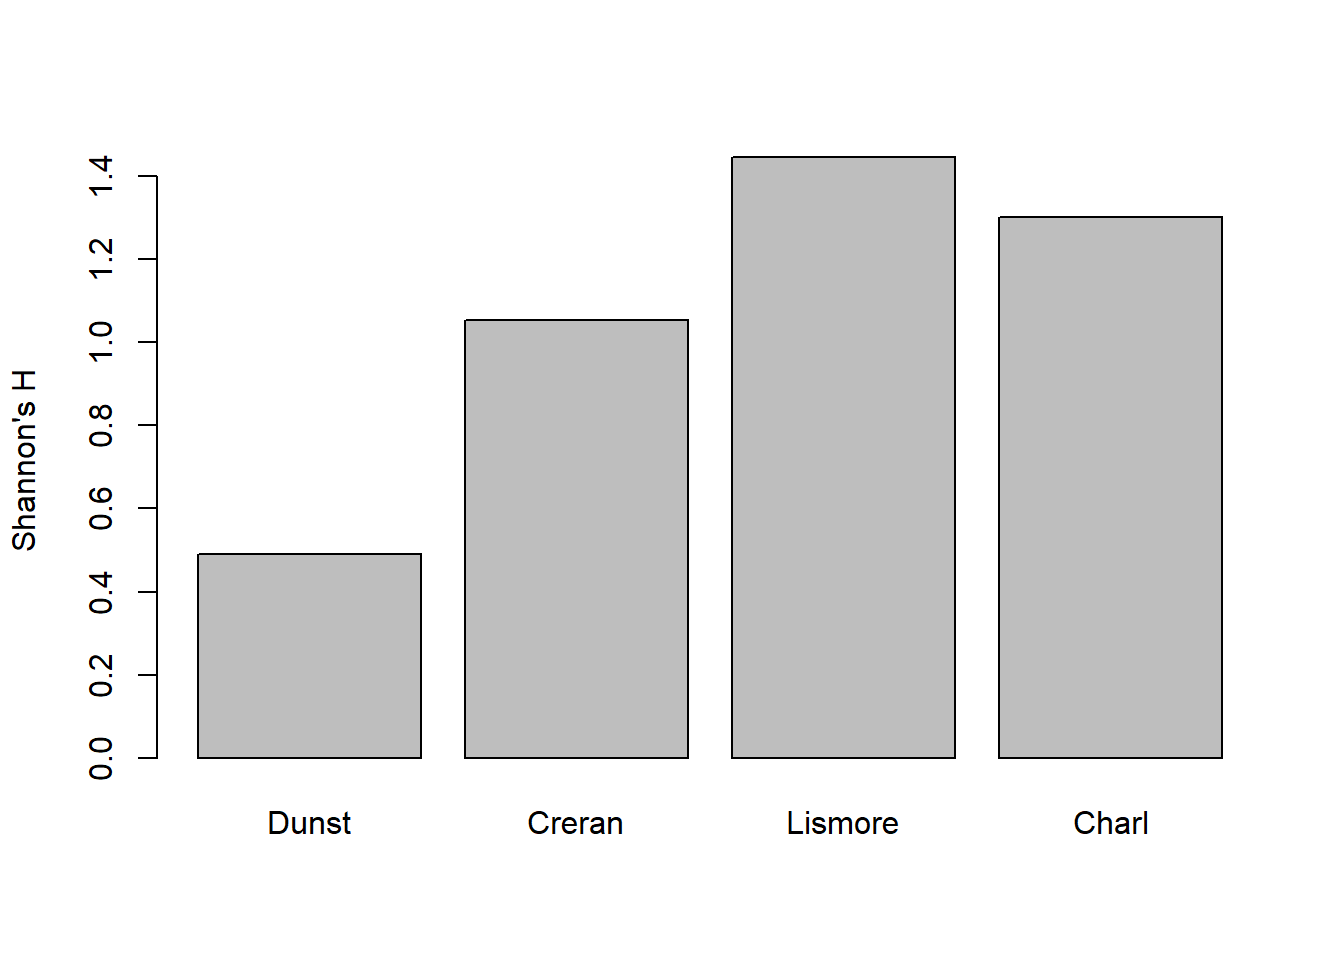
\includegraphics[width=0.5\linewidth,height=0.5\textheight]{_main_files/figure-latex/H-examp-1} 

}

\caption{Shannon diversity}\label{fig:H-examp}
\end{figure}

Try plotting \texttt{richness}.

\emph{Q151. Do the plots correspond to what you expected?}

\emph{Q152. What does \texttt{specnumber} do?}

\emph{Q153. Change \texttt{comm\_df} to introduce some very evenly distributed species across sites and some with extremes or absenses and see how this effects diversity and richness.}

\emph{Q154. How could you `counter' any extremes (as in superabundant taxa) in the raw count data that you've generated? Try your idea.}

\emph{Q155. Which description (diversity or richness) is `best' for describing your multivariate data? How does this compare to NMDS?}

\hypertarget{nmds-on-real-data}{%
\section{NMDS on real data}\label{nmds-on-real-data}}

Now you've been introduced to NMDS and diversity indices, with `fake' data, you are in a better position to interpret real data. Using simulated (or at least simple) data to learn new statistical techniques is usually the best approach because it gives you the opportunity to get a better sense for how the algorithms work (and to be sure your code is free from bugs!).

Have a look at the \texttt{varespec} and \texttt{varechem} datasets included in the \emph{vegan} package. I've reproduced the examples below:

\begin{Shaded}
\begin{Highlighting}[]
\FunctionTok{data}\NormalTok{(varespec) }\CommentTok{\# ?varespec {-}{-} percent cover of 44 spp in lichen pastures }
\FunctionTok{data}\NormalTok{(varechem) }\CommentTok{\# ?varechem {-}{-} associated soil charecteristics}
\NormalTok{ord\_vare }\OtherTok{\textless{}{-}} \FunctionTok{metaMDS}\NormalTok{(varespec}\SpecialCharTok{\^{}}\FloatTok{0.25}\NormalTok{, }\AttributeTok{distance =} \StringTok{"bray"}\NormalTok{, }
                   \AttributeTok{trace =} \ConstantTok{FALSE}\NormalTok{, }\AttributeTok{autotransform =} \ConstantTok{FALSE}\NormalTok{)}
\end{Highlighting}
\end{Shaded}

\begin{Shaded}
\begin{Highlighting}[]
\FunctionTok{par}\NormalTok{(}\AttributeTok{mfrow=}\FunctionTok{c}\NormalTok{(}\DecValTok{1}\NormalTok{,}\DecValTok{3}\NormalTok{), }\AttributeTok{mar=}\FunctionTok{c}\NormalTok{(}\DecValTok{4}\NormalTok{,}\DecValTok{4}\NormalTok{,}\DecValTok{1}\NormalTok{,}\DecValTok{1}\NormalTok{)) }
\FunctionTok{ordiplot}\NormalTok{(ord\_vare, }\AttributeTok{choices =} \FunctionTok{c}\NormalTok{(}\DecValTok{1}\NormalTok{, }\DecValTok{2}\NormalTok{), }\AttributeTok{display =} \StringTok{"sites"}\NormalTok{, }\AttributeTok{type =} \StringTok{"text"}\NormalTok{)}
\FunctionTok{ordiplot}\NormalTok{(ord\_vare, }\AttributeTok{choices =} \FunctionTok{c}\NormalTok{(}\DecValTok{1}\NormalTok{, }\DecValTok{2}\NormalTok{), }\AttributeTok{display =} \StringTok{"species"}\NormalTok{, }\AttributeTok{type =} \StringTok{"text"}\NormalTok{)}
\FunctionTok{ordiplot}\NormalTok{(ord\_vare, }\AttributeTok{choices =} \FunctionTok{c}\NormalTok{(}\DecValTok{1}\NormalTok{, }\DecValTok{2}\NormalTok{), }\AttributeTok{display =} \FunctionTok{c}\NormalTok{(}\StringTok{"sites"}\NormalTok{, }\StringTok{"species"}\NormalTok{),}
  \AttributeTok{type =} \StringTok{"text"}\NormalTok{)}
\CommentTok{\# You can superimpose environmental variables onto NMDS{-}ordinations.}
\NormalTok{ef }\OtherTok{\textless{}{-}} \FunctionTok{envfit}\NormalTok{(ord\_vare, varechem) }\CommentTok{\#}
\FunctionTok{plot}\NormalTok{(ef, }\AttributeTok{p.max =} \FloatTok{0.1}\NormalTok{, }\AttributeTok{col =} \StringTok{"green"}\NormalTok{) }\CommentTok{\# overlay environmental variables}
\FunctionTok{plot}\NormalTok{(ef, }\AttributeTok{p.max =} \FloatTok{0.01}\NormalTok{, }\AttributeTok{col =} \StringTok{"blue"}\NormalTok{) }\CommentTok{\# subset based on p}
\end{Highlighting}
\end{Shaded}

\begin{figure}

{\centering 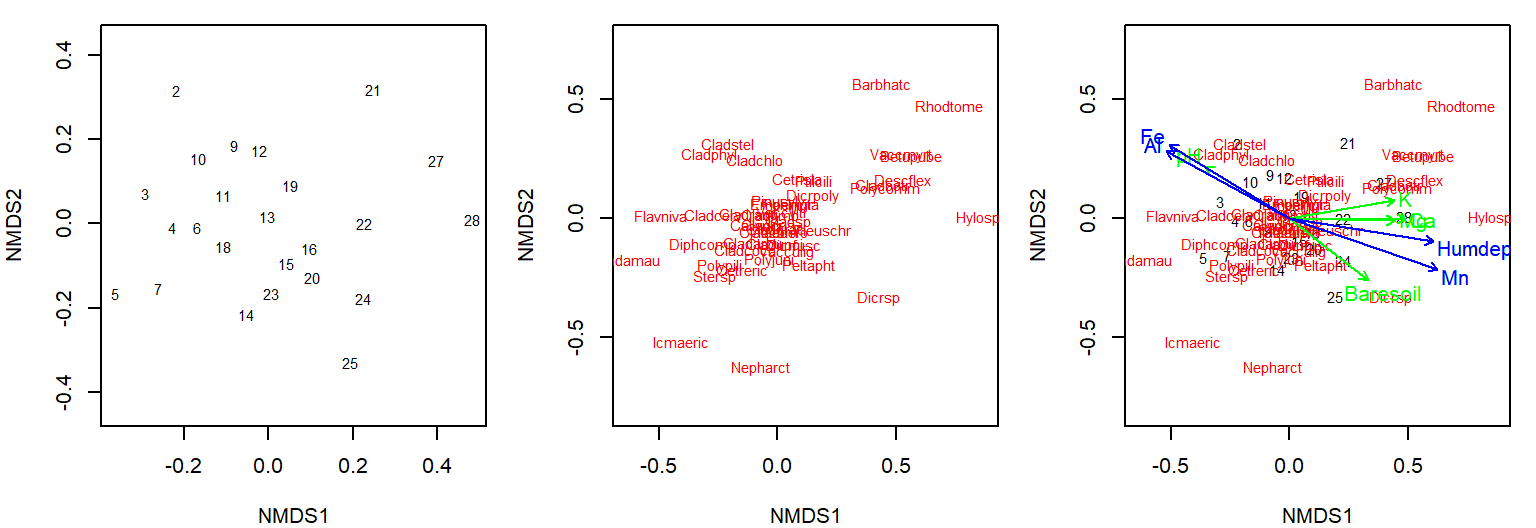
\includegraphics[width=1\linewidth,height=1\textheight]{_main_files/figure-latex/vare-ord-1} 

}

\caption{vare- data from vegan showing sites only, species only, and both plus environmental overlays.}\label{fig:vare-ord}
\end{figure}

See how the multivariate analysis has taken all those data, both species and environmental, and `communicated' them in one single figure? You can see numerous relationships (both positive and negative) in this figure, and species-site-environment associations. It also illustrates a potential challenge with multivariate ordinations. It is very easy to get cluttered and overloaded. There is no easy way around this, though there is further help in these packages.

You are in charge of the analysis. You can change the emphasis and elements of the message depending on your data transformation, dissimilarity metric, and ordination technique (hence `black art'). There is no absolutely `correct' way to go about multivariate stats, so different statisticians will have their favoured approaches and methods.

Note: Some functions (e.g.~\texttt{metaMDS()}) default to autotransform your data if the function thinks it is necessary. This can be useful but, in scientific reports, you must specify what transformations you used. Here you don't know what the function applies as it depends on the data, but it could be the square or fourth-root and/or Wisconsin transformation (which is a double standardisation). My advice is only to use transformations that you specify.

\begin{center}\rule{0.5\linewidth}{0.5pt}\end{center}

\hypertarget{principal-components-analysis-pca}{%
\section{Principal components analysis (PCA)}\label{principal-components-analysis-pca}}

PCA is a long-established multivariate technique that is often applied to `environmental' data rather than `count' data. Environmental data is, usually, quite different from species count data in that most environmental parameters (e.g.~metal concentrations) are present, at least to some degree. This contrasts to species data where many species are often absent (zeros). These zero counts would lead to problems if analysed using PCA, since PCA would `think' that sites that shared lots of `absences' were more similar, which is not necessarily desirable.

With environmental data, such as temperature, light, and concentration, zeros tend to be less prevalent. However, environmental data (e.g.~that describing your sampling location in space and time) might include all manner of different variables on different scales (e.g., radient flux in lumens, temperature in C, nutrient/contaminant concentrations in mg/l). What you wouldn't wish to see is your arbitrary choice of measurement unit (e.g., C or K) having any influence on your analysis such that a variable is given more weight simply because the numbers are larger.

Instead, we want all of our variables to be treated `equally'. You can do all this by setting \texttt{pcomp(...,\ scale=TRUE)}. Scaling means that each measurement is expressed in units of standard deviation (a Z-score!!). Usually it is desirable to center the data as well by subtracting the mean. Centering and scaling means that each of the environmental variables is of `equal importance' regardless of the magnitude of the raw values.

A basic, and very friendly, introduction to PCA is given in Chapter 4 of \href{https://www.primer-e.com/wp-content/uploads/2018/10/Change-in-Marine-Communities-3rd-ed.pdf}{Clarke et al.~2014}.

The data set we'll look at here is from SAMS Professor Tom Wilding's PhD thesis. He set up an experiment to examine the relative leach\_dfing of trace metals from concrete, granite, and a control (artificial seawater). Concrete contains cement which is enriched in vanadium and molybdenum, and these elements could leach\_df out in dangerous amounts. Granite, the main constituent of this concrete, might also leach\_df some trace elements. He suspended concrete and granite powder in artificial water, constantly agitated it, and measured the leach\_dfate concentrations over 100 days \href{https://doi.org/10.1006/jmsc.2002.1267}{Wilding and Sayer 2002}.

\begin{Shaded}
\begin{Highlighting}[]
\FunctionTok{library}\NormalTok{(readxl)}
\FunctionTok{library}\NormalTok{(tidyverse)}
\NormalTok{leach\_df }\OtherTok{\textless{}{-}} \FunctionTok{read\_excel}\NormalTok{(}\StringTok{"data/practical\_5.xlsx"}\NormalTok{, }\AttributeTok{sheet =} \StringTok{"Leaching"}\NormalTok{) }\SpecialCharTok{|\textgreater{}}
  \FunctionTok{mutate}\NormalTok{(}\AttributeTok{Treat\_abbr =} \FunctionTok{factor}\NormalTok{(Treat, }\CommentTok{\# abbreviate for cleaner plotting}
                             \AttributeTok{levels =} \FunctionTok{c}\NormalTok{(}\StringTok{"concrete"}\NormalTok{, }\StringTok{"control"}\NormalTok{, }\StringTok{"granite"}\NormalTok{),}
                             \AttributeTok{labels =} \FunctionTok{c}\NormalTok{(}\StringTok{"conc"}\NormalTok{, }\StringTok{"ctrl"}\NormalTok{, }\StringTok{"gran"}\NormalTok{)),}
         \AttributeTok{Treat\_day =} \FunctionTok{paste}\NormalTok{(Treat\_abbr, Day, }\AttributeTok{sep=}\StringTok{"\_"}\NormalTok{), }\CommentTok{\# treat + days in exprmnt}
         \AttributeTok{Conc =} \FunctionTok{signif}\NormalTok{(Conc)) }\SpecialCharTok{|\textgreater{}}
  \FunctionTok{select}\NormalTok{(Treat\_day, Element, Conc) }\CommentTok{\# remove columns that aren\textquotesingle{}t of use,}
\CommentTok{\#summary(leach\_df)}

\CommentTok{\# not dominated by zeros; try other values (e.g. \textless{}10)}
\FunctionTok{table}\NormalTok{(leach\_df}\SpecialCharTok{$}\NormalTok{Conc }\SpecialCharTok{==} \DecValTok{0}\NormalTok{) }
\end{Highlighting}
\end{Shaded}

\begin{verbatim}
## 
## FALSE  TRUE 
##   143     4
\end{verbatim}

\begin{Shaded}
\begin{Highlighting}[]
\FunctionTok{mean}\NormalTok{(leach\_df}\SpecialCharTok{$}\NormalTok{Conc }\SpecialCharTok{==} \DecValTok{0}\NormalTok{) }\CommentTok{\# recall that R treats T/F as 1/0 }
\end{Highlighting}
\end{Shaded}

\begin{verbatim}
## [1] 0.02721088
\end{verbatim}

\begin{Shaded}
\begin{Highlighting}[]
\FunctionTok{par}\NormalTok{(}\AttributeTok{mfrow=}\FunctionTok{c}\NormalTok{(}\DecValTok{1}\NormalTok{,}\DecValTok{1}\NormalTok{))}
\FunctionTok{hist}\NormalTok{(leach\_df}\SpecialCharTok{$}\NormalTok{Conc, }\AttributeTok{main =} \ConstantTok{NULL}\NormalTok{) }
\end{Highlighting}
\end{Shaded}

\begin{figure}

{\centering 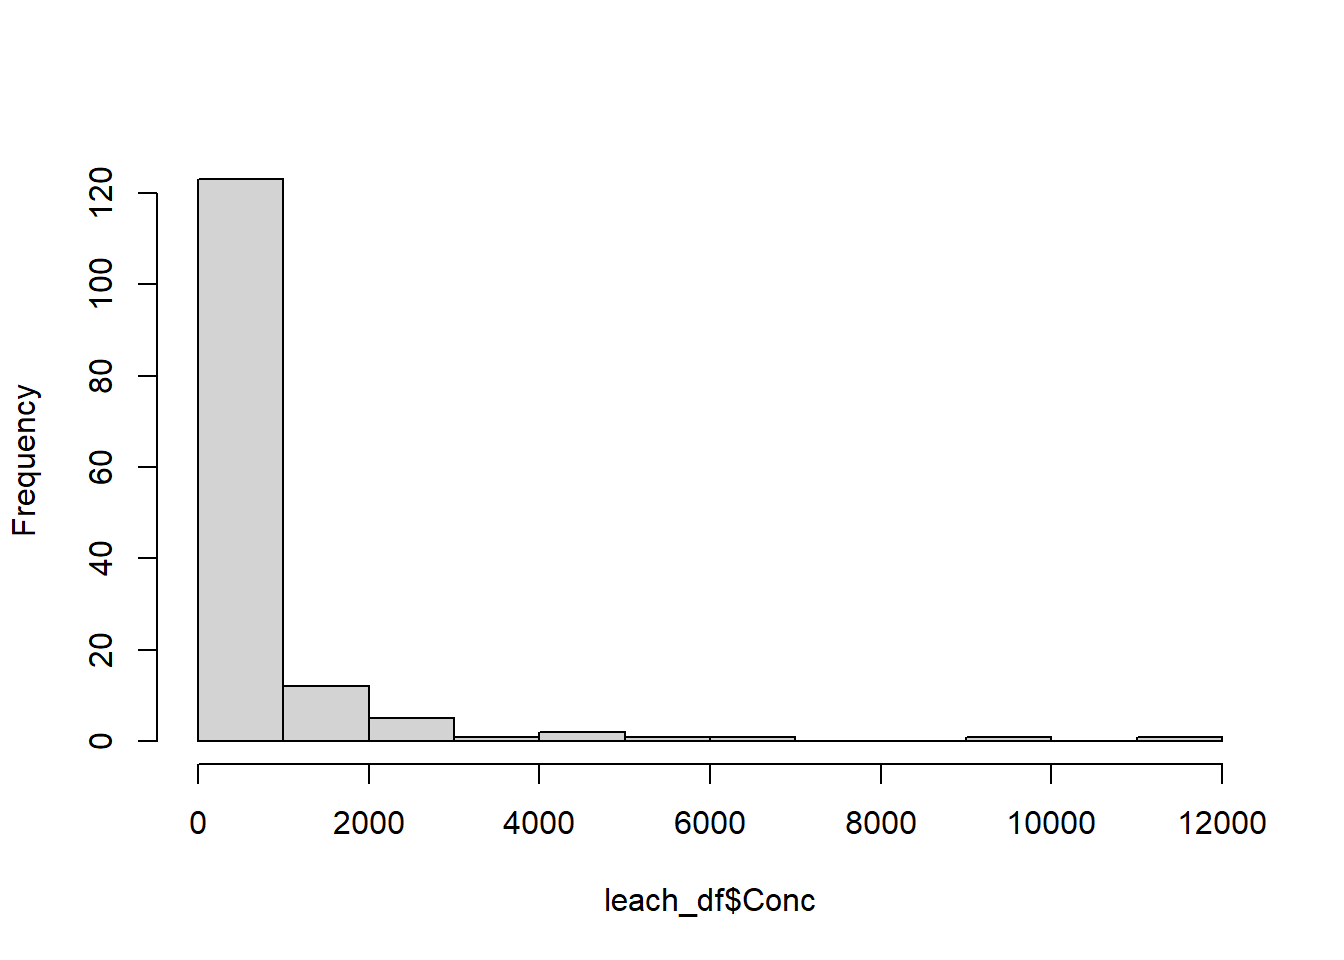
\includegraphics[width=0.5\linewidth,height=0.5\textheight]{_main_files/figure-latex/leach-hist-1} 

}

\caption{Histogram of leaching data (raw) illustrating the wide range of values and skew.}\label{fig:leach-hist}
\end{figure}

Next, we need to re-organise the data into a wider format so that each element is a column and each row is a sample.

\begin{Shaded}
\begin{Highlighting}[]
\NormalTok{leach\_df\_wide }\OtherTok{\textless{}{-}}\NormalTok{ leach\_df }\SpecialCharTok{|\textgreater{}}
  \FunctionTok{pivot\_wider}\NormalTok{(}\AttributeTok{names\_from=}\StringTok{"Element"}\NormalTok{, }\AttributeTok{values\_from=}\StringTok{"Conc"}\NormalTok{)}
\end{Highlighting}
\end{Shaded}

The column \texttt{Treat\_day} is coded as \texttt{trt\_day}, where \texttt{trt} is the 4 letter code indicating treatment type and \texttt{day} is the number of days elapsed in the experiment (one of 1, 4, 7, 17, 32, 50 or 100). So \texttt{gran\_32} means the granite treatment sampled at day 32.

We can calculate the principal components using \texttt{prcomp()}, subsetting the dataframe to give only the columns with element concentrations (i.e., removing \texttt{Treat\_day}, which is the first column). We'll also set the arguments for centering and scaling to \texttt{TRUE}.

\begin{Shaded}
\begin{Highlighting}[]
\NormalTok{PCA\_leach }\OtherTok{\textless{}{-}} \FunctionTok{prcomp}\NormalTok{(leach\_df\_wide[, }\SpecialCharTok{{-}}\DecValTok{1}\NormalTok{], }\AttributeTok{center =} \ConstantTok{TRUE}\NormalTok{, }\AttributeTok{scale =} \ConstantTok{TRUE}\NormalTok{) }
\FunctionTok{screeplot}\NormalTok{(PCA\_leach, }\AttributeTok{main =} \ConstantTok{NULL}\NormalTok{, }\AttributeTok{ylab =} \StringTok{"Relative variation explained"}\NormalTok{)}
\end{Highlighting}
\end{Shaded}

\begin{figure}

{\centering \includegraphics[width=0.5\linewidth,height=0.5\textheight]{_main_files/figure-latex/leach-scree-1} 

}

\caption{Scree plot showing the variance explained by each principal component.}\label{fig:leach-scree}
\end{figure}

\begin{Shaded}
\begin{Highlighting}[]
\CommentTok{\# take a look at PCA\_leach}
\NormalTok{PCA\_leach}
\FunctionTok{str}\NormalTok{(PCA\_leach)}
\end{Highlighting}
\end{Shaded}

You can see from the screeplot that the amount variance explained declines with principal component as expected and that there is very little variation left afer 3 principal components. That is, nearly all of the variation in the dataset is captured by PC1, PC2, and PC3. In this case, PCA has essentially solved the `curse of dimensionality' by successfully reducing 7 dimensional data to about three.

Data transformations are critical to PCA analysis, as they are with NMDS. In most PCAs you center and standardize your data so that each column is on the same scale.

We can plot our results using \texttt{biplot()} which has some helpful defaults including labels for the samples (\texttt{Treat\_day}) and the correlation strength of each element with PC1 and PC2:

\begin{Shaded}
\begin{Highlighting}[]
\FunctionTok{biplot}\NormalTok{(PCA\_leach, }\AttributeTok{xlabs =}\NormalTok{ leach\_df\_wide}\SpecialCharTok{$}\NormalTok{Treat\_day, }\AttributeTok{cex =} \FloatTok{0.75}\NormalTok{)}
\end{Highlighting}
\end{Shaded}

\begin{figure}

{\centering \includegraphics[width=0.5\linewidth,height=0.5\textheight]{_main_files/figure-latex/leach-biplot1-1} 

}

\caption{PCA of the complete dataset, illustrating the common challenge of overplotting.}\label{fig:leach-biplot1}
\end{figure}

To plot more than 2 dimensions you could use a 3D plot, but these are frankly difficult to interpret since it is reduced \emph{back} to 2D on a page or computer screen. Another option is to use colour for the 3\textsuperscript{rd} axis. Here's an example using \texttt{ggplot2}. Adding arrows showing the loadings (see below) is possible, but more work.

\begin{Shaded}
\begin{Highlighting}[]
\NormalTok{PCA\_leach}\SpecialCharTok{$}\NormalTok{x }\SpecialCharTok{|\textgreater{}}
  \FunctionTok{as\_tibble}\NormalTok{() }\SpecialCharTok{|\textgreater{}}
  \FunctionTok{mutate}\NormalTok{(}\AttributeTok{Treat\_day =}\NormalTok{ leach\_df\_wide}\SpecialCharTok{$}\NormalTok{Treat\_day) }\SpecialCharTok{|\textgreater{}}
  \FunctionTok{ggplot}\NormalTok{(}\FunctionTok{aes}\NormalTok{(PC1, PC2, }\AttributeTok{colour =}\NormalTok{ PC3, }\AttributeTok{label =}\NormalTok{ Treat\_day)) }\SpecialCharTok{+} 
  \FunctionTok{geom\_label}\NormalTok{(}\AttributeTok{size =} \DecValTok{3}\NormalTok{, }\AttributeTok{fill =} \ConstantTok{NA}\NormalTok{) }\SpecialCharTok{+}
  \FunctionTok{scale\_colour\_gradient2}\NormalTok{(}\AttributeTok{mid =} \StringTok{"cornsilk2"}\NormalTok{) }\SpecialCharTok{+}
  \FunctionTok{theme\_bw}\NormalTok{()}
\end{Highlighting}
\end{Shaded}

\begin{figure}

{\centering \includegraphics[width=0.5\linewidth,height=0.5\textheight]{_main_files/figure-latex/leach-biplot1-gg-1} 

}

\caption{PCA of the complete dataset using ggplot2.}\label{fig:leach-biplot1-gg}
\end{figure}

The ordination plots the relative positions (in terms of similiarity) of the samples. There are numerous label overlaps making the interpretation of the ordination difficult. If you were producing this for publication you would need to sort this out.

\emph{Q156. Which elements are positivley associated with granite and concrete, particulalry after longer periods of leaching?}

As is typical, overlapping points make interpretation more difficult. There are elegant solutions to this (in terms of labelling) but for now, we'll split the data and analyse it separately.

We'll need more data wrangling to split it efficiently and we'll use \texttt{grepl()}, which identifies a pattern within a character using a regular expression (a.k.a., regex), returning a \texttt{TRUE} or \texttt{FALSE} for each element in the character vector. Here, we'll filter the dataframe to only include rows where \texttt{Treat\_day} contains \texttt{conc} or \texttt{gran}. Remember the `or' operator \texttt{\textbar{}}?

\begin{Shaded}
\begin{Highlighting}[]
\CommentTok{\#?grepl}
\CommentTok{\#cbind(leach\_df\_wide$Treat\_day, grepl("conc|gran", leach\_df\_wide$Treat\_day))}
\NormalTok{leach\_df\_trts }\OtherTok{\textless{}{-}}\NormalTok{ leach\_df\_wide }\SpecialCharTok{|\textgreater{}}
  \FunctionTok{filter}\NormalTok{(}\FunctionTok{grepl}\NormalTok{(}\StringTok{"conc|gran"}\NormalTok{, Treat\_day))}
\NormalTok{PCA\_trts }\OtherTok{\textless{}{-}} \FunctionTok{prcomp}\NormalTok{(leach\_df\_trts[, }\SpecialCharTok{{-}}\DecValTok{1}\NormalTok{], }\AttributeTok{scale =} \ConstantTok{TRUE}\NormalTok{, }\AttributeTok{center =} \ConstantTok{TRUE}\NormalTok{)}
\FunctionTok{biplot}\NormalTok{(PCA\_trts, }\AttributeTok{xlabs =}\NormalTok{ leach\_df\_trts}\SpecialCharTok{$}\NormalTok{Treat\_day)}
\end{Highlighting}
\end{Shaded}

\begin{figure}

{\centering \includegraphics[width=0.5\linewidth,height=0.5\textheight]{_main_files/figure-latex/leach-biplot2-1} 

}

\caption{PCA of the concrete and granite, illustrating temporal and treatment differences.}\label{fig:leach-biplot2}
\end{figure}

\emph{Q157. Repeat the analysis, but set \texttt{scale\ =\ FALSE}. Which element now seems to dominate the analysis? Explain what you see.}

A PCA is normally reported with the proportion of the variation explained by each of the principal components (and the cumulative proportion). If the cumulative proportion for the 1st two PCs is high, then your 2D (PC1 and PC2) ordination is a good representation of the similarities between samples. In that sense a high cumulative proportion is analogous to a low stress (for NMDS).

Let's have a look at a summary of the principal components.

\begin{Shaded}
\begin{Highlighting}[]
\NormalTok{PCA\_leach\_summary }\OtherTok{\textless{}{-}} \FunctionTok{summary}\NormalTok{(PCA\_leach) }
\CommentTok{\#PCA\_leach\_summary}
\CommentTok{\#str(PCA\_leach\_summary)}
\NormalTok{PCA\_leach\_summary}\SpecialCharTok{$}\NormalTok{importance[, }\DecValTok{1}\SpecialCharTok{:}\DecValTok{4}\NormalTok{] }\CommentTok{\# extract only PC1{-}4}
\end{Highlighting}
\end{Shaded}

\begin{verbatim}
##                             PC1      PC2       PC3       PC4
## Standard deviation     1.988091 1.450775 0.7782675 0.5599535
## Proportion of Variance 0.564640 0.300680 0.0865300 0.0447900
## Cumulative Proportion  0.564640 0.865320 0.9518500 0.9966400
\end{verbatim}

As you can see, PC1, PC2, and PC3 capture more than 95\% of the variance in our data. Adding PC4 brings that up above 99\%.

Finally, we can look at factor loadings. This is a measure of how each feature (metal concentration in this case) relates to the principal components. In PCA, the principal components are sequentially `less' influential since they describe increasingly smaller amounts of variation. By centering and standardising your response variables, you can assess the relative importance of each in driving the patterns you observe in your ordination. The magnitude is what we're interested in rather than the sign.

In an object created by \texttt{prcomp()}, the loadings are stored as \texttt{.\$rotation}.

\begin{Shaded}
\begin{Highlighting}[]
\CommentTok{\# ?prcomp}
\CommentTok{\# str(PCA\_leach)}
\FunctionTok{signif}\NormalTok{(PCA\_leach}\SpecialCharTok{$}\NormalTok{rotation[, }\DecValTok{1}\SpecialCharTok{:}\DecValTok{5}\NormalTok{], }\DecValTok{3}\NormalTok{) }\CommentTok{\# factor loadings for PC1{-}5}
\end{Highlighting}
\end{Shaded}

\begin{verbatim}
##       PC1     PC2     PC3    PC4      PC5
## Ba -0.367  0.2090  0.6510 -0.619 -0.00405
## Fe -0.380 -0.0440 -0.7370 -0.553  0.01420
## Mn -0.146  0.6500 -0.0963  0.211  0.67300
## Mo -0.430 -0.3360  0.0795  0.283 -0.09810
## Rb -0.462 -0.2440  0.0327  0.305  0.21600
## Sr -0.495 -0.0788  0.0663  0.168  0.01510
## U  -0.238  0.5940 -0.1110  0.254 -0.70000
\end{verbatim}

Here you can see that Sr, Rb, Mo are relatively `important' in driving the multivariate pattern you've observed (i.e., high absoluate values on PC1) while Mn and U have high values for PC2 (you could say that PC2 accounts for Mn and U).

\begin{center}\rule{0.5\linewidth}{0.5pt}\end{center}

\hypertarget{conclusions-5}{%
\section{Conclusions}\label{conclusions-5}}

I will let you write your own summary and conclusions from this practical as this will help you consolidate your understanding. You may wish to consider the following: the nature of multivariate vs.~univariate data, types and characteristics of multivariate data (e.g.~counts vs.~environmental data), the analytical methods introduced here for dealing with data of different types, the purpose and effect of transformations and standardisations and where they are used, the use of summary metrics (e.g.~diversity metrics) and their advantages and disadvantages. You should also be familiar with the interpretation of simple ordinations (both PCA and NMDS) and the concept of stress and `proportion explained' (for NMDS and PCA respectively).

\hypertarget{appendix}{%
\chapter{Appendix}\label{appendix}}

\hypertarget{probability}{%
\section{Probability}\label{probability}}

\hypertarget{probability-for-equally-likely-outcomes}{%
\subsection{Probability for equally likely outcomes}\label{probability-for-equally-likely-outcomes}}

The probability of event \(A\) occuring is \(P(A) = \frac{r}{n}\), where \(n\) is the number of trials and \(r\) is the number of trials during which \(A\) occurred.

\hypertarget{multiplication-and-addition}{%
\subsection{Multiplication and addition}\label{multiplication-and-addition}}

The general case of the multiplication rule is that, for two events \(A\) and \(B\):

\(P(A \& B) = P(A) * P(B|A)\), where \(P(B|A)\) is the probability that \(B\) occurs given than \(A\) has already occurred.

The Addition Law states that, for two events \(A\) and \(B\):

\(P(A\ or\ B\ or\ A\&B) = P(A) + P(B) - P(A\&B)\)

and

\(P(A\ or\ B\ but\ not\ A\&B) = P(A) + P(B) - 2*P(A\&B)\)

and when \(A\) and \(B\) are mutually exclusive, then:

\(P(A\ or\ B) = P(A) + P(B)\)

\hypertarget{bayes-theorem}{%
\subsection{Bayes' theorem}\label{bayes-theorem}}

\(P(A|B)= \frac{P(B|A) * P(A)}{P(B)}\), where \(P(B)= P(A) * P(B|A) + P(A’) * P(B|A’)\).

\hypertarget{univariate-statistics}{%
\section{Univariate statistics}\label{univariate-statistics}}

\hypertarget{mean}{%
\subsection{Mean}\label{mean}}

\texttt{mean()}

The mean is calculated as \(\bar{y} = \frac{\sum{y}}{n}\).

For measures of central tendency and dispersion, we use greek letters to refer to population values and latin letters to refer to samples:

\begin{longtable}[]{@{}lll@{}}
\toprule()
& Population & Sample \\
\midrule()
\endhead
Mean & \(\mu\) & \(\bar{y}\) \\
Variance & \(\sigma^2\) & \(s^2\) \\
Standard deviation & \(\sigma\) & \(s\) \\
\bottomrule()
\end{longtable}

\hypertarget{median-quartiles-and-adjacent-values}{%
\subsection{Median, quartiles and adjacent values}\label{median-quartiles-and-adjacent-values}}

\texttt{median()}, \texttt{quantile()}, \texttt{IQR()}

With data ordered by rank, the median value is the middle value or the \((\frac{n+1}{2})^{th}\) value, the lower quartile, \(Q1\), is the \((\frac{n+1}{4})^{th}\) value, the upper quartile, \(Q3\), is the \((\frac{3*(n+1)}{2})^{th}\) value. The inter-quartile range is \(IQR = Q3 – Q1\). The upper adjacent value is the upper value that is less than \(Q3 + (1.5 * IQR)\). The lower adjacent value is the lower value that is more than the \(Q1 – (1.5 * IQR)\). Outliers are defined as values that lie outside the range \(Q1 - 1.5*IQR\) or \(Q3 + 1.5*IQR\).

\hypertarget{the-sum-of-squares}{%
\subsection{The sum of squares}\label{the-sum-of-squares}}

The sum of squares is given by \(SS = \sum{y^2} - \frac{(\sum{y})^2}{n}\) where \(n\) is the number of observations.

\hypertarget{measures-of-dispersion}{%
\subsection{Measures of dispersion}\label{measures-of-dispersion}}

\texttt{var()}, \texttt{sd()}, \texttt{length()}

When dealing with \textbf{populations} the following formulae are used:

\textbf{Variance:} \(\sigma^2 = \frac{SS}{n}\)

\textbf{Standard deviation:} \(\sigma = \sqrt{\frac{SS}{n}} = \sqrt{\sigma^2}\)

When dealing with \textbf{samples} the following formulae are used:

\textbf{Variance:} \(s^2 = \frac{SS}{n-1}\)

\textbf{Standard deviation:} \(s = \sqrt{\frac{SS}{n-1}}\)

\hypertarget{the-binomial-distribution-2}{%
\section{The Binomial distribution}\label{the-binomial-distribution-2}}

\texttt{dbinom()}, \texttt{pbinom()}, \texttt{qbinom()}, \texttt{rbinom()}

The binomial distribution describes the expected distribution for two mutually exclusive outcomes. The formula is given by:\\
\(P(x) = \frac{n!}{x!(n-x)!} p^x q^{n-x}\)

where \(P(x)\) is the probability of \(x\) `successes' occurring, \(n\) is the number of trials, \(p\) is the probability of \(x\) in a single trial, and \(q\) is the probability of \emph{not} \(x\) in a single trial with \(p+q=1\).

A binomially distributed variable has \textbf{mean} = \(n*p\) and \textbf{variance} = \(n*p*q\).

\hypertarget{the-poisson-distribution-1}{%
\section{The Poisson distribution}\label{the-poisson-distribution-1}}

\texttt{dpois()}, \texttt{ppois()}, \texttt{qpois()}, \texttt{rpois()}

The Poisson distribution for a sample is defined as follows:

\(P(x) = \frac{\bar{x}^x e^{-x}}{x!}\)

where \(\bar{x}\) is the sample mean and \(x\) is the value (count) of interest.

\hypertarget{z-scores}{%
\section{Z scores}\label{z-scores}}

\texttt{scale()}

The \emph{standard normal distribution} is \(Norm(\mu=0, \sigma=1)\). Z scores are used to convert any normal distribution to the standard normal distribution:

\(z = \frac{y-\mu}{\sigma}\)

where \(y\) is the value, \(\mu\) is the mean of the population and \(\sigma\) is the standard deviation of the population.

\hypertarget{samples-taken-from-a-population}{%
\section{Samples taken from a population}\label{samples-taken-from-a-population}}

\texttt{sd()}, \texttt{sqrt()}, \texttt{length()}, \texttt{mean()}, \texttt{sqrt()}

\hypertarget{standard-error-of-the-mean}{%
\subsection{Standard error of the mean}\label{standard-error-of-the-mean}}

The \emph{standard error} is the standard deviation of sample means:

\(SEM = \sigma_{\bar{y}} = \frac{\sigma}{\sqrt{n}}\)

where \(\sigma\) is the population standard deviation and \(n\) is the sample size. If we are testing a sample taken from a population \emph{of known population mean and population standard deviation} we use the formula:

\(z = \frac{\bar{y}-\mu}{\sigma_{\bar{y}}}\)

where \(\bar{y}\) is a particular sample mean, \(\mu\) is the population mean, and \(\sigma_{\bar{y}}\) is the standard error of the mean.

\hypertarget{the-t-distribution}{%
\section{The t distribution}\label{the-t-distribution}}

\texttt{dt()}, \texttt{pt()}, \texttt{qt()}, \texttt{rt()}

The t-distribution describes the distribution of \(T\) statistics expected under the null hypothesis.

\hypertarget{the-one-sample-t-test}{%
\subsection{The one sample t-test}\label{the-one-sample-t-test}}

\texttt{t.test()}

The T statistic is calculated as:

\(T = \frac{\bar{y}-\mu}{s_{\bar{y}}}\)

Where \(\bar{y}\) is the sample mean, \(\mu\) is the hypothesized population mean, and \(s_{\bar{y}}\) is the standard error such that \(s_{\bar{y}} = \frac{s}{\sqrt{n}}\) with sample standard deviation \(s\).

Use \texttt{t.test()}, or find the p-value associated with your T with \texttt{pt(T,\ df-1)}.

\hypertarget{confidence-intervals-for-sample-means}{%
\subsection{Confidence intervals for sample means}\label{confidence-intervals-for-sample-means}}

\texttt{t.test()}, \texttt{qt()}, \texttt{mean()}, \texttt{sd()}, \texttt{length()}, \texttt{sqrt()}

The 95\% CI for a mean is calculated as:

\(\bar{y} \pm t_{\alpha/2, df=n-1} * s_{\bar{y}}\)

\hypertarget{anova}{%
\section{ANOVA}\label{anova}}

\texttt{anova(lm())}, \texttt{aov()}

An ANOVA table contains the following:

\begin{longtable}[]{@{}
  >{\raggedright\arraybackslash}p{(\columnwidth - 8\tabcolsep) * \real{0.2877}}
  >{\raggedright\arraybackslash}p{(\columnwidth - 8\tabcolsep) * \real{0.2192}}
  >{\raggedright\arraybackslash}p{(\columnwidth - 8\tabcolsep) * \real{0.2740}}
  >{\raggedright\arraybackslash}p{(\columnwidth - 8\tabcolsep) * \real{0.1781}}
  >{\raggedright\arraybackslash}p{(\columnwidth - 8\tabcolsep) * \real{0.0411}}@{}}
\toprule()
\begin{minipage}[b]{\linewidth}\raggedright
Source of variation
\end{minipage} & \begin{minipage}[b]{\linewidth}\raggedright
Sum of Squares
\end{minipage} & \begin{minipage}[b]{\linewidth}\raggedright
Degrees of Freedom
\end{minipage} & \begin{minipage}[b]{\linewidth}\raggedright
Mean Square
\end{minipage} & \begin{minipage}[b]{\linewidth}\raggedright
F
\end{minipage} \\
\midrule()
\endhead
Between groups & \({SS}_{groups}\) & \({df}_{groups}\) & \(\frac{{SS}_{groups}}{{df}_{groups}}\) & \(\frac{{MS}_{groups}}{{MS}_{error}}\) \\
Error & \({SS}_{error}\) & \({df}_{error}\) & \(\frac{{SS}_{error}}{{df}_{error}}\) & \\
Total & \({SS}_{total}\) & \({df}_{total}\) & & \\
\bottomrule()
\end{longtable}

with:

\({SS}_{groups} = \sum{n_j (\bar{y_j} - \bar{\bar{y}})^2}\)

\({SS}_{error} = \sum{(y_{ij} - \bar{y_j})^2}\)

\({SS}_{total} = {SS}_{groups} + {SS}_{error} = \sum{(y_{ij} - \bar{\bar{y}})^2}\)

where \(y_{ij}\) is the \(i^{th}\) observation in group \(j\), \(\bar{y_j}\) is the mean for group \(j\), and \(\bar{\bar{y}}\) is the grand mean. With \(N\) total observations, \(n_j\) observations per group, and \(k\) groups, the degrees of freedom are:

\({df}_{groups} = k - 1\)

\({df}_{error} = N - k = k (n_j-1)\)

\({df}_{total} = {df}_{groups} + {df}_{error} = N-1\)

The critical value (CV) for samples of equal size is given as:

\(CV = q \sqrt{\frac{{MS}_{error}}{n}}\)

where \(q\) either comes from a table online (the \emph{studentized range distribution}), or from \texttt{qtukey(1-alpha,\ k,\ df\_error)}.

\hypertarget{regression-correlation}{%
\section{Regression \& correlation}\label{regression-correlation}}

\texttt{lm()}, \texttt{cor()}, \texttt{confint()}, \texttt{predict()}

We do not bother calculating regression coefficients by hand.

\end{document}
